\documentclass[12pt]{report}
\usepackage[utf8]{inputenc}
\usepackage{amsmath}
\usepackage{xcolor, soul}
\sethlcolor{yellow}
\usepackage{amsfonts}
\usepackage{venndiagram}
\usepackage{geometry}
\usepackage{hyperref}
\geometry{margin=1.1in}

\title{Sistemi Operativi}
\author{Cosimo Botticelli}
\date{2021}

\begin{document}
\maketitle
\tableofcontents


\chapter{Parte Prima, Capitolo 1: Introduzione}
    \vspace{3mm}
    \section{Filosofia di questi appunti e perché dovrebbe fregartene qualcosa}
        \textbf{tl;dr} Il codice \LaTeX di questi appunti è pubblico e modificabile all'hyperlink gigante in basso.
        
        \textbf{Versione lunga}: inizialmente ho creato questi appunti solo per me, poi li ho condivisi, poi ho aggiunto un link di donazioni.
        
        Vedendo un po' di gente usarli e farli girare, ho pensato di poter creare qualcosa di più interessante di un pacco di appunti che fra qualche anno sarà datato e un guadagno di qualche spicciolo per me: vorrei creare un punto di raccolta per tutti gli studenti Unisa e non, per trovare, inserire e aggiornare appunti. In questo modo spero che lo sforzo di gruppo fornisca una fonte gratuita, libera, collettiva e soprattutto aggiornata di conoscenza, anche quando i corsi inevitabilmente verranno aggiornati e quando io, fra circa 12 ere geologiche, mi laureerò.
        
        \vspace{3mm}
        
        Oltre alla partecipazione ai singoli documenti, mi farebbe piacere aggiungere collaboratori per dividerci la gestione della repository, e che possano magari ereditarla del tutto quando perché non ho intenzione di accettare pull request per tutta la vita.
    \begin{figure}[h]
        \centering
        \href{https://github.com/shyimon/UnisaComeBabele}
        {
\includegraphics[width=0.9\textwidth]{Images/github.png}}
    \end{figure}
\section{Introduzione}
    \begin{center}
        \Large\color{red}!!!DISCLAIMER!!!
    \end{center}
    Questo corso si basa fortemente sullo studio del libro \textit{Sistemi Operativi: Concetti ed Esempi} di \textit{Abraham Silberschatz}. I seguenti appunti fungono dunque da guida e riassunto di quanto studiato sul libro, ma non hanno una funzione sostitutiva. I riferimenti a pagine e capitoli del libro sono riguardanti la decima edizione Italiana.
    
    L'obiettivo di questo corso, dal punto di vista teorico, è capire con un certo livello di precisione e dettaglio cosa sia un sistema operativo, le motivazioni dietro lo stesso e come funzioni. Dal punto di vista pratico sarà scrivere un programma che invoca correttamente delle \texttt{syscall} (system calls). Questo percorso ha inizio con questa prima parte, che comprende delle definizioni di base di sistema operativo, dei cenni storici e uno studio della struttura di un sistema operativo.
    
\section{Cosa è un Sistema Operativo}
    Un Sistema Operativo è innanzitutto un \textbf{programma}, nonostante abbia struttura e funzioni piuttosto diverse da quelle dei programmi con cui siamo abituati a interagire.
    
    Per capire la funzione di un SO e in che modo è diverso da tutti gli altri programmi, ci conviene posizionarlo all'interno di un contesto software e hardware:
    
    \begin{figure}[h]
        \centering
        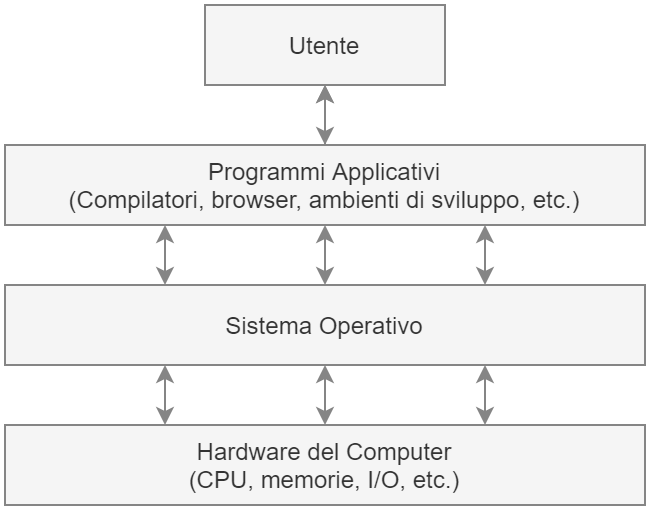
\includegraphics[width=0.6\textwidth]{img/img1.png}
        \caption{Componenti di un sistema elaborativo.}
        \label{fig:img1}
    \end{figure}
    
    Facciamo dunque una suddivisione dell'intero sistema elaborativo in quattro componenti, e in particolare vediamo che l'\textbf{hardware} fornisce al sistema le risorse di memorizzazione ed elaborative fondamentali, mentre i \textbf{programmi applicativi} definiscono il modo in cui queste risorse vengono usate nella risoluzione di problemi computazionali degli \textbf{utenti}, i quali si interfacciano con i suddetti programmi. 
    
    In tutto ciò, il ruolo del \textbf{sistema operativo} è quello di offrire gli strumenti per impiegare in modo corretto le risorse offerte. Il suo ruolo, per fare un'analogia politica, è simile a quello di un \textit{governo}, che non svolge funzioni effettivamente utili, ma fornisce un ambiente nel quale altri enti/programmi possono lavorare in modo utile.
    
    Per meglio capire il ruolo del sistema operativo, e per avere un altro punto di vista, lo esploriamo da due punti di vista: quello dell'utente e quello del sistema.
    
    \subsection{Punto di vista dell'utente}
        Dal punto di vista di un utente che usa un determinato dispositivo, la cosa più importante è la \textbf{facilità d'uso}. I sistemi operativi odierni sono generalmente progettati per l'utilizzo da parte di un singolo utente, con grande attenzione alla suddetta facilità d'uso, qualche accortezza riguardante le prestazioni, ma nessuna all'\textbf{utilizzo delle risorse}, a come cioè sono condivise le risorse hardware e software.
        
        Un altro punto da prendere in considerazione è la varietà dei dispositivi utilizzati dai vari utenti, che possono andare dai più classici personal computer dotati di schermo, tastiera e mouse, agli smartphone, dotati di touch screen e assistenti vocali, a dispositivi \textbf{embedded} presenti in elettrodomestici e simili, che possono interfacciarsi con l'utente in maniera molto minimale, tramite magari una tastiera numerica, qualche tasto e dei led per indicarne lo stato.
        
    \subsection{Punto di vista del sistema}
        Dal punto di vista del calcolatore, il sistema operativo è il programma più strettamente correlato al suo hardware. In tale contesto è possibile considerare un sistema operativo come un \textbf{assegnatore di risorse}.
        
        Un altro modo per vedere il sistema operativo è come programma di controllo che gestisce l'esecuzione di programmi utenti in modo da impedire eventuali errori o che il calcolatore sia usato in modo scorretto, e che si occupa del controllo dei dispositivi I/O, con un'enfasi non primaria sull'ottimizzazione delle risorse.
        
    \subsection{Definizione di Sistema Operativo}
        A questo punto abbiamo capito che non è semplicissimo dare una definizione precisa di sistema operativo. Esso definisce diversi ruoli e funzionalità e ciò può variare in base alla natura del sistema hardware, ai target users e tanti altri parametri.
        
        Nonostante tutto ciò, per i nostri scopi il sistema operativo include il kernel (nucleo) sempre in esecuzione, i framework middleware che facilitano lo sviluppo di applicazioni e forniscono altre funzionalità e i programmi di sistema che contribuiscono alla gestione dello stesso mentre è in esecuzione.
        
\newpage
\section{Organizzazione di un sistema elaborativo}
    \begin{figure}[h]
        \centering
        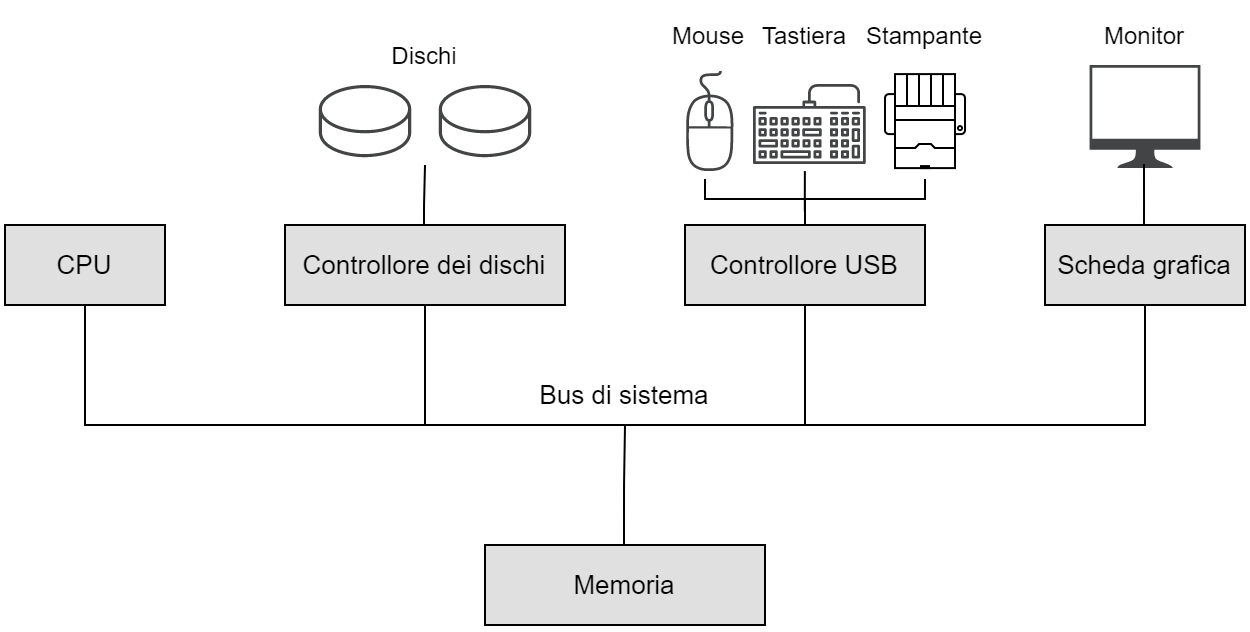
\includegraphics[width=0.9\textwidth]{img/img2.png}
        \caption{Un tipico sistema elaborativo}
        \label{fig:img2}
    \end{figure}
    
    Un moderno computer ha una o più (ma spesso più) CPU e un certo numero di controllori di dispositivi connessi attraverso un canale di comunicazione comune detto \textit{bus}, che permette l'accesso alla memoria condivisa del sistema.
    
    Il sistema operativo entra in gioco con i \textbf{driver del dispositivo}. Esso dispone di un driver per ogni controllore di dispositivo, che gestisce le specificità del controllore e funge da interfaccia con il resto del sistema.
    
    Andremo ora a descrivere in che modo il sistema operativo può garantire l'accesso concorrente e parallelo ai controllori, concentrandoci su tre aspetti chiave: interrupt, struttura della memoria e struttura I/O.
    
    \subsection{Interrupt}
        Un controllore che esegue un'operazione dovrà informare il sistema operativo, tramite il driver, di averla conclusa così da far eseguire le operazioni appropriate, come dare un output, restituire dati o semplicemente restituire il controllo. Come fa il controllore a comunicare al driver del dispositivo che ha terminato la sua operazione? Tramite un'\textbf{interruzione}, o \textit{interrupt}.
        
        
        \paragraph{Come una interrupt viene inviata.} Le \textbf{interruzioni} possono essere usate per vari scopi e costituiscono una componente chiave nell'interazione fra i sistemi operativi e l'hardware. Quest'ultimo può generare un'interruzione in qualsiasi momento inviando un segnale alla CPU, solitamente tramite il bus di sistema (un sistema di elaborazione può avere svariati bus, ma quello di sistema è il principale percorso di comunicazione fra i componenti fondamentali).
        
        \paragraph{Come una interrupt viene gestita.} Quando riceve una \textit{interrupt}, la CPU interrompe immediatamente l'elaborazione corrente, salva il suo stato e trasferisce l'esecuzione a una locazione fissa della memoria. Di solito questa locazione contiene l'indirizzo iniziale della procedura di servizio dell'interruzione. Una volta completata l'operazione, la CPU riprende qualsiasi operazione stesse eseguendo precedentemente.
        
        \paragraph{Come realizzare le interrupt.} Le interrupt sono un'operazione molto sensibile. Esse devono essere molto veloci, in quanto potrebbero avvenirne anche centinaia di volte al secondo. Un modo per realizzare ciò è creare una tabella di puntatori alle specifiche procedure richieste dalla interrupt, e memorizzarla in indirizzi di memoria bassi (per esempio i primi 100), così da potervi accedere direttamente senza operazioni intermedie. Molte funzioni riguardanti le interruzioni sono abbastanza comuni, basti pensare che sistemi operativi molto diversi come Windows e UNIX hanno lo stesso meccanismo di gestione delle interruzioni.
        
        \paragraph{Implementazione.}
            Il meccanismo alla base dell'implementazione della gestione delle interruzioni è piuttosto semplice. L'hardware disponde di un filo chiamato \textit{interrupt-request line} che la CPU controlla dopo l'esecuzione di ogni istruzione. Quando la CPU rileva un'interruzione la gestisce leggendone il numero di interruzione e saltando alla routine associata. Viene eseguito il salvataggio di informazioni che verranno modificate, l'elaborazione e il \texttt{return\textunderscore from\textunderscore interrupt} che ci riporta allo stato precedente.
            
            In altre parole il controllore del dispositivo \textit{solleva} un'interruzione, la CPU la \textit{intercetta} e la \textit{invia} al gestore delle interruzioni che a sua volta soddisfa la richiesta.
            
            Il meccanismo appena descritto è semplice ed efficace, ma in un sistema operativo moderno sono necessarie operazioni più sofisticate, come:
            \begin{enumerate}
                \item Possibilità di posticipare la gestione degli interrupt durante un'operazione critica.
                \item Metodo efficiente per inviare l'interruzione al gestore appropriato per un dato dispositivo.
                \item Interruzioni multilivello, con vari gradi di priorità.
            \end{enumerate}
            
            In un'architettura moderna queste tre funzioni sono fornite dalla CPU e dall'hardware del controllore delle interruzioni.
            
            La maggior parte delle CPU ha due linee di richiesta delle interruzioni: una viene detta \textbf{non mascherabile} (\textit{nonmaskable interrupt}) ed è riservata a eventi come errori irreversibili i memoria, mentre la seconda è \textbf{mascherabile} (\textit{maskable interrupt}), ovvero può essere disattivata dalla CPU prima dell'esecuzione di istruzioni critiche. L'interruzione mascherabile è quella usata dai controllori di dispositivi per richiedere un servizio.
            
    \newpage
    \subsection{Struttura della memoria}
        La memoria può essere ordinata in base a una gerarchia, che traccia un compromesso fra la capacità di archiviazione e il tempo di accesso; meno dati possono essere conservati sulla memoria, più velocemente è possibile accedervi. Infatti, per fare alcuni esempi, abbiamo in ordine dal meno capiente ma più veloce al più capiente ma meno veloce: registri, cache, dischi magnetici, etc...
        
        Un'altra distinzione importante è fra le memorie volatili e non volatili. Le prime perdono i dati immagazzinati quando viene tolta la fonte di energia che le alimenta, mentre le non volatili mantengono permanentemente i loro dati.
        
        In questo corso faremo riferimento alla memoria volatile come semplicemente \textbf{memoria}, mentre quella non volatile con l'acronimo \textbf{NVS}. Eventuali dispositivi specifici verranno specificati.
        
    \subsection{Struttura di I/O}
        Una cospicua parte di codice di un sistema operativo è dedicata alla gestione di I/O. Tutta via l'I/O guidato dalle interruzioni precedentemente descritto risulta poco efficace in alcuni casi, basti pensare al trasferimento di massicce quantità di dati da e verso NVS.
        
        La soluzione è l'\textbf{accesso diretto alla memoria} (\textbf{DMA}, o \textit{direct memory access}). Una volta impostati i buffer, i puntatori e i contatori necessari al dispositivo di I/O, il controllore spedisce un intero blocco dati dal proprio buffer alla memoria centrale, senza intervento della CPU, richiedendo così una interrupt per ogni blocco dati anziché per ogni byte.
    
\section{Architettura degli elaboratori}
    \subsection{Sistemi monoprocessore e multiprocessore}
            Per sistema monoprocessore intendiamo un qualsiasi sistema con un solo core. Un sistema potrebbe avere microprocessori specializzati, come per esempio un microprocessore nella tastiera che individua e comunica la pressione esercitata sui tasti, ma questo non rende un sistema multiprocessore.
            
            Pochissimi computer moderni sono monoprocessore. Nel panorama moderno i sistemi multiprocessore sono l'alternativa più diffusa. Un tale sistema dispone di due o più processori, ognuno dotato di una singola unità di calcolo. Il vantaggio è di ottenere una maggiore capacità elaborativa (\textit{throughput}). Tuttavia aumentando di \textit{N} volte il numero di core, non aumenta di \textit{N} volte la capacità di elaborazione, siccome è necessario del lavoro supplementare (\textit{overhead}) per garantire che tutti i componenti funzionino correttamente.
            
            La modalità più diffusa di elaborazione parallela è la \textbf{SMP}, o \textbf{multielaborazione simmetrica}, in cui ogni processore, alla pari degli altri, è abilitato all'esecuzione di tutte le funzioni del sistema.
            
            \begin{figure}[h]
                \centering
                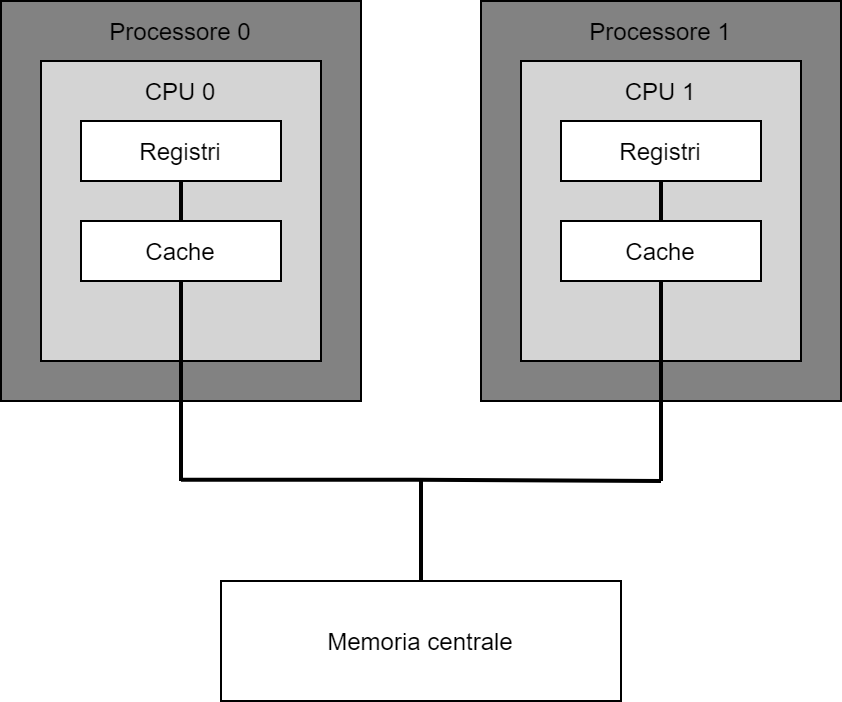
\includegraphics[width=0.85\textwidth]{img/img3.png}
                \caption{Architettura di multielaborazione simmetrica}
                \label{fig:img3}
            \end{figure}
            
            \newpage
            Nonostante ogni core abbia un suo set di registri e una cache privata, condividono la memoria fisica sullo stesso bus di sistema.
            
            Il vantaggio di questo tipo di sistema è che per \textit{N} processori, \textit{N} processi possono essere eseguiti contemporaneamente senza un rilevante calo delle prestazioni. Tuttavia potrebbe capitare che un processore è in sovraccarico, mentre l'altro è totalmente inattivo. Questo potrebbe essere risolto permettendo ai processori di condividere alcune strutture dati, ma come vedremo in futuro, ciò va implementato con molta attenzione.
            
            La definizione di \textbf{multiproccessore} si è evoluta col tempo e oggi include sistemi in cui più CPU risiedono in un singolo chip. Questo è conveniente da un punto di vista computazionale in quanto lo scambio di dati all'interno di uno stesso chip è più veloce di uno scambio fra chip diversi. Inoltre un chip richiede una potenza minore per essere alimentato, cosa molto utile nei sistemi a batteria come smartphone e laptop.
            
            Questo ultimo stile di architettura è il più utilizzato e oltre a considerazioni su condivisione della memoria, delle risorse e accessi, al sistema operativo queste CPU multicore appaiono come \textit{N} normali processori.
            
            \subsubsection{Cluster di elaboratori}
                I \textit{clustered systems} o semplicemente \textbf{cluster} sono un tipo di sistemi multiprocessore, ma anziché essere basati su più CPU, sono basati su più calcolatori completi (debolmente accoppiati), detti nodi, collegati fra loro.
                
                Alcuni dei vantaggi di un sistema del genere sono l'\textbf{elevata disponibilità}, che permette di mantenere operativo il cluster anche se un calcolatore si guasta, il \textbf{degrado controllato}, che permette di fornire una qualità del servizio proporzionale al numero di calcolatori operativi, che in alcuni casi si spingono oltre e formano sistemi \textbf{tolleranti ai guasti} (\textit{fault tolerant}), che permettono addirittura il funzionamento normale del sistema nonostante il guasto di un nodo.
                
                Un tipo di sistemi che si basano su cluster sono quelli ad alte prestazioni, che però hanno bisogno di una tecnica chiamata \textbf{parallelizzazione}, che suddivide il programma in componenti separate, permettendo così l'elaborazione di queste singole componenti sui vari nodi. Una cosa che vediamo nei cluster è l'accesso condiviso alla memoria. Abbiamo così nodi che comunicano fra di loro, sono \textit{loosely coupled} ed accedono alla stessa memoria, fornendo sistemi estremamente resistenti, stabili, efficienti e flessibili.
                
\section{Attività del sistema operativo}
    Avendo passato in rassegna organizzazione e struttura dei sistemi informatici, siamo pronti ad affrontare i sistemi operativi. Il sistema operativo costituisce l'ambiente di esecuzione dei programmi. La struttura dei vari sistemi operativi può cambiare molto, ma ci sono alcuni aspetti comuni di cui andiamo a parlare.
            
    Durante l'avvio e il riavvio di un calcolatore, c'è bisogno di un \textbf{programma di avviamento} detto \textit{bootstrap program}, che è piuttosto semplice e spesso memorizzato nel \textit{firmware} che fa parte dell'hardware. Il suo compito è inizializzare le varie componenti come registri, memoria centrale, etc. Deve inoltre caricare il sistema operativo e avviarne l'esecuzione; a tale scopo deve caricare il kernel del sistema operativo.
    Una volta caricato e in esecuzione il kernel può iniziare a offrire servizi. Tuttavia alcuni servizi vengono offerti da programmi di sistema caricati durante l'avviamento. Questi \textbf{processi di sistema} o \textit{daemons}, restano in esecuzione per tutto il tempo per cui è in esecuzione il kernel. In Linux il primo daemon avviato è \texttt{systemd}, che a sua volta avvia diversi altri daemons.
            
    Una volta che questa fase è completata il sistema è pronto per essere utilizzato e attende che si verifichi qualche evento. Se nessun evento avviene e se i dispositivi di I/O non richiedono alcun servizio il sistema operativo resta in \textit{idle}, termine che non ha un corrispettivo italiano ma potrebbe essere grezzamente tradotto con \textbf{girarsi i pollici}.
            
    Un evento è quasi sempre segnalato da un'interruzione. Abbiamo precedentemente descritto le interruzioni hardware, ma un altro tipo di interruzioni è data dalle eccezioni (\textbf{trap} o \textbf{exception}) ossia interruzioni generate dal software causate da un errore o dalla richiesta di erogazione da parte di un programma utente di uno dei servizi del sistema operativo, realizzata tramite l'esecuzione di un'operazione detta \textbf{chiamata di sistema} (\textit{system call}).
            
    \subsection{Multiprogrammazione}
        Una caratteristica principale dei sistemi operativi è il supporto della \textbf{multiprogrammazione}. Un singolo programma non è in grado di tenere occupata in maniera costante CPU e dispositivi I/O. Inoltre, con grande probabilità un utente vorrà eseguire più programmi contemporaneamente. La multiprogrammazione risolve tutti questi problemi, aumentando la percentuale di utilizzo della CPU organizzando i programmi in esecuzione (chiamati \textbf{processi} in un ambiente di multiprogrammazione) in maniera tale da tenerla costantemente occupata.
                
        L'idea fondamentale è questa: la CPU ha in memoria centrale una serie di processi che devono essere eseguiti. Inizia ad eseguirne uno, ma questo dovrebbe prima o poi trovarsi ad attendere (per esempio per una lenta operazione di I/O). La CPU sfrutta questo tempo di idle per passare al prossimo processo ed eseguirlo. Finché la lista di processi da eseguire ha anche solo un elemento, la CPU non sarà inattiva.
            
        Il \textbf{multitasking} è un'estensione logica della multiprogrammazione: la CPU esegue più lavori commutando le loro esecuzioni con una velocità tale da permettere a tutti gli utenti di usufruire di tempi di risposta rapidi. Riguardo queste due caratteristiche ci sono dei ragionamenti da fare, relativi a scheduling della CPU, problemi legati alla memoria e sicurezza, che verranno discussi in futuro.
                
    \subsection{Duplice modalità di funzionamento}
        Uno dei compiti del sistema operativo è quello di assicurarsi che un utente non svolga (volontariamente o meno) azioni dannose per il sistema o per altri utenti. Questo può essere assicurato definendo due modalità operative, una detta \textbf{modalità utente} e l'altra \textbf{modalità di sistema} (o modalità \textit{kernel}, \textit{supervisore}, \textit{monitor} o \textit{privilegiata}). La selezione fra queste modalità avviene tramite un bit, e il controllo viene passato quando necessario. Per esempio se un programma utente richiede una funzione del sistema operativo, passa il controllo, il sistema operativo esegue tale funzione e ripassa il controllo all'utente.
                
        \begin{figure}[h]
            \centering
            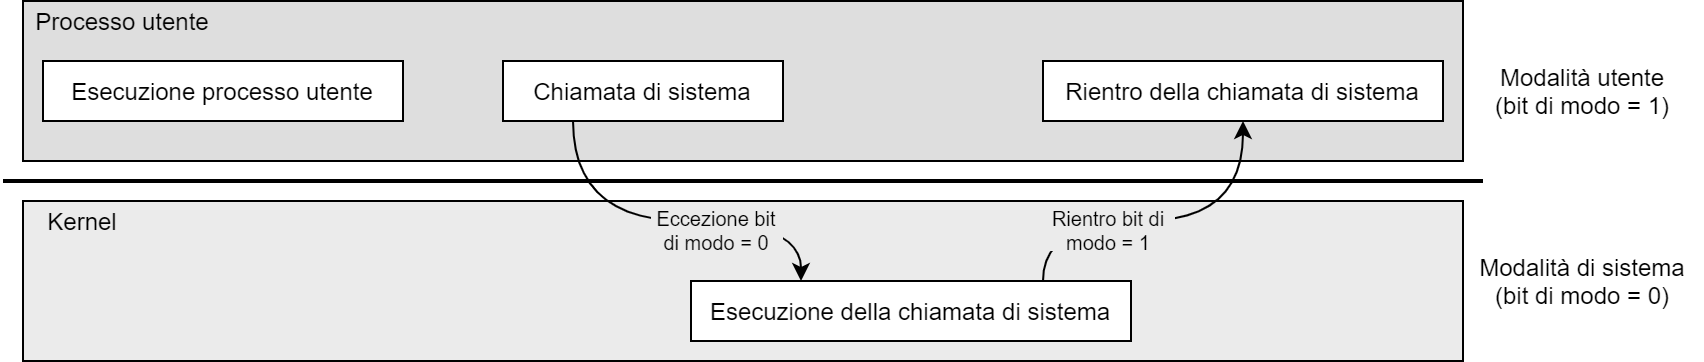
\includegraphics[width=1\textwidth]{img/img4.png}
            \caption{Transazione da modalità utente a modalità di sistema.}
            \label{fig:img4}
        \end{figure}
                
        Questa \textit{dual mode} garantisce anche la sicurezza del sistema nei confronti di operazioni dannose, in quanto vengono definite delle \textbf{istruzioni privilegiate} eseguibili solo in modalità di sistema, modalità a cui ovviamente l'utente non può fare accesso liberamente.
                
        Possono esserci anche più di due livelli, e infatti molti sistemi ne hanno di più.
                
    \subsection{Timer}
        Il \textbf{timer} è il modo che ha il sistema operativo per mantenere il controllo della CPU. Abbiamo un timer programmabile affinché invii un segnale d'interruzione a intervalli di tempo specificati, che possono essere fissi o variabili. Prima di restituire all'utente il controllo dell'esecuzione, il sistema operativo assegna un valore al timer. Allo scadere di questo valore genera un'interruzione che causa il trasferimento del controllo al sistema operativo, che potrà decidere se lasciare altro tempo al programma o interpretare l'interruzione come un errore fatale. Ovviamente, le istruzioni di controllo del timer sono eseguibili solo in modalità privilegiata.
                
\section{Gestione delle risorse}
    Come abbiamo già accennato il sistema operativo può essere visto come un gestore di risorse. Andiamo a vedere ora come gestisce tali risorse.
    
    \subsection{Gestione dei processi}
        Abbiamo già visto il concetto di processo. Un processo può eseguire una serie di compiti, ma per ora lo consideriamo come un lavoro d'elaborazione (\textit{job}) eseguito in un ambiente time-sharing, anche se il concetto è più generale.
        
        Il compito di gestire le risorse usate dei processi ce l'ha il sistema operativo, che può assegnarne alla creazione del processo o in maniera dinamica durante la sua esecuzione.
        
        C'è da specificare che un programma di per sé è un'entità passiva, mentre il processo è un'entità attiva. Un processo a singolo \textit{thread} ha un'esecuzione sequenziale; ha una serie di istruzioni che vengono eseguite una dopo l'altra. Un \textbf{contatore di programma} tiene il conto della prossima istruzione da eseguire, e anche se due processi appartengono allo stesso programma si considerano due sequenze di istruzioni separate. Un processo multithread ha più contatori di programma, ognuno dei quali punta all'istruzione da eseguire per il dato thread.
        
        Il processo è l'unità di lavoro di un sistema, e infatti il sistema può essere visto come un insieme di processi (alcuni eseguono codice del sistema, altri codice utente), che possono potenzialmente essere eseguiti in modo concorrente. Il sistema operativo ha la responsabilità di eseguire le seguenti attività connesse alla gestione dei processi:
        \begin{itemize}
            \item Creazione e cancellazione di processi utente e di sistema.
            \item Scheduling di processi e thread sulle CPU.
            \item Sospensione e ripristino dei processi.
            \item Fornitura di meccanismi per la sincronizzazione dei processi.
            \item Fornitura di meccanismi per la comunicazione fra processi.
        \end{itemize}
        
    \subsection{Gestione della memoria}
        La memoria centrale è un vasto vettore che può contenere fino a miliardi di parole, ognuna con il suo indirizzo. Generalmente è l'unico grande dispositivo di memorizzazione a cui la CPU può far riferimento e accedere in modo diretto.
        
        I sistemi moderni devono tenere in memoria molti programmi e dati, e la maniera in cui ottimizzano questo compito dipende dallo schema di gestione utilizzato, che può variare di efficacia in base a molti fattori, fra cui il tipo di architettura hardware del sistema.
        
        Il sistema operativo è responsabile di tenere traccia di quali parti di memoria sono attualmente in uso e da chi, di assegnare e revocare lo spazio di memoria secondo necessità, e infine di decidere quali processi (o parti di essi) e dati debbano essere caricati in memoria centrale o trasferiti nella memoria di massa.
        
    \subsection{Gestione dei file}
        Il sistema operativo definisce un'unità logica di archiviazione allo scopo di dare un'interfaccia chiara e uniforme, nella forma del \textbf{file}. Questo concetto è uno dei più visibili del sistema operativo, ma anche uno dei più generali; un file può avere vari formati, da molto liberi, ad eseguibili, a rigidamente formattati, come un file MP3.
        
        I file possono essere organizzati in directories per facilitarne la gestione, e inoltre se diversi utenti utilizzano il sistema potrebbe essere desiderabile controllare chi ha accesso a un determinato file.
        
        Il sistema operativo è responsabile delle seguenti attività connesse alla gestione dei file:
        \begin{itemize}
            \item Creazione e cancellazione dei file.
            \item Creazione e cancellazione delle directory.
            \item Fornire le funzioni fondamentali per la gestione di file e directory.
            \item Associazione di file a dispositivi di memoria secondaria.
            \item Creazione di backup di file su dispositivi di memoria non volatili.x
        \end{itemize}
        
    \subsection{Gestione della memoria di massa}
        La maggior parte dei sistemi operativi moderni usa memorie secondarie, spesso dischi magnetici o NVM, per immagazzinare dati e programmi (sono usati sia come sorgente che come destinazione dei dati creati). Il sistema operativo è responsabile delle seguenti attività connesse alla memoria di massa:
        \begin{itemize}
            \item Montare (\textit{mounting}) e smontare (\textit{unmounting}) le unità di memoria.
            \item Gestione dello spazio libero.
            \item Assegnazione dello spazio.
            \item Sceduling del disco.
            \item Partizionamento.
            \item Protezione.
        \end{itemize}
        
        La natura di questo tipo di memoria può variare in base all'uso che si intende farne. A volte potrebbe essere desiderabile un dispositivo più capiente ma più lento.
        
        Un altro tipo di memoria da citare è la \textbf{memoria terziaria}, composta da CD-ROM, chiavette USB, eccetera. Il sistema potrebbe decidere di gestire direttamente questi dispositivi come di delegarne la gestione a programmi applicativi.
        
    \subsection{Gestione della cache}
        Questo è un concetto importante di un sistema elaborativo. Solitamente le informazioni sono mantenute in memoria centrale, e al momento del loro utilizzo si copiano in un'unità più veloce, la \textbf{cache} appunto.
        
        Quando si deve utilizzare un'informazione si controlla se è presente nella cache e nel caso si usa quella copia, altrimenti si esegue una copia e la si mantiene in cache, sulla supposizione che presto servirà nuovamente.
        
        Data la limitata capacità della cache, la sua gestione è un importante problema di progettazione. Per esempio una questione molto delicata è quella delle multiple copia di un singolo oggetto; avendo vari tipi di memoria disposti in maniera gerarchica, un dato potrebbe essere in più di queste memorie contemporaneamente. Dobbiamo assicurarci, nel caso di un sistema multiprocessore, che venga presa la versione di questo dato aggiornata più di recente. La questione diventa ancora più delicata quando abbiamo più CPU, in quanto ogni CPU ha una sua cache locale, e i dati fra queste varie cache devono essere coerenti, dando vita appunto al problema della \textbf{coerenza della cache}, e che solitamente si risolve a livello di hardware, lasciando fuori quindi il sistema operativo. Andando a disperdere ancora di più i dati, quindi in sistemi distribuiti, la questione della coerenza diventa ancora più delicata, facendo sorgere la necessità di mantenere la coerenza del dato fra calcolatori diversi, i quali si trovano potenzialmente in locazioni geografiche disparate.
        
    \subsection{Gestione dell'I/O}
        Un compito del sistema operativo è quello di nascondere agli utenti le peculiarità dei vari dispositivi. In UNIX, per esempio, le caratteristiche dei dispositivi di I/O sono nascoste alla maggior parte dello stesso sistema operativo dal \textbf{sottosistema di I/O}, che è composto dalle seguenti parti:
        
        \begin{itemize}
            \item Un componente di gestione della memoria, fra cui gestione di buffer di I/O, gestione della cache e gestione delle aree di memoria per l'I/O asincrono (\textit{spooling}).
            \item Un'interfaccia generale per i driver dei dispositivi.
            \item I driver per gli specifici dispositivi.
        \end{itemize}
        
        Solo il driver del dispositivo conosce le peculiarità del dispositivo cui è assegnato.
        
\section{Virtualizzazione}
    La \textbf{virtualizzazione} è una tecnica che permette di astrarre l'hardware di un singolo computer (CPU, memoria, etc.) in diversi ambienti di esecuzione, creando così l'illusione che ogni distinto ambiente sia in esecuzione sul proprio computer. Un utente di una cosiddetta \textbf{macchina virtuale} può passare da un sistema operativo a un altro esattamente come in una situazione normale passa tra processi di esecuzione in un singolo sistema operativo.
    
    La virtualizzazione permette quindi a interi sistemi operativi di funzionare come fossero applicazioni all'interno di altri sistemi operativi. Questo fa parte di una tipologia di software che include l'\textbf{emulazione}, la quale tende a essere meno performante, soprattutto se le prestazioni della CPU emulatrice e quella emulata sono simili, in quanto ogni singola istruzione della CPU emulata deve essere replicata.
    
    Abbiamo due tipi di virtualizzazione:
    \begin{itemize}
        \item \textbf{Full virtualization:} Emula ogni cosa, fino alle istruzioni assembler.
        \item \textbf{Para-virtualization:} Prevede che ci sia una macchina in un dominio privilegiato \texttt{dom0} e tanti sistemi in altri domini che per eseguire proessi usano i servizi della macchina in \texttt{dom0}.
    \end{itemize}

\chapter{Parte Prima, Capitolo 2: Strutture dei Sistemi Operativi}
\section{Servizi di un Sistema Operativo}
    Un sistema operativo fornisce un ambiente in cui eseguire programmi e fornire servizi, che possono variare in base allo specifico sistema operativo, ma possiamo riconoscere alcune classi comuni di servizi.
    
    \subsection{Funzionalità utili all'utente}
        Un primo insieme di servizi offre funzionalità utili all'utente.
        
        \paragraph{Interfaccia con l'utente.} O UI, può assumere diverse forme. La più comune consiste di un'interfaccia a finestre con un puntatore e un input testuale, ma per dispositivi come tablet e smartphone possiamo avere touch screen con relativi metodi di interazione. Possiamo anche avere un'interfaccia a linea di comando (CLI).
        
        \paragraph{Esecuzione di un programma.} Un sistema operativo deve permettere di caricare in memoria ed eseguire un programma. Deve anche poter terminare l'esecuzione in maniera corretta o anomala (segnalando quest'ultimo caso).
        
        \paragraph{Operazioni di I/O.} Un programma in esecuzione dovrebbe poter richiedere operazioni di I/O, che per alcuni dispositivi potrebbero richiedere funzioni particolari. Inoltre per motivi di efficienza e protezione, l'utente non può controllare direttamente questi dispositivi, quindi il sistema operativo deve mettere a disposizione strumenti adeguati per la loro gestione.
        
        \paragraph{Gestione del file system.} I programmi richiedono l'esecuzione di operazioni di lettura e scrittura su file, possono modificarli, cercarli o cancellarli, oltre che gestire directory. Alcuni sistemi forniscono tutte o alcune di queste operazioni in base alla proprietà dello stesso, mentre molti sistemi operativi fanno scegliere all'utente diversi file system con funzionalità e prestazioni specifiche.
        
        \paragraph{Comunicazioni.} Spesso un processo ha bisogno di scambiare informazioni con un altro processo in esecuzione. Questo può avvenire fra processi sullo stesso calcolatore o attraverso la rete. Questo scambio può avvenire tramite una \textbf{memoria condivisa}, che permette a entrambi di leggere e scrivere in una porzione di memoria che condividono, o attraverso lo \textbf{scambio di messaggi}, cosa gestita dal sistema operativo.
        
        \paragraph{Rilevamento di errori.} Il sistema operativo deve essere capace di gestire diversi tipi di errore, come un fallimento dell'hardware, un problema nei dispositivi di I/O o nei programmi utente. A volte l'unico modo di gestire correttamente queste situazioni è arrestare il sistema, mentre altre volte potrebbe essere necessario solo arrestare il processo colpevole o inviare un messaggio di errore.
        
    \subsection{Funzioni utili al sistema}
        Un secondo insieme comprende funzioni che assicurano il corretto funzionamento del sistema, anche se non sono direttamente rilevate dall'utente.
        
        \paragraph{Allocazione delle risorse.} Se più utenti usano la stessa macchina (situazione ormai rara) o più processi sono in esecuzione contemporaneamente, è compito del sistema operativo gestire le risorse in modo che nessun processo monopolizzi la potenza computazionale e nessuno muoia per mancanza di risorse.
        
        \paragraph{Logging.} È in pratica il mantenere traccia di quali programmi o processi consumano quante risorse, e altre informazioni affini. Questo può servire per una serie di cose, fra cui compilare statistiche che possono essere utili a una futura gestione più efficiente del sistema.
        
        \paragraph{Protezione e sicurezza.} La \textbf{protezione} assicura che l'accesso alle risorse del sistema sia controllato, in maniera che nessun estraneo possa accedervi. La \textbf{sicurezza} inizia dalla richiesta di autenticazione e si espande fino al controllo di accessi maligni tramite dispositivi di I/O. Un sistema protetto e sicuro deve porre precauzioni ovunque, in quanto la forza di una catena è solo quella del suo anello più debole.
        
\section{System Calls (chiamate di sistema)}
    Le chiamate di sistema rappresentano un'interfaccia per i servizi resi disponibili dal sistema operativo. Esse sono il principale metodo di interazione fra i programmi utenti e il kernel, in quanto spesso vengono usate durante la modalità utente per richiedere servizi disponibili solo in modalità kernel.
    
    I programmatori spesso non accedono direttamente nemmeno alle system calls, ma hanno a disposizione una \textbf{API} (\textit{application programming interface}), che varia da sistema a sistema (Windows ha le sue API, mentre i sistemi basati sullo standard POSIX, il che comprende praticamente tutti i sistemi UNIX, Linux e macOS, hanno la loro per esempio), e che chiama le system calls corrette richieste dall'utente. Ci sono una serie di ragioni per cui uno sviluppatore potrebbe preferire l'utilizzo delle API, come per esempio rendere l'applicazione portabile su tutti i sistemi operativi che operano sullo stesso standard.
    
    Le system calls vengono richiamate tramite un codice identificativo unico per ognuna e sono memorizzate in una tabella.
    
    \subsection{Categorie di system calls}
        Le system calls possono essere classificabili in approssimativamente sei categorie, che andremo di seguito a descrivere.
        
        \paragraph{Controllo dei processi.} Ci sono molti punti di vista sotto cui i processi devono essere gestiti; la loro interruzione per esempio, può essere regolare o anomala, e un'interruzione non andata a buon fine ha diversi livelli di gravità (possiamo generalizzare il concetto dicendo che un'interruzione andata a buon fine ha livello di gravità 0). Quando un processo viene terminato in maniera anomala potremmo voler analizzare dati relativi alla sua terminazione.
        
        Un'altra caratteristica dei processi è ovviamente la loro creazione, quante risorse consuma e per quanto tempo viene eseguito. Inoltre, in un processore multitask abbiamo bisogno di gestire il parallelismo, schedulando l'esecuzione e l'arresto dei vari processi in base alla disponibilità del processore.
        
        Tutte queste operazioni vengono gestite tramite chiamate di sistema.
        
        \paragraph{Gestione dei file.} In base al file system devono essere rese disponibili determinate operazioni sui file, fra cui creazione, rimozione, apertura, lettura, scrittura, chiusura, eccetera. Le stesse operazioni, nel caso in cui il file system sia strutturato in directories, devono essere disponibili anche sulle suddette. Il sistema operativo potrebbe rendere disponibili queste operazioni tramite chiamate di sistema, interfacce grafiche, programmi, etc.
        
        \paragraph{Gestione dei dispositivi.} L'assegnamento e in generale la gestione delle risorse avviene spesso tramite dispositivi: la memoria viene assegnata tramite il disco, la potenza di calcolo tramite il processore, le elaborazioni grafiche tramite la GPU, etc.
        
        È quindi ovvio che c'è bisogno di un modo per gestire questi dispositivi. Questi devono essere, nel caso di un sistema multiutente per esempio, assegnati talvolta a un utente in maniera esclusiva, inizializzati, chiusi quando necessario. Queste operazioni possono essere viste come simili a quelle eseguite sui file, e difatti alcuni sistema operativi, come Linux, uniscono la gestione dei file e dei dispositivi in un unico sistema file-dispositivi.
        
        \paragraph{Gestione delle informazioni.} Una buona parte delle chiamate di sistema serve a scambiare informazioni fra il sistema e l'utente. Ci sono molte informazioni che l'utente potrebbe voler recuperare dal sistema, come la data, l'ora, o informazioni specifiche sulla memoria. O ancora, informazioni sui processi, di cui il sistema tiene traccia in maniera dettagliata, descrivendone per esempio il tempo di esecuzione e le risorse utilizzate.
        
        \paragraph{Comunicazione.} Ci sono due metodi molto diffusi di scambio di messaggi fra processi. Il primo è il \textbf{modello a messaggi}, che prevede lo scambio di messaggi sia in maniera diretta che indiretta, tramite l'utilizzo di una \textit{mailbox} comune. Il processo che fornisce il messaggio si chiama \textit{client}, mentre quello che lo riceve si chiama \textit{server}.
        
        L'altro metodo per scambiare i messaggi è usare una \textbf{memoria condivisa}, che prevede la lettura e la scrittura da parte di due processi sulla stessa memoria, con la condizione di evitare conflitti (non scrivere contemporaneamente). Questo avviene per esempio con i \textit{thread}.
        
        Lo scambio di messaggi è preferibile quando vanno scambiate piccole quantità di informazioni e quando i due processi esistono su calcolatori distinti, per esempio che comunicano tramite la rete, mentre l'accesso condiviso alla memoria permette la massima velocità ed è quindi preferibile per grandi scambi di dati.
        
        \paragraph{Protezione.} Storicamente era necessario tenere in considerazione la protezione su sistemi che prevedevano l'utilizzo da parte di molti utenti, ma oggi, con l'accesso di ogni dispositivo a Internet, è necessario prendere sempre in considerazione la protezione.
        
        Il sistema operativo può chiedere i permessi e l'autenticazione all'utente e di conseguenza permettere o negare l'accesso.
        
\section{Struttura del sistema operativo}
    Allo scopo di far funzionare correttamente un sistema complesso come un sistema operativo moderno e di non renderne impossibile la manutenzione, è necessario strutturarne le componenti in maniera studiata. Un metodo di strutturazione è quello \textbf{monolitico}, che tuttavia col tempo è stato abbandonato in favore di una struttura \textbf{modulare}, che prevede la presenza di moduli con interfacce ben definite.
    
    \subsection{Struttura monolitica}
        Il modo più semplice di strutturare un sistema operativo è tramite l'assenza di struttura, ossia mettendo tutte le funzionalità del kernel in un unico file binario che viene eseguito una volta all'interno di un unico spazio di indirizzamento. Abbiamo per esempio il sistema operativo UNIX originale, che consta di due parti: il kernel e i programmi di sistema. Un sistema così strutturato è difficile da gestire, ma ottiene un vantaggio in termini di prestazioni in quanto il grande numero di servizi e funzioni eseguite all'interno del kernel implicano un overhead ridotto, e ciò giustifica alcuni elementi di questo tipo di struttura all'interno dei sistemi operativi moderni.
        
    \subsection{Approccio stratificato}
        I sistemi monolitici vengono anche chiamati \textbf{strettamente accoppiati} (\textit{tightly coupled}), in quanto ogni parte del kernel è dipendente da ogni altra parte. In alternativa possiamo pensare di strutturare il sistema con in mente un \textbf{basso accoppiamento} (\textit{loosely coupled}), il che ci permette di modificare un modulo senza andare necessariamente sugli altri.
        
        Un modo di rendere modulare un sistema operativo è tramite la \textbf{stratificazione}. In un tale sistema, gli strati più bassi rappresentano l'hardware, mentre quelli più alti l'interfaccia utente. 
        
        \begin{figure}
            \centering
            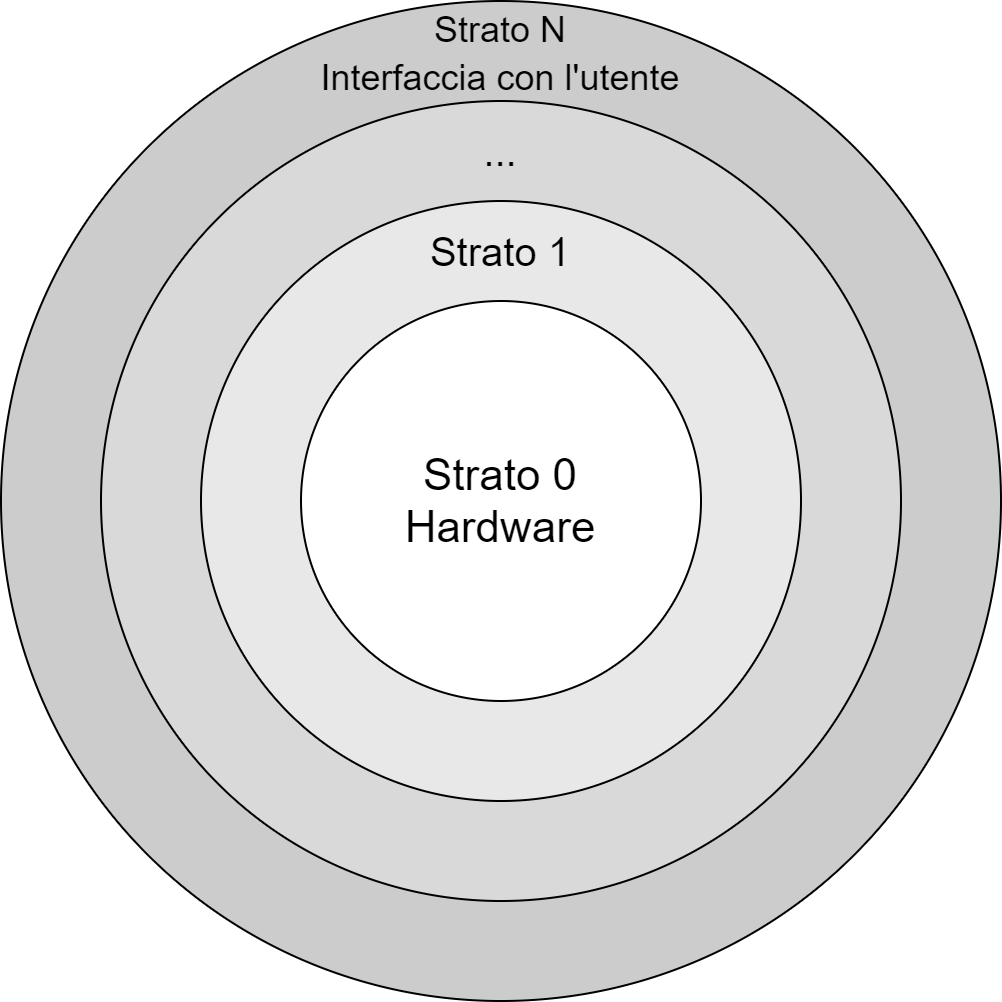
\includegraphics[width=0.5\textwidth]{img/img5.png}
            \caption{Struttura a strati di un sistema operativo.}
            \label{fig:img5}
        \end{figure}
        
        C'è da dire che recentemente si sono aggiunti strati addirittura superiori all'interfaccia utente. Pensiamo per esempio alle macchine virtuali, che hanno i loro strati, tutti superiori all'interfaccia utente, e forniscono anche loro un'interfaccia utente.
        
        Il funzionamento degli strati è opaco. Uno strato fornisce servizi allo strato superiore, e può richiederne a quello direttamente inferiore. Questo tipo di struttura rende relativamente facile la progettazione, in quanto possiamo sviluppare uno strato dando per scontato che quelli inferiori siano stati correttamente testati e usando le funzioni che ci mettono a disposizione. Questo metodo viene usato con successo per esempio nella costruzione di applicazioni web, ma raramente un approccio a stati puro viene osservato in un sistema operativo, in quanto è difficile definire le operazioni di un dato strato, e le prestazioni ne soffrono molto.
        
        La soluzione adottata spesso dai sistemi operativi moderni è un approccio ibrido, in cui abbiamo pochi strati con più funzioni nel singolo strato.
        
    \subsection{Microkernel}
        Come abbiamo visto in precedenza, il sistema operativo UNIX, in funzione della sua struttura monolitica, tendeva a crescere sempre di più, diventando sempre più difficile da gestire.
        
        Verso la metà degli anni '80 fu sviluppato il sistema operativo \textbf{Mach}, con il kernel strutturato in moduli secondo il cosiddetto orientamento a \textbf{microkernel}. La filosofia dietro questo tipo di strutturazione è quella di rimuovere dal kernel tutte le funzioni non strettamente necessarie, fornendole come programmi di livello utente e di sistema. Non c'è un consenso comune su quali servizi siano strettamente necessari, ma in generale un microkernel offre i servizi minimi di gestione dei processi, della memoria e della comunicazione. Ne risulta un microkernel di dimensioni molto ridotte e più facile da gestire a causa del grado di modularità introdotto.
        
        Lo scopo principale di un microkernel è quello di fornire funzioni di comunicazione fra i programmi client e i vari servizi, comunicazione che avviene tramite messaggi.
        
        Ovviamente un kernel di questo tipo è molto più facile da gestire, espandere ed è inoltre più sicuro, in quanto la compromissione di un servizio avviene spesso nello spazio utente, lasciando al sicuro le funzioni core del sistema operativo.
        
        Lo svantaggio è che i microkernel possono incorrere in cali di prestazioni, principalmente dovuto a un maggiore overhead causato dalla necessità di far comunicare due o più processi in spazi di indirizzamento diversi.
        
    \subsection{Moduli}
        Forse il miglior metodo attualmente disponibile per la progettazione di sistemi operativi si basa sull'utilizzo di \textbf{moduli del kernel caricabili dinamicamente}. In questo contesto il kernel è costituito da una serie di componenti di base che vengono poi integrati da funzionalità caricate dinamicamente all'avvio o durante l'esecuzione per mezzo di moduli. Molte implementazioni moderne di UNIX, come Linux, macOS e Solaris, come anche Windows, usano questo metodo.
        
        L'idea è che il kernel debba fornire alcuni servizi principali e offrire gli altri servizi in maniera dinamica, senza tuttavia aggiungerli direttamente al kernel, in quanto ciò richiederebbe una ricompilazione.
        
        Il risultato finale ricorda un sistema a strati, in quanto diverse sezioni del kernel offrono servizi ben distinti, ma ha una maggiore flessibilità (è meno opaco) in quanto ogni modulo può richiamare ogni altro modulo. Ricorda per certi versi anche l'approccio a microkernel, in quanto la parte principale del kernel implementa solo le funzioni di base, ma è più efficiente siccome i moduli caricati dinamicamente non devono comunicare tramite messaggi.
        
        Linux implementa un sistema di LKM, \textit{loadable kernel module}, principalmente per caricare driver di dispositivi e file system.
        
\section{Linker e Loader}
    Generalmente un programma risiede su un disco in forma di un file binario eseguibile. Per essere eseguito su una CPU, il programma deve essere caricato in memoria e inserito nel contesto di un processo.
    
    Innanzitutto i file sorgente vengono compilati in file oggetto progettati per essere ricaricati in qualsiasi locazione della memoria, e sono chiamati \textbf{file oggetto rilocabili}. In seguito, il \textit{linker} combinai file oggetto rilocabili in un singolo file binario eseguibile.
    
    Durante la fase di \textbf{linking}, possono essere inclusi altri file oggetto o librerie, dando a questa fase una natura che si presta a una certa modularità.
    
    Per caricare il file eseguibile in memoria, dove diventa idoneo e disponibile all'esecuzione, viene usato un \textbf{loader}. Una fase del caricamento è la rilocazione, la quale ha il compito di assegnare le locazioni di memoria definitive al programma, in modo da poter, per esempio, trovare le variabili globali e accedere alle funzioni di libreria.
    
    Ci sono molti standard per questo tipo di file, per esempio in ambiente Linux abbiamo il formato \textbf{ELF}, ossia Executable and Linkable Format. Oltre al codice macchina compilato e metadati relativi a simboli e funzioni, questo contiene anche un \textit{entry point}, che è semplicemente la prima istruzione da eseguire.

\chapter{Parte Seconda, Capitolo 3: Processi}
In origine era permessa l'esecuzione di un solo programma per macchina, il quale aveva il controllo totale della suddetta.

Ma oggi possiamo avviare potenzialmente centinaia di programmi contemporaneamente ed essi possono operare con un certo grado di indipendenza.

Ciò è possibile grazie al concetto di \textit{processo}, ossia ciò che in prima istanza definiamo come un programma in esecuzione, o, l'unità di lavoro dell'elaboratore.

Con la crescente complessità dei sistemi, cresce anche la necessità di gestione dei processi. Infatti, oltre ai programmi utente c'è anche necessità di gestire processi di sistema.

Un sistema è dunque composto da un insieme di processi: quelli del sistema operativo che eseguono il codice di sistema, e quelli utente che eseguono il codice utente.

\section{Concetto di Processo}
    La necessità di dare un nome al lavoro eseguito dalla CPU c'è sempre stato, e sono stati usati termini come \textit{task}, \textit{job}, eccetera. Anche un sistema monoutente esegue spesso multipli programmi, e anche nel caso dell'esecuzione di un singolo programma, ha bisogno di gestire una serie di attività interne. Queste unità di lavoro prendono comunemente il nome di \textbf{processi}.
    
    C'è da ricordare che in alcuni casi potrebbe essere usato il termine ormai superato \textit{job}, nel caso di terminologie ben stabilite come \textit{job scheduling}.
    
    \subsection{Il Processo}
        Lo stato dell'attività corrente di un processo è rappresentato dal valore del contatore di programma. La sua struttura interna è divisa in sezioni come descritto in figura.
        
        \begin{figure}[h]
            \centering
            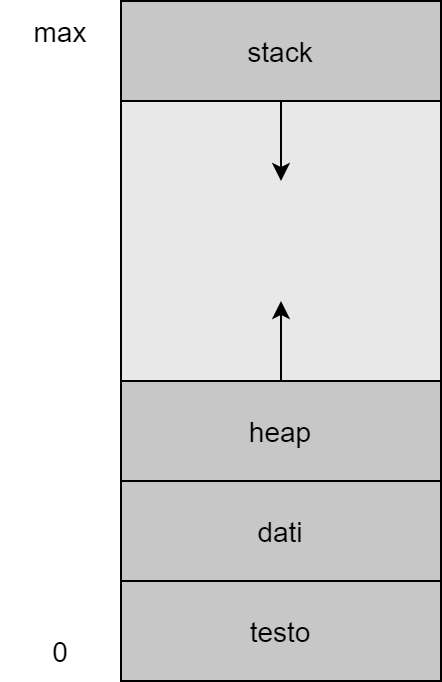
\includegraphics[width=0.3\textwidth]{img/img6.png}
            \caption{Struttura di un processo in memoria}
            \label{fig:img6}
        \end{figure}
        
        Le sezioni sono le seguenti:
        \begin{itemize}
            \item \textbf{Sezione di testo:} Contiene il codice eseguibile.
            \item \textbf{Sezione dati:} Contiene le variabili globali.
            \item \textbf{Heap:} Memoria allocata dinamicamente durante l'esecuzione del programma.
            \item \textbf{Stack:} Memoria temporaneamente utilizzata durante le chiamate di funzioni (parametri della funzione, indirizzi di ritorno, variabili locali).
        \end{itemize}
        
        È bene notare che le dimensioni di testo e dati sono fisse, in quanto vengono calcolate a tempo di compilazione, mentre quelle di heap e stack sono dinamiche, e possono variare durante l'esecuzione.
        
        Ogni volta che viene richiamata una funzione, un \textbf{record di attivazione} contenente i suoi parametri, le variabili locali e l'indirizzo di ritorno viene aggiunto allo stack; quando la funzione restituisce il ritorno al chiamante, il record viene rimosso dallo stack.
        
        Al contrario, lo heap cresce quando viene allocata memoria dinamicamente e diminuisce in dimensioni quando la memoria viene restituita al sistema. Lo stack e lo heap crescono \textit{l'uno verso l'altro}, quindi sta al sistema operativo assicurare che non si sovrappongano.
        
        \textbf{Un programma non è un processo.} Un programma è un'entità \textit{passiva}, come un file su disco contenente una lista di istruzioni, mentre un processo è un'entità \textit{attiva}, con un contatore di programma che indica l'istruzione successiva da eseguire e un insieme di risorse associate. Un programma diventa processo quando il file eseguibile viene caricato in memoria.
        
        Sebbene \textbf{due o più processi} possano essere associati allo stesso programma, vanno considerati come due entità diverse, in quanto le altre risorse (dati, heap e stack) sono diverse.
        
    \subsection{Stato del processo}
        Un processo ha uno \textbf{stato}, e questo è soggetto a cambiamenti durante la sua esecuzione. Ecco i possibili stati di un processo:
        \begin{itemize}
            \item \textbf{Nuovo.} Si crea il processo.
            \item \textbf{Esecuzione (\textit{running}).} Le sue istruzioni vengono eseguite.
            \item \textbf{Attesa (\textit{waiting}).} Il processo aspetta che si verifichi un evento, come un'operazione I/O o la ricezione di un segnale.
            \item \textbf{Pronto (\textit{ready}).} Il processo attende di essere assegnato a un'unità di elaborazione.
            \item \textbf{Terminato.} Il processo ha terminato l'esecuzione.
        \end{itemize}
        
        Questi termini sono abbastanza arbitrati, ma i concetti che rappresentano sono presenti in tutti i sistemi operativi, nonostante alcuni sistemi aggiungano ulteriori distinzioni fra gli stati.
        
        È bene tenere a mente che su un'unità di elaborazione un solo processo può essere \textit{running}, anche se molti possono essere in stato di \textit{waiting} o \textit{ready}. In basso è riportato il diagramma di transizione fra gli stati.
        
        \begin{figure}[h]
            \centering
            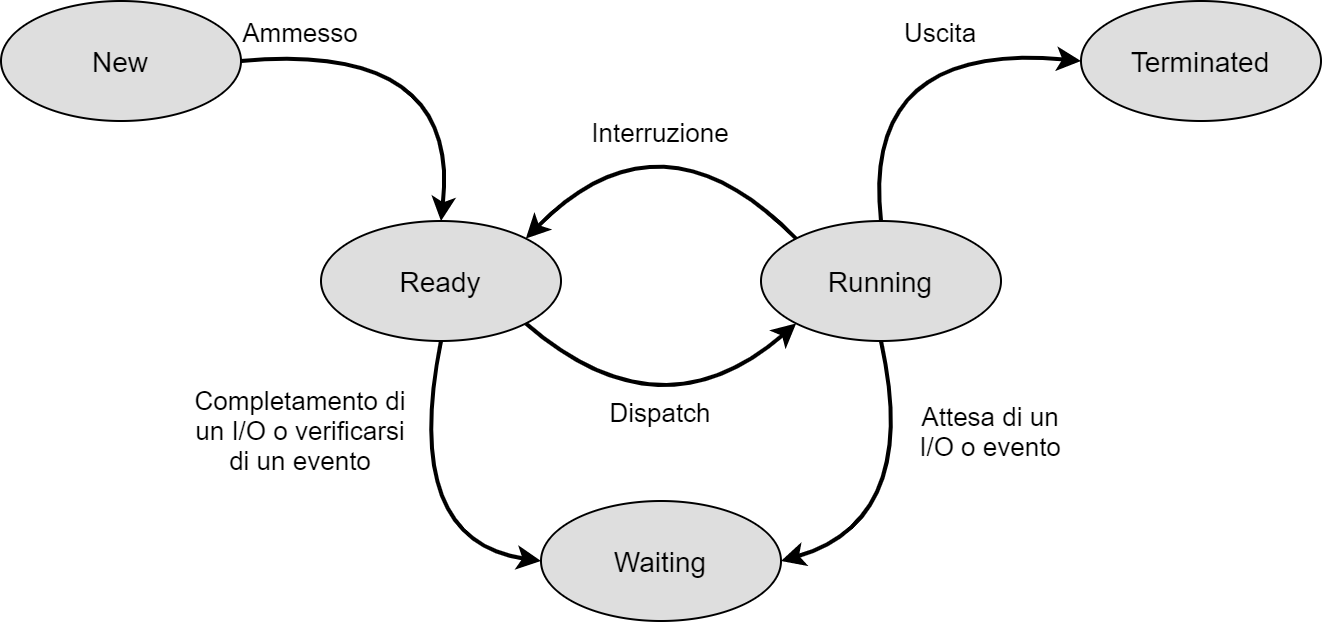
\includegraphics[width=0.9\textwidth]{img/img7.png}
            \caption{Diagramma di transizione degli stati di un processo.}
            \label{fig:img7}
        \end{figure}
        
    \subsection{Blocco di controllo del processo}
        Ogni processo è rappresentato nel sistema operativo da un \textbf{PCB}, \textit{process control block}, il quale contiene molte informazioni connesse a un processo, fra cui le seguenti:
        \begin{itemize}
            \item \textbf{Stato del processo.}
            \item \textbf{Contatore di programma.} Contiene l'indirizzo della seguente istruzione da eseguire per tale processo.
            \item \textbf{Registri della CPU.} Essi variano in numero e tipo in base all'architettura del calcolatore, ma possono includere accumulatori, registri indice, etc.
            \item \textbf{Informazioni sullo scheduling di CPU.}
            \item \textbf{Informazioni sulla gestione della memoria.} Possono includere diverse informazioni in base al sistema di gestione della memoria usato dal sistema operativo, fra cui valore dei registri di base e di limite, tabelle delle pagine o dei segmenti, etc.
            \item \textbf{Informazioni di accounting.} Includono la quota e il tempo di uso della CPU, i limiti di tempo, i numeri dei processi, etc.
            \item \textbf{Informazioni sullo stato dell'I/O.} Lista dei dispositivi assegnati a un dato processo, lista dei file aperti, etc.
        \end{itemize}
        
        In sintesi, il PCB si usa semplicemente come deposito per tutte le informazioni relative ai vari processi.
        
    \subsection{Thread}
        Fino ad ora abbiamo dato per scontato che un processo segue un singolo percorso di esecuzione, una singola sequenza di istruzioni, pur riservandosi il privilegio di metterla in pausa per avviarne temporaneamente un'altra.
        
        Questo paradigma è tuttavia limitante, specialmente nei sistemi multicore, ed infatti viene introdotto il concetto di \textbf{thread}, ossia un percorso di esecuzione che può essere eseguito in parallelo con altri. Le relative informazioni necessarie ai thread vengono aggiunte al PCB.
        
\section{Scheduling dei processi}
    L'obiettivo della multiprogrammazione è quello di tenere sempre almeno un processo attivo, e idealmente tanti quanti ne sono le CPU. Quando un processo va in stato di attesa, lo \textbf{scheduler dei processi} va a selezionarne un altro dalla lista dei processi in attesa. Lo scopo è ovviamente quello di massimizzare l'utilizzo della CPU. Il numero di processi in memoria in un dato istante è detto \textbf{grado di multiprogrammazione}.
    
    È bene considerare inoltre anche la natura dei processi. Parliamo di processi \textbf{I/O bound} nel caso di processi che impiegano la maggior parte del loro tempo in operazioni di lettura e scrittura, mentre parliamo di processi \textbf{CPU bound} nel caso di processi che impiegano la maggior parte del loro tempo in operazioni di elaborazione.
    
    \subsection{Code di scheduling}
        Ogni processo è inserito in una coda di processi pronti chiamata \textit{ready queue}, e sono generalmente implementati come liste concatenate.
        
        Supponiamo che un processo venga assegnato a un core della CPU, ma che in un certo momento esso richieda un input da parte di un disco o tastiera, operazioni generalmente molto lente. Esso, mentre è in attesa di tale input, viene posizionato in una coda d'attesa chiamata \textit{wait queue}.
        
        Un \textbf{nuovo processo} viene inizialmente posizionato nella ready queue fino a che non viene selezionato per essere eseguito (\textit{dispatched}). A questo punto inizia a eseguire le sue elaborazioni e si può verificare uno dei seguenti scenari:
        \begin{itemize}
            \item Il processo può emettere una richiesta di I/O e quindi essere assegnato a una coda di I/O.
            \item Il processo può creare un nuovo processo figlio e attenderne la terminazione.
            \item Il processo può essere rimosso forzatamente dalla CPU a causa di una interruzione ed essere messo nella coda dei processi pronti.
        \end{itemize}
        
        Un processo continua questo ciclo fino al completamento della sua esecuzione: a questo punto viene rimosso da tutte le code e vengono deallocati il suo PCB e le sue risorse.
        
        \begin{figure}[h]
            \centering
            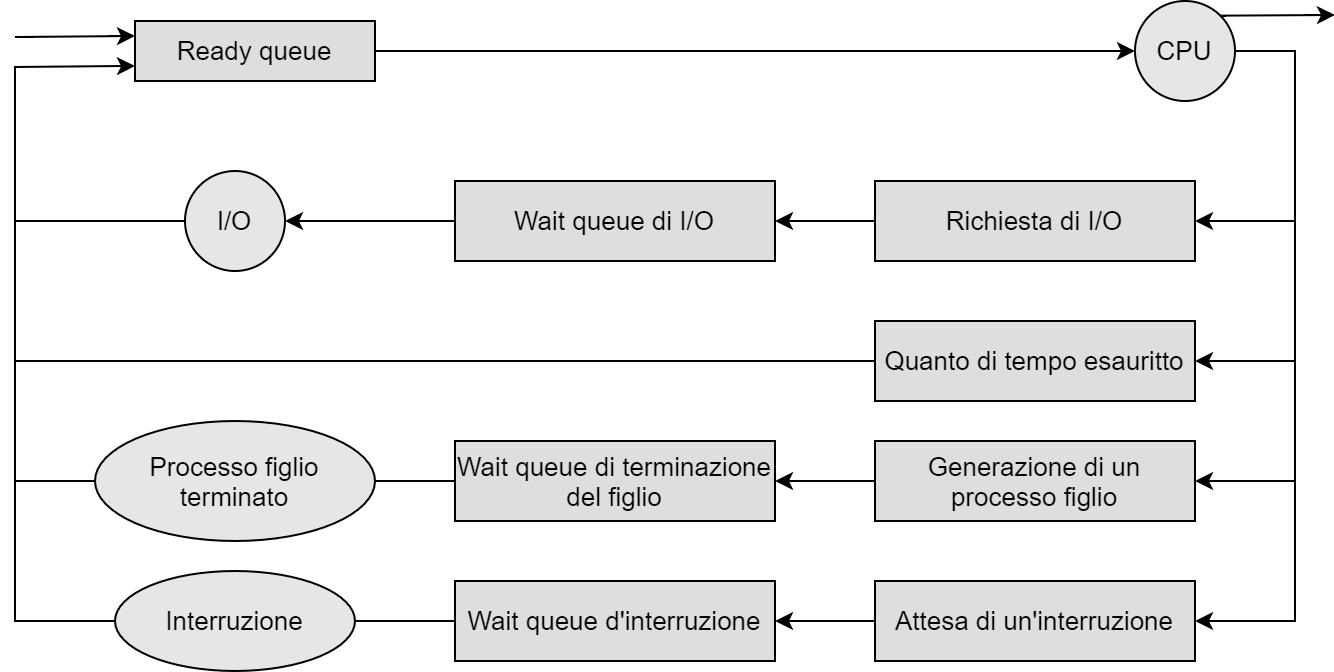
\includegraphics[width=0.95\textwidth]{img/img8.png}
            \caption{Diagramma di accodamento per lo scheduling dei processi.}
            \label{fig:img8}
        \end{figure}
        
    \subsection{Scheduling della CPU}
        Un processo pronto deve essere assegnato a un core della CPU per consentirne l'esecuzione, ed è proprio questo il compito dello scheduler della CPU.
        
        Un processo \textbf{I/O bound} potrà restare in esecuzione per pochi millisecondi prima di tornare in attesa di un input, mentre un processo \textbf{CPU bound} potrà restare in esecuzione per un tempo più lungo. Tuttavia è improbabile che lo scheduler della CPU lasci in esecuzione processi per periodi prolungati. Tenderà invece a rimuovere forzatamente un processo dalla CPU per metterlo in attesa, così da non dare la possibilità a nessun processo di monopolizzare le risorse.
        
        Alcuni sistemi operativi hanno una forma intermedia di scheduling, chiamata \textbf{swapping}. Questa tecnica prevede la rimozione di un processo dalla memoria (\textit{swap-out}) per diminuire il grado di multiprogrammazione e quindi la contesa per la CPU, per poi reintrodurre il processo swappato (\textit{swap-in}) in seguito, nello stato in cui è stato lasciato l'ultima volta. Questo schema è solitamente utilizzato solo quando abbiamo un sovraccarico di memoria.
        
    \subsection{Cambio di contesto}
        Quando un'interruzione forza il sistema a sospendere il lavoro attuale della CPU, c'è necessità di salvare il \textbf{contesto} del processo corrente, per poterlo ripristinare in seguito.
        
        Il contesto è rappresentato all'interno del PCB del processo, e comprende i valori dei registri della CPU, lo stato del processo e informazioni relative alla gestione della memoria. In termini generali parliamo di \textbf{salvataggio dello stato} corrente della CPU e susseguentemente \textbf{ripristino dello stato}.
        
        Il passaggio della CPU a un nuovo processo implica il salvataggio del contesto corrente e il ripristino del contesto del nuovo processo. Questa procedura è chiamata \textbf{cambio di contesto}, o \textit{context switch}. Il context switch è puro overhead, siccome il sistema esegue operazioni atte alla gestione dei processi senza nessun tipo di computazione.

\section{Operazioni sui processi}
    Il sistema operativo deve fornire metodi per creare e cancellare i processi, i quali devono poter essere cariati e rimossi dinamicamente.
    
    \subsection{Creazione di processi}
        Un processo può creare altri processi. Il processo che crea viene chiamato processo \textbf{genitore}, o \textbf{padre}, mentre il processo creato viene chiamato processo \textbf{figlio}. Questo processi possono creare altri processi, creando così un \textbf{albero} di processi.
        
        La maggior parte dei sistemi operativi identifica un processo per mezzo di un numero unico, solitamente un intero, chiamato \textbf{identificatore del processo} o \textbf{pid} (\textit{process identifier}). Questo è utile per identificare univocamente i processi e gestirli.
        
        In Linux (dove generalmente si preferisce il termine \textit{task} ma qui usiamo processo in maniera generica), abbiamo per esempio \texttt{systemd} che è il processo padre di tutti i processi utente e ha sempre \texttt{pid} uguale a 1.
        
        Solitamente un processo figlio avrà bisogno di determinante risorse, fra cui dispositivi di I/O, memoria, etc. Può ottenere queste risorse direttamente dal sistema operativo oppure ereditarle dal processo padre. Quando un processo va a creare figli può spartire le proprie risorse o una sottoinsieme di esse fra i figli. Questa cosa ha fra l'altro lo scopo di non sovraccaricare troppo il sistema, cosa che potrebbe succedere se un processo iniziasse a creare figli affamati di risorse in maniera incontrollata. Oltre a risorse il processo padre può passare ai figli anche dei parametri di inizializzazione.
        
        Quando un processo ne crea uno nuovo, ci sono due possibilità per quanto riguarda l'esecuzione:
        \begin{enumerate}
            \item Il processo genitore continua la sua esecuzione in maniera concorrente con i propri figli.
            \item Il processo genitore attente che alcuni o tutti i suoi figli terminino.
        \end{enumerate}
        
        Ci sono allo stesso modo due possibilità per quanto riguarda lo spazio di indirizzi del nuovo processo:
        \begin{enumerate}
            \item Il processo figlio è un duplicato del processo genitore (ha stessi programma e dati).
            \item Nel processo figlio si carica un nuovo programma.
        \end{enumerate}
        
    \subsection{Terminazione di un processo}
        Un processo termina quando finisce l'esecuzione della sua ultima istruzione e inoltra la richiesta al sistema operativo di essere cancellato. Il processo può riportare un'informazione di stato al processo padre, e tutte le risorse occupate, comprese memoria fisica e virtuale, file e dispositivi di I/O vengono liberati dal sistema operativo.
        
        Un processo può anche terminare prematuramente, e questa operazione è eseguita dal genitore. Il motivo è di sicurezza, in quanto se così non fosse un utente potrebbe arbitrariamente provocare la terminazione di qualsiasi processo. Un genitore deve, quindi, conoscere le identità dei propri figli per terminarli, ed è per questo che quando un processo viene creato, la propria identità viene passata al processo genitore.
        
        Un processo genitore può porre termine all'esecuzione di uno dei suoi processi figli per vari motivi, fra quali i seguenti:
        \begin{itemize}
            \item Il processo figlio ha ecceduto nell'utilizzo di alcune risorse che gli sono state concessi. Ciò richiede che il processo padre disponga di informazioni circa lo stato dei propri figli.
            \item Il compito assegnato al processo figlio non è più richiesto.
            \item Il processo genitore termina e il sistema operativo non consente l'esistenza di tali situazioni.
        \end{itemize}
        
        In alcuni sistemi operativi, se un processo termina, terminano anche tutti i suoi figli, a prescindere dalla natura della terminazione (normale o anormale). In questo caso si parla di \textbf{terminazione a cascata}.
        
        Quando un processo termina le sue risorse vengono deallocate dal sistema operativo. Tuttavia, la sua voce nella tabella dei processi deve rimanere fino a quando il padre chiama \texttt{wait()}, perché la tabella dei processi contiene lo stato di uscita del processo.
        
        Un processo che è terminato, ma il cui genitore non ha ancora chiamato la \texttt{wait()}, è detto processo \textbf{zombie}. Tutti i processi entrano in questo stato dopo la loro terminazione, ma solitamente ci restano solo per breve tempo. Una volta che il loro genitore chiama la \texttt{wait()}, il \textit{pid} del processo zombie e la sua voce nella tabella dei processi vengono rilasciati.
        
        Consideriamo ora un genitore che termina senza invocare la \texttt{wait()}. Esso lascia i processi figli come orfani. Alcuni sistemi operativi, come Linux e UNIX, affrontano questa situazione facendo diventare il processo radice (\texttt{init} per UNIX e \texttt{systemd} per Linux) il nuovo genitore dei processi orfani. Inoltre il processo radice chiama periodicamente la \texttt{wait()} per liberare le risorse.
        
    \subsection{Comunicazione tra processi}
        Processi eseguiti concorrentemente nel sistema operativo possono essere \textit{indipendenti}, nel caso in cui non influiscano o subiscano l'influenza di altri processi durante la loro esecuzione, o \textit{cooperanti} nel caso contrario. Ovviamente l'essere o meno indipendente è fortemente collegato alla condivisione di dati fra processi.
        
        Alcuni motivi dell'utilità di un ambiente che consente la cooperazione fra processi:
        \begin{itemize}
            \item \textbf{Condivisione d'informazioni:} In questo modo più utenti possono accedere concorrentemente a risorse a cui sono interessate, come un file condiviso.
            
            \item \textbf{Velocizzazione del calcolo:} Se l'elaboratore dispone di più core di elaborazione, alcune attività possono essere suddivide in sottoattività eseguibili in parallelo, causando un aumento delle prestazioni.
            
            \item \textbf{Modularità:} Può essere utile la costruzione di un sistema modulare, che consente la suddivisione di funzioni di sistema in processi o thread.
        \end{itemize}
        
        Necessitiamo quindi di un meccanismo di comunicazione fra processi (\textbf{IPC}, \textit{interprocess comunication}). I due modelli principali sono quello a \textbf{memoria condivisa}, in cui si stabilisce una zona di memoria condivisa dai processi cooperanti, che possono leggere e scrivere da tale zona, e quello a \textbf{scambio di messaggi}.
        
        Io modello a memoria condivisa è più rapido, ma potrebbe creare problemi di sincronizzazione e accesso concorrente, mentre quello a scambio di messaggi è più facile da implementare, meno prono agli errori ma anche meno efficiente, e infatti è usato per scambiare piccole moli di dati. Nei sistemi operativi moderni troviamo entrambi i modelli, spesso nello stesso sistema.

\chapter{Parte Seconda, Capitolo 4: Thread e Concorrenza}
\section{Introduzione}
    Fino ad ora abbiamo considerato i processi come aventi un unico processo di controllo. Tuttavia questo non è vero nella maggior parte dei sistemi operativi moderi, in quanto essi dispongono di più processi di controllo all'interno dello stesso processo chiamati \textbf{thread}. Con l'aumentare dei core è importante identificare opportunità di parallelismo per aumentare, talvolta drasticamente, le performance del sistema.
    
    Un \textbf{thread} è l'unità di base d'uso della CPU e comprende un identificatore di thread (ID), un contatore di programma, un insieme di registri e una pila (\textit{stack}). Condivide con gli altri thread che appartengono allo stesso processo al sezione del codice, la sezione dei dati e altre risorse di sistema come file aperti e segnali. Un processo tradizionale, chiamato anche \textbf{processo pesante} (\textit{heavyweight process}), è composto da un solo thread. Un processo multithread è capace di svolgere più compiti in maniera concorrente.
    
    \begin{figure}[h]
        \centering
        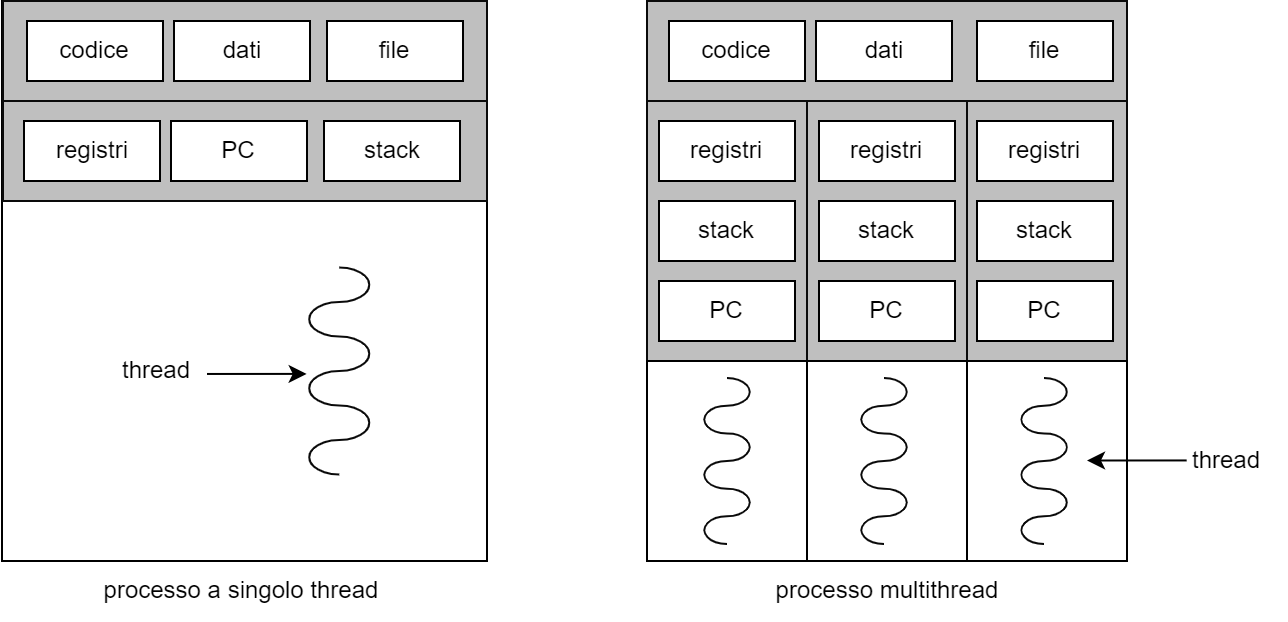
\includegraphics[width=1\textwidth]{img/threads.png}
        \caption{Differenza fra processo a singolo thread e multithread}
        \label{fig:my_label}
    \end{figure}
    
    \subsection{Motivazioni}
        La maggior parte delle applicazioni per computer moderni è \textbf{multithread}. Di solito si codifica come un processo a sé stante comprendente più thread di controllo. Per esempio possiamo avere un'applicazione galleria che usa diversi thread per creare diverse thumbnail, o un browser web che usa thread per rappresentare immagini e testo e uno per scaricare dati dalla rete.
        
        Possiamo pensare, prendendo per esempio un server web utilizzato da moltissimi utenti contemporaneamente, la creazione di un processo che a ogni richiesta utente crea un altro processo che soddisfa la richiesta, per esempio la restituzione di una pagina web. Questa tecnica è stata effettivamente usata per molto tempo, ma questo è un caso in cui molti processi devono eseguire compiti simili fra loro. Creare un processo è dispendioso, e quanto più i compiti che devono eseguire sono simili, tanto meno vale la pena di creare nuovi processi per ogni compito. L'evoluzione naturale di ciò è creare un processo multithread che crea appunto \textbf{thread} per le varie richieste che riceve.
        
        La maggior parte dei kernel è multithread. Durante l'avvio di Linux per esempio sono creati diversi thread e ognuno si occupa di una diversa fase dell'inizializzazione del sistema. Possiamo notare che in Linux abbiamo il thread \texttt{kthreadd} (pid = 2) che funge da genitore di tutti gli altri thread a livello kernel.
        
        Molti algoritmi, come quelli di ordinamento e gli algoritmi per alberi e grafi, possono trovare grandi vantaggi dal multithreading. Ovviamente queste non sono le uniche applicazioni, e anche in ambito di data mining, intelligenza artificiale, grafica etc. possono essere e sono usate tecniche per avvalersi della potenza dei moderni sistemi multicore.
        
    \subsection{Vantaggi}
        I vantaggi della programmazione multithread si possono classificare in quattro categoria principali.
        \begin{enumerate}
            \item \textbf{Tempo di risposta.} Rendere multithread un'applicazione interattiva potrebbe, in casi moderni, essere l'unico modo di garantire una buona esperienza utente, in quanto il sistema può elaborare l'input utente e continuare la sua esecuzione. Si consideri un'interfaccia utente, e in particolare l'utilizzo di un mouse. In un'applicazione a thread singolo il sistema potrebbe gestire il cursore o eseguire funzioni, mentre in un sistema multithread queste cose si possono separare.
            
            \item \textbf{Condivisione delle risorse.} Un processo deve specificare se vuole condividere risorse tramite l'utilizzo di memoria condivisa o scambio di messaggi, mentre i thread dispongono di memoria condivisa di default. Dunque un'applicazione può avere thread che eseguono attività diverse ma hanno accesso allo stesso codice e dati, e tutti nello stesso spazio di indirizzi.
            
            \item \textbf{Economia.} Assegnare memoria e risorse per un nuovo processo può essere costoso, tanto che conviene spesso creare nuovi thread e gestirne il context switch, in quanto essi condividono le stesse risorse e rendono non necessaria una nuova inizializzazione.
            
            \item \textbf{Scalabilità.} Il multithreading su una macchina multicore incrementa il parallelismo. Nel caso di un programma a thread singolo, potremmo sfruttare comunque un solo core per volta, lasciando buona parte delle capacità di computazione del sistema non usate.
        \end{enumerate}
        
\section{Programmazione multicore}
    Nel corso della storia, in risposta a una richiesta di maggiore capacità di calcolo si è passati da sistemi con una singola CPU a sistemi con più CPU, e in seguito a sistemi con più \textit{core} per singolo chip, i quali vengono visti dal sistema operativo come processori separati. Un tipo di programmazione multithread sfrutta molto meglio questo tipo di architettura.
    
    Si noti la differenza fra \textbf{parallelismo} e \textbf{concorrenza}. Un sistema concorrente supporta più task permettendo a ciascuno di progredire nell'esecuzione. Un sistema parallelo invece può eseguire contemporaneamente più task.
    
    \subsection{Tipi di parallelismo}
        In generale, esistono due tipi di parallelismo: parallelismo dei dati e parallelismo delle attività.
        
        Il \textbf{parallelismo dei dati} prevede la suddivisione di una certa mole di dati su più core e l'esecuzione delle stesse operazioni su ogni sottoinsieme dei dati.
        
        Il \textbf{parallelismo delle attività} prevede la distribuzione di attività (thread) su più core, e non di dati. Ogni thread realizza un'operazione distinta, e più thread possono operare sugli stessi dati o su dati diversi.
        
        Questi due tipi di parallelismo non sono mutualmente esclusivi, e le applicazioni possono utilizzare un ibrido di queste due strategie.
        
    \section{Modelli di supporto al multithreading}
        I thread possono essere distinti in \textbf{thread a livello utente} e \textbf{thread a livello kernel}: i primi sono gestiti sopra al livello kernel e senza il suo supporto; i secondi sono gestiti direttamente dal sistema operativo.
        
        In ogni caso deve esistere una relazione fra questi due livelli. Ne analizziamo tre opzioni.
        \begin{figure}[h]
                \centering
                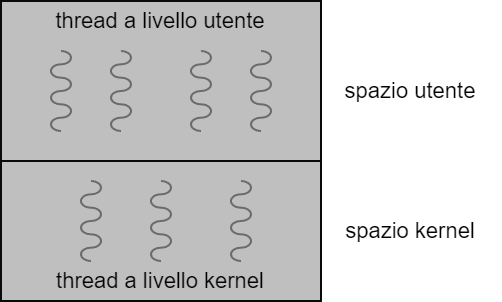
\includegraphics[width=0.5\textwidth]{img/thread1.png}
                \caption{Thread a livello utente e a livello kernel}
                \label{fig:thread1}
            \end{figure}
        
        \subsection{Modello da molti a uno}
            In questo modello, molti thread a livello utente corrispondono a un solo thread a livello kernel. La gestione dei thread risulta efficiente, ma tutto il processo rimane bloccato nel caso in cui un thread invochi una chiamata di sistema di tipo bloccante. Inoltre, poiché un solo thread alla volta può accedere al kernel, è impossibile eseguire thread multipli in sistemi multicore: ne deriva che questo modello è poco utilizzato nei sistemi moderni.
            
            \begin{figure}[h]
                \centering
                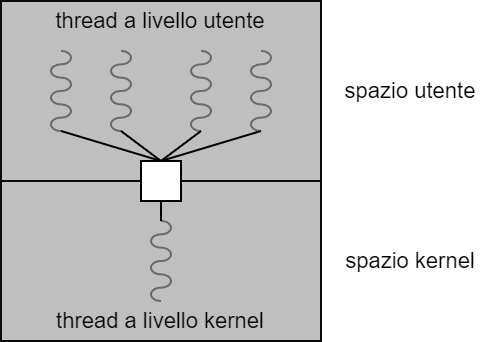
\includegraphics[width=0.5\textwidth]{img/thread2.png}
                \caption{Modello da molti a uno}
                \label{fig:my_label}
            \end{figure}
            
            
        \subsection{Modello da uno a uno}
            Questo modello mette in corrispondenza ciascun thread a livello utente con un thread a livello kernel. Questo modello offre un maggior grado di concorrenza, in quanto anche se un thread effettua una chiamata bloccante è comunque possibile eseguire un altro thread, e inoltre consente anche l'esecuzione parallela di thread in sistemi multiprocessore. Lo svantaggio di questo modello è che per ogni thread a livello utente va creato un thread a livello kernel, e ciò può creare problemi di prestazioni. Infatti nonostante questo modello sia utilizzato su sistemi della famiglia Windows e Linux, c'è un limite al numero di thread che è possibile creare.
            
            \begin{figure}[h]
                \centering
                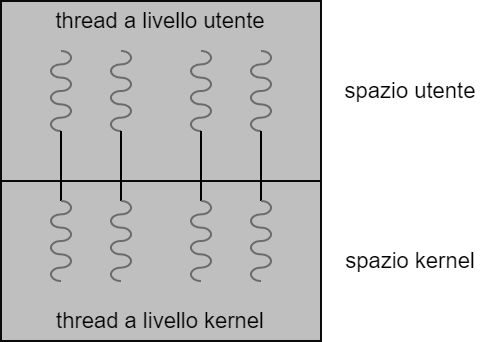
\includegraphics[width=0.5\textwidth]{img/thread3.png}
                \caption{Modello da uno a uno}
                \label{fig:my_label}
            \end{figure}
            
        \subsection{Modello da molti a molti}
            Questo modello mette in corrispondenza un certo numero di thread a livello utente con un numero minore o uguale di thread a livello kernel. Questo numero può variare in base all'applicazione o al calcolatore. Possiamo per esempio assegnare più thread in un'architettura dotata di otto core rispetto a quanti ne verrebbero assegnati in un'architettura dotata di quattro core.
            
            Per quanto riguarda la concorrenza, abbiamo visto che il modello molti a uno non la supporta in quanto possiamo scegliere un solo thread utente alla volta, mentre quello uno a uno la supporta, ma con la clausola di non creare troppi thread. Il modello molti a molti non ha nessuno di questi problemi, in quanto il programmatore può creare tutti i thread che ritiene necessario ed essi possono essere assegnati a diversi thread a livello kernel per l'esecuzione in parallelo. Inoltre una chiamata di sistema bloccante non è un grande problema, in quanto in questo caso il kernel può schedulare un altro thread.
            
            Una variante di questo modello prevede comunque la corrispondenza fra un certo numero di thread utente e un numero minore o uguale di thread kernel, ma permette anche di vincolare un singolo thread utente a un thread kernel. Questa variante è chiamata \textbf{modello a due livelli}.
            
            Nonostante il modello molti a molti sembri il più flessibile, è difficile metterlo in pratica. Inoltre, il limite di thread a livello kernel si alza con l'aumentare dei core di elaborazione, e diventa sempre meno importante.
            
            \begin{figure}[h]
                \centering
                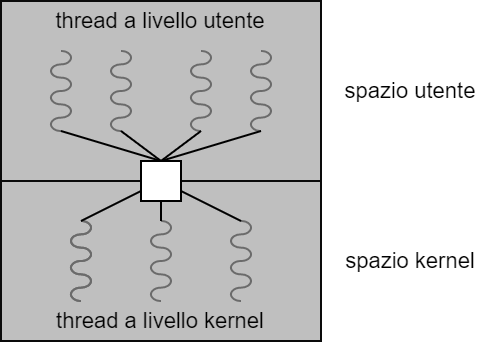
\includegraphics[width=0.7\textwidth]{img/thread4.png}
                \caption{Modello da molti a molti}
                \label{fig:my_label}
            \end{figure}
            
            \newpage
            \begin{figure}
                \centering
                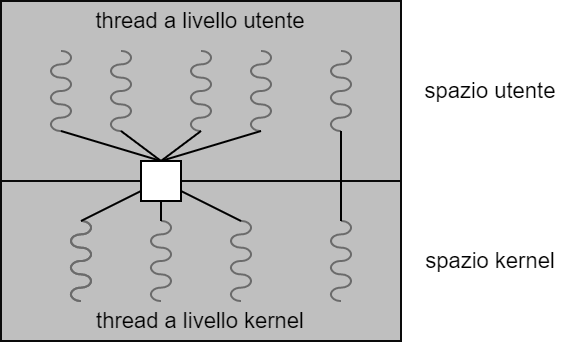
\includegraphics[width=0.7\textwidth]{img/thread5.png}
                \caption{Modello a due livelli}
                \label{fig:my_label}
                \vspace{5.6in}
            \end{figure}

\chapter{Parte Seconda, Capitolo 5: Scheduling della CPU}
In un sistema operativo abbiamo bisogno di schedulare i processi per aumentare l'efficienza; sia esso single o multi core, eseguire i processi in maniera sequenziale non sfrutta i molti istanti in cui quel processo attende input, output o eventi, lasciando a tutti gli effetti il sistema in \textit{idle}.

\section{Concetti fondamentali}
    Come detto prima, lo scopo di un calcolatore è quello di minimizzare il tempo di idle, quindi è conveniente schedulare i processi in maniera che i tempi di attesa di uno vengano riempiti da tempi di elaborazione di un altro. Ogni risorsa di un elaboratore viene sottoposta a scheduling, e ovviamente la CPU è una delle risorse principali.
    
    \subsection{Ciclicità delle fasi di elaborazione e di I/O}
        Un concetto importante e che potrebbe guidare la scelta di un adeguato algoritmo di scheduling della CPU è capire come i processi alternano due fasi: una fase di \textbf{elaborazione}, in cui il lavoro è a carico della CPU, e la fase di \textbf{I/O}, in cui sono invece i vari dispositivi di input e output a fare il grosso del lavoro.
        
        È naturale pensare che i processi si comportino così: un processo ottiene dei dati (I/O) che procede a elaborare (CPU), per poi comunicare al sistema o a un altro processo il risultato di questa elaborazione (I/O) e ricominciare così il ciclo.
        
        Chiamiamo queste fasi del ciclo \textit{I/O burst} e \textit{CPU burst}, e indubbiamente alcuni tipi di processi possono avere un bilanciamento di queste due fasi diverso, e ciò può certamente influenzare la scelta o la progettazione di un algoritmo di scheduling.
        
    \subsection{Scheduler della CPU}
        Quando la CPU incontra un momento di inattività, viene scelto un elemento dalla \textit{ready queue} per essere eseguito in modo da non lasciare il sistema in uno stato di idle.
        
        Questa scelta viene fatta dallo \textbf{scheduler a breve termine}, o \textbf{scheduler della CPU}. La ready queue non è necessariamente una coda FIFO, ma potrebbe essere una qualsiasi struttura: coda FIFO, a priorità, albero, lista concatenata non ordinata, eccetera.
        
        Concettualmente, tutti i processi della ready queue sono posti in lista d'attesa per accedere alla CPU. Generalmente gli elementi delle code sono i PCB dei processi.
        
    \subsection{Scheduling con e senza prelazione}
        Le decisioni riguardanti lo scheduling della CPU vengono prese nelle seguenti quattro circostanze:
        \begin{enumerate}
            \item Un processo passa dallo stato di esecuzione allo stato di \textit{wait}.
            \item Un processo passa dallo stato di esecuzione allo stato di \textit{ready}.
            \item Un processo passa dallo stato di attesa allo stato di \textit{ready}.
            \item Un processo viene terminato.
        \end{enumerate}
        
        I casi 1 e 4 non danno alternative in termini di scheduling: si deve scegliere un nuovo processo dalla ready queue. Una scelta invece si può fare nei casi 2 e 3.
        
        Quando lo scheduling interviene solo nelle condizioni 1 e 4, si dice \textbf{senza prelazione} (\textit{nonpreemptive}) o \textbf{cooperativo} (\textit{cooperative}). Altrimenti, lo schema di scheduling è \textbf{con prelazione} (\textit{preemptive}).
        
        Nel caso dello scheduling senza prelazione, quando si assegna la CPU a un processo, questo ne rimane in possesso fino al suo rilascio, dato dalla terminazione o dal suo passaggio allo stato di attesa. Praticamente tutti i sistemi operativi moderni usano invece lo scheduling con prelazione.
        
        Un lato negativo dello scheduling con prelazione è che può portare a \textit{race condition} nel caso di dati condivisi fra i processi, si consideri per esempio il caso in cui un processo venga messo in wait e un secondo processo tenti di accedere a dati lasciati dal processo precedente in uno stato incoerente.
        
    \subsection{Dispatcher}
        Questo è un altro elemento coinvolto nelal funzione di scheduling, ed in particolare passa effettivamente il controllo della CPU al processo scelto dallo scheduler. Questa funzione comprende:
        \begin{itemize}
            \item Il context switch da un processo a un altro;
            \item Il passaggio alla modalità utente;
            \item Il salto alla giusta posizione del programma utente per riavviarne l'esecuzione.
        \end{itemize}
        
        Poiché si attiva a ogni cambio di contesto, il \textbf{dispatcher} dovrebbe essere più veloce possibile. Il tempo necessario per fermare un processo ed avviare l'esecuzione di un altro è noto come \textbf{latenza di dispatch}.
        
        Un'altra distinzione che possiamo fare è quella fra cambi di contesto volontari e non volontari. Un cambio di contesto \textbf{volontario} avviene quando un processo cede il controllo della CPU dopo aver richiesto una risorsa al momento non disponibile, per esempio quando è bloccato in una richiesta I/O. Un cambio di contesto \textbf{non volontario} si verifica quando la CPU viene sottratta a un processo, per esempio quando il suo tempo è scaduto o quando è stata eseguita la prelazione a favore di un processo a priorità più alta.
        
\section{Criteri di scheduling}
    I diversi algoritmi di scheduling possono favorire un certo comportamento o una certa classe di processi. Per il confronto fra algoritmi ci sono una serie di criteri da prendere in considerazione, fra cui:
    \begin{itemize}
        \item \textbf{Utilizzo della CPU:} La CPU deve essere più attiva possibile. In teoria può andare dallo 0 al 100 per cento. In un sistema reale dovrebbe dal 40 per cento al 90 per cento.
        
        \item \textbf{Throughput:} La CPU è attiva quando si svolge del lavoro. Una misura del lavoro può essere data dalla quantità di processi completati nell'unità di tempo. Tale misura è detta \textbf{produttività}, o \textit{throughput}. Per processi di lunga durata il suo valore può essere anche di un processo all'ora, mentre per processi di breve durata anche di 10 processi al secondo.
        
        \item \textbf{Tempo di completamento:} Il criterio più importante dal punto di vista del processo stesso è il tempo di completamento dello stesso. L'intervallo che intercorre tra la sottomissione del processo e il completamento dell'esecuzione è detto \textbf{tempo di completamento} o \textit{turnaround time}, ed è la somma dei tempi passati nell'attesa dell'ingresso in memoria, nella ready queue, durante l'esecuzione della CPU e nelle operazioni di I/O.
        
        \item \textbf{Tempo di attesa.} L'algoritmo di scheduling non influisce sul tempo necessario per completare un processo, ma solo sul tempo che lo stesso passa in attesa nella ready queue. Il \textbf{tempo d'attesa} è la somma di tutte queste attese.
        
        \item \textbf{Tempo di risposta.} In un sistema interattivo il tempo di completamento non può essere il miglior criterio di valutazione. Una misura di confronto più adatta è il tempo che intercorre fra una richiesta e la relativa risposta prodotta, ed è chiamata \textbf{tempo di risposta}, ed è data dal tempo necessario per iniziare la risposta ma non dal tempo necessario per completare l'output.
    \end{itemize}
    
    È auspicabile massimizzare l'utilizzo e la produttività della CPU e minimizzare il tempo di completamento, attesa e risposta. Spesso si punta a ottimizzare i valori medi, ma in alcuni casi si potrebbe puntare a ottimizzare quelli medi o massimi, per esempio per assicurare che tutti gli utenti ottengano un buon servizio potremmo voler ridurre il massimo tempo di risposta.
    
\section{Algoritmi di scheduling}
    Lo scheduling della CPU si occupa di decidere quale dei processi della ready queue andrà assegnato al core della CPU. Ci sono diversi algoritmi per ottenere ciò in maniera efficiente. Nonostante la maggior parte dei sistemi moderni dispongano di core multipli, andremo a vederne qualcuno nel contesto di una singola CPU con un singolo core disponibile.
    
    \subsection{Scheduling in ordine d'arrivo}
        Il più semplice algoritmo di scheduling è lo \textbf{scheduling in ordine d'arrivo} (\textit{scheduling first-come, first-served}, o FCFS). Con questo schema la CPU si assegna sul processo che la richiede per primo, e si basa su una semplice coda FIFO.
        
        Il problema con questo algoritmo è che il tempo medio d'attesa è piuttosto alto. Si considerino i seguenti processi con la durata delle operazioni espressa in millisecondi:
        
        \begin{table*}[h]
            \centering
            \begin{tabular}{c c}
                \textbf{Processo} & \textbf{Durata della sequenza} \\ \hline
                $P_1$ & 24\\
                $P_2$ & 3\\
                $P_3$ & 3\\
                \hline
            \end{tabular}
            \label{tab:my_label}
        \end{table*}
        
        Eseguendo i processi in ordine abbiamo un tempo di attesa di $0$ per $P_1$, di $24$ per $P_2$ e di $27$ per $P_3$, e quindi un tempo di attesa medio di 17 millisecondi. Se i processi arrivassero in ordine $P_2, P_3, P_1$, il tempo di attesa medio sarebbe di appena 3 millisecondi.
        
        Un modello del genere potrebbe anche causare un \textbf{effetto convoglio}, in cui molti processi dal breve tempo di elaborazione attendono che un processo pesante termini, il che può causare un utilizzo diminuito sia della CPU che dei dispositivi.
        
        Inoltre questo algoritmo è senza prelazione, e abbiamo visto precedentemente perché ciò non è ideale. In casi estremi un singolo processo estremamente pesante potrebbe occupare la CPU per un tempo lunghissimo, privando il resto del sistema delle risorse.
        
    \subsection{Scheduling shortest-job-first}
        Un criterio di scheduling diverso è lo \textbf{scheduling per brevità} (\textbf{shortest-job-first}, o \textit{SJF}), che determina per ogni processo la lunghezza del prossimo CPU burst ed esegue quello con il valore più piccolo al fine di diminuire il tempo di attesa medio. Come detto, non viene davvero presa in considerazione la lunghezza dell'intero job ma solo del prossimo CPU burst, e infatti il nome è traviante ma è comunemente usato.
        
        Si può dimostrare che l'algoritmo SJF è \textit{ottimale}, ossia minimizza il tempo di attesa medio. Nonostante ciò, non è realizzabile in pratica in quanto non si può conoscere in anticipo la durata di un CPU burst. Possiamo come alternativa cercare di predirla in base a euristiche, come per esempio il fatto che per una stessa operazione le durate dei suoi CPU burst saranno simili.
        
        La lunghezza del prossimo CPU burst si definisce solitamente usando la \textbf{media esponenziale} delle lunghezze misurate dei precedenti CPU burst. Essa si calcola con la seguente formula: siano $t_n$ la lunghezza dell'$n$-esimo CPU burst della CPU e $\tau_{n+1}$ il valore previsto per il successivo burst. Allora, dato $\alpha \colon 0 \leq \alpha \leq 1$, si definisce
        \begin{equation*}
            \tau_{n+1} = \alpha t_n + (1 - \alpha)\tau_n
        \end{equation*}
        Il valore $t_n$ contiene le informazioni più recenti; $\tau_n$ registra la storia passata. Il parametro $\alpha$ controlla il peso relativo sulla predizione della storia decente e di quella passata. Il $\tau_0$ iniziale si può definire come un valore assoluto o una media di sistema.
        
        L'algoritmo SJF può essere sia con prelazione che senza prelazione. La scelta si presenta nel momento in cui un processo richiede la CPU mentre un altro processo è ancora in esecuzione. Il nuovo processo potrebbe richiedere un CPU burst più breve di quello rimanente al processo in esecuzione, e un algoritmo SJF con prelazione sostituisce il processo attualmente in esecuzione. Lo schema SJF con prelazione è talvolta chiamato \textit{shortest-remaining-time-first}.
        
    \subsection{Scheduling circolare (\textit{round-robin})}
        L'\textbf{algoritmo di scheduling circolare} (\textit{round-robin}, RR) è simile allo scheduling FCFS, ma aggiunge la capacità di prelazione in modo che il sistema possa commutare fra i vari processi. Viene fissato un \textbf{quanto} o \textbf{porzione} di tempo, che di solito è compreso fra i 10 e i 100 millisecondi, e la ready queue viene trattata come una coda circolare. Lo scheduler scorre la ready queue e assegna a ogni processo al massimo un quanto di tempo.
        
        La ready queue è implementata come una coda FIFO e si comporta in questo modo: i nuovi processi vengono aggiunti alla fine della coda, mentre un processo in esecuzione può avere due destini: o conclude la sua esecuzione prima dello scadere del quanto di tempo, le risorse vengono rilasciate e lo scheduler passa al processo successivo della coda, oppure non riesce a terminare la sua esecuzione, viene messo alla fine della ready queue e viene dato un quanto di tempo al processo successivo.
        
        Il tempo di attesa medio per questo algoritmo di scheduling è abbastanza alto.
        
        Le prestazioni di questo algoritmo dipendono dalla dimensione del quanto di tempo. Nel caso limite di un quanto di tempo molto lungo, l'algoritmo si riduce al caso di un FCFS. Nel caso invece di un quanto di tempo molto breve, la maggior parte delle risorse potrebbero essere impiegate per eseguire i context switch. Ecco perché di solito si sceglie un quanto di tempo ampio rispetto alla durata di un context switch.
        
        Anche il \textbf{tempo di completamento} (\textit{turnaround time}) è influenzato dalla dimensione del quanto di tempo.
        
        Il problema in questo caso è quindi stabilire un quanto di tempo adeguato, in quanto esso non deve essere troppo piccolo né troppo grande.
        
    \subsection{Scheduling con priorità}
        L'algoritmo SJF è un caso particolare dell'algoritmo di scheduling con priorità, in cui si assegna a ogni processo una priorità, e nel caso di priorità uguale si usa un criterio FCFS.
        
        Non c'è un consenso sull'utilizzo di numeri bassi per indicare priorità basse o alte, e questo può generare confusione.
        
        Le priorità si possono definire sia \textit{internamente} che \textit{esternamente}. Nel primo caso il criterio è basato su quantità misurabili dal sistema operativo, come stima del tempo per la prossima CPU burst, risorse utilizzate, requisiti di memoria, etc. Le priorità definite esternamente si avvalgono di parametri esterni al sistema operativo, come l'importanza del processo, l'utente che lo richiede, e altri fattori spesso di ordine politico.
        
        Questo algoritmo può essere sia con che senza prelazione. Nel caso di un'implementazione con prelazione, semplicemente all'arrivo di un nuovo processo la sua priorità viene confrontata con quella del processo attualmente in esecuzione ed eventualmente viene eseguita una sostituzione.
        
        Un problema legato a questo algoritmo può essere l'\textbf{attesa indefinita} (\textit{starvation}). Un processo a priorità bassa potrebbe ritrovarsi in attesa indefinita della CPU, costantemente surclassato da processi a priorità alta. Solitamente i due destini di un tale processo sono o di essere eseguito molto tempo dopo la sua richiesta, o di essere perduto in seguito a un eventuale crash del sistema.
        
        Una possibile soluzione sta nell'\textbf{invecchiamento} (\textit{aging}); si tratta di una tecnica che semplicemente aumenta la priorità di un processo man mano che esso invecchia.
        
        Un'altra opzione sta nel combinare round-robin e scheduling a priorità in maniera tale che il sistema esegua i processi allo stesso livello di priorità con un metodo round-robin.
        
    \subsection{Scheduling a code multilivello}
        Negli algoritmi di scheduling visti precedentemente, c'è necessità di cercare il processo con priorità più alta all'interno di una coda, o di ordinare i processi. Questo può essere costoso e spesso, nella pratica, è più utile disporre di diverse code, una per priorità, e lasciare che lo scheduling si occupi di prelevare processi dalla prima coda non vuota a priorità più alta.
        
        Questo processo, noto come \textbf{scheduling a code multilivello}, funziona bene anche quando lo scheduling a priorità è combinato con quello RR. Nella forma generale di questo approccio viene assegnata priorità statica a ciascun processo, il quale rimane nella stessa coda durante tutto il suo tempo di esecuzione.
        
        Possiamo anche definire le code in base a categorie più complesse della semplice priorità. Possiamo per esempio definire una coda per i processi in tempo reale, una per quelli di sistema, una per quelli batch etc. Queste code oltre ad essere collegate fra loro da valori di priorità, possono anche implementare diversi algoritmi di scheduling, in base alla natura dei processi che contengono. Queste code possono avere priorità assoluta fra loro, con o senza prelazione, o possiamo assegnare a ognuna un quanto di tempo diverso per eseguire i suoi processi. È dunque un meta-sistema di organizzazione molto flessibile, che può contenere al suo interno contemporaneamente più modelli e più algoritmi di scheduling.
        
    \subsection{Scheduling a code multilivello con retroazione}
        Nell'algoritmo visto precedentemente, i processi non avevano la possibilità di cambiare coda. Un processo inserito in una coda batch sarebbe rimasto per sempre in quella coda. Questo metodo è rigido ma ha il vantaggio di avere un basso carico di scheduling.
        
        Lo \textbf{scheduling a code multilivello con retroazione} (\textit{multilevel feedback queue scheduling}), invece, permette ai processi di spostarsi fra le code. L'idea sta nel separare i processi in base alle caratteristiche dei loro CPU burst. Se un processo usa la CPU per troppo tempo, viene spostato in una coda a priorità più bassa. In questo modo i processi con prevalenza di I/O e quelli interattivi avranno priorità più alta. Inoltre si può applicare un metodo di \textit{aging} per far passare in code con priorità più alta i processi che hanno aspettato troppo in code con priorità bassa.
        
        Solitamente uno scheduler di questo tipo è caratterizzato da: numero di code, algoritmo di scheduling per ciascuna coda, metodo usato per determinare quando spostare un processo in una coda a priorità maggiore o minore e metodo usato per determinare in quale coda si deve mettere un processo quando richiede un servizio.
        
        Questo costituisce il più generale criterio di scheduling della CPU, ma anche il più complesso.
        
\section{Scheduling dei thread}
    Sui sistemi che supportano i thread, lo scheduler non effettua le sue operazioni sui processi, ma sui thread a livello kernel.
    
    \subsection{Ambito della contesa}
        Una distinzione fra thread a \textit{livello utente} e a \textit{livello kernel} riguarda il modo in cui vengono schedulati.
        
        Nei sistemi che impiegano il modello molti a uno o molti a molti, la libreria dei thread pianifica l'esecuzione dei thread a livello utente tramite un LWP libero; si parla allora di \textbf{ambito della contesa rispetto al processo} (\textit{process-contention scope}, PCS), perché la contesa per aggiudicarsi la CPU ha luogo fra thread dello stesso processo. Quando diciamo che la libreria dei thread pianifica l'esecuzione dei thread associandoli ai LWP liberi, non si intende che il thread sia in esecuzione su una CPU; quello avviene solo quando il sistema operativo pianifica l'esecuzione di thread kernel su un processore fisico.
        
        Per determinare quale thread a livello kernel va eseguito, il kernel esamina i thread di tutto il sistema; si parla allora di \textbf{ambito della contesa allargato al sistema} (\textit{system-contention scope}, SCS).
        
\section{Scheduling per sistemi multiprocessore}
    Con l'aumentare dei core di elaborazione, c'è la possibilità di dividere il carico di lavoro (\textit{load sharing}), ma trattare il problema dello scheduling diventa proporzionalmente più complessa, e una soluzione "migliore" non esiste.
    
    Prima il termine \textbf{multiprocessore} faceva riferimento a un elaboratore con più CPU single core, ma con il tempo si è espanso per comprendere architetture:
    \begin{itemize}
        \item CPU multicore.
        \item Core multithread.
        \item Sistemi NUMA.
        \item Sistemi multiprocessore eterogenei.
    \end{itemize}
    
    Analizzeremo alcuni problemi attinenti lo scheduling nel contesto delle diverse architetture. Possiamo già intuire che nei primi tre casi i processori sono omogenei fra loro, e quindi è possibile scegliere un qualsiasi processore per l'elaborazione, mentre nell'ultimo caso i processori non hanno le stesse capacità.
    
    \subsection{Approcci allo scheduling per multiprocessori}
        Una prima strategia di scheduling della CPU affida tutte le decisioni, l'elaborazione dell'I/O e altre attività del sistema a un solo processore, il cosiddetto \textit{master server}, mentre gli altri processori eseguono solo il codice utente. Si tratta della \textbf{multielaborazione asimmetrica}. Lo svantaggio di questo metodo è che il master server costituisce un potenziale collo di bottiglia.
        
        L'approccio standard per supportare i multiprocessori è la \textbf{multielaborazione simmetrica} (\textbf{SMP}), in cui ogni processore è in grado di autogestirsi. Questo offre due possibilità per organizzare i thread da selezionare:
        \begin{itemize}
            \item Tutti i thread possono trovarsi in una ready queue comune.
            \item Ogni processore può avere una propria coda privata di thread.
        \end{itemize}
        
        Nel primo caso c'è il rischio di avere race condition e quindi bisogna assicurarsi che due processori non scelgano lo stesso thread. Per questo motivo, all'interno del contesto SMP, l'approccio a code private per ogni processore è quello più comune. Anche in questo caso abbiamo dei problemi, principalmente relativi al carico di lavoro, ma per attenuare questo problema ci sono algoritmi di bilanciamento.
        
    \subsection{Processori multicore}
        Tradizionalmente i sistemi SMP hanno reso possibile la concorrenza fra thread con l'aggiunta di più processori fisici. Tuttavia, la tendenza si è spostata sull'aggiunta di multipli core all'interno dello stesso processore, che hanno il proprio stato e appaiono al sistema come processori fisici separati.
        
        Tuttavia i processori multicore possono complicare i problemi relativi allo scheduling. Un problema potrebbe relativo alla memoria: quando un processore accede alla memoria, una quantità significativa di tempo potrebbe essere trascorsa in attesa di disponibilità dei dati, per esempio a causa della mancanza di questi nella cache. Questo fenomeno è conosciuto come \textbf{stallo della memoria} e può portare a notevoli perdite di prestazioni. Per risolvere questo problema, i sistemi hardware moderni hanno permesso a più thread hardware di accedere allo stesso core, in maniera tale da sfruttare tramite altre elaborazioni i momenti di stallo della memoria. Questa tecnica è nota come \textbf{chip multithreading} (CMT). Dal punto di vista del sistema operativo ogni thread hardware è una diversa CPU logica. I processori Intel chiamano questa tecnica \textbf{hyper-threading}, o \textbf{multithreading simultaneo}.
        
        In generale ci sono due modi per rendere un core multithread: tramite il \textbf{multithreading a grana grossa} (\textit{coarse-grained}) e il \textbf{multithreading a grana fine} (\textit{fine-grained}). Nella versione coarse-grained, un thread resta in esecuzione su un core fino al verificarsi di un evento a lunga latenza, come uno stallo della memoria. Tuttavia, il costo per il cambio di thread è alto, in quanto bisogna ripulire la pipeline delle istruzioni prima che il nuovo thread possa essere eseguito, e una volta che è in esecuzione inizia a riempire la pipeline con le sue istruzioni.
        
        Il multithreading fine (anche detto \textit{interleaved multithreading}) passa da un thread all'altro con una granularità molto più fine, solitamente alla fine di ogni cicli di istruzioni. Tuttavia i sistemi a multithreading fine hanno una logica dedicata al cambio di thread, rendendolo non così dispendioso.
        
        È bene notare che le risorse di un core fisico devono essere condivise dai suoi thread e quindi un core può eseguire solo un thread alla volta. Ne deriva che lo scheduling avviene a più livelli: su un primo livello abbiamo la scelta da parte del sistema operativo del thread software da eseguire, mentre su un secondo livello abbiamo la scelta del core di quale thread hardware scegliere.
        
        Non necessariamente questi due livelli devono essere mutualmente esclusivi; il sistema operativo potrebbe essere a conoscenza della presenza di multipli core in una CPU, e prendere decisioni che ne favoriscano l'efficace utilizzo.
        
    \subsection{Bilanciamento del carico}
        Sui sistemi SMP è importante che ogni unità elaborativa esegua una quantità simile di lavoro. In caso contrario potremmo avere situazioni in cui una CPU resta inattiva, mentre un'altra ha una ready queue molto grande. Questo \textbf{bilanciamento del carico} tenta di ridurre questo problema. È inoltre bene notare che è necessario per sistemi in cui i processori hanno code di attesa private, in quanto nel caso di una coda pubblica, un processore inattivo andrebbe immediatamente a prendere un elemento dalla coda.
            
        Il bilanciamento del carico può seguire due approcci: la \textbf{migrazione push} e la \textbf{migrazione pull}. La prima prevede che un processo dedicato controlli periodicamente tutti i processori e si occupi di portare processi da processori saturi ad altri inattivi o poco attivi. La seconda invece si ha quando un processore inattivo prende un processo in attesa a un processore sovraccarico. I due metodi non sono necessariamente mutualmente esclusivi.
            
        Il significato di "carico bilanciato" può variare. Potrebbe significare uguale numero di thread per tutte le code, equa distribuzione di priorità, eccetera.
            
    \subsection{Predilezione per il processore}
        Si consideri cosa accade alla cache dopo che è stata utilizzata da un processo: i dati trattati dal processo permangono nella cache, e dunque quel processo userà spesso la memoria cache nei suoi successivi accessi (\textbf{warm cache}).
            
        Ovviamente se il processo si sposta su un altro processore, i dati lasciati nella cache precedente devono essere invalidati, mentre la cache nuova deve essere riempita. A causa del costo di una tale operazione, molti processori SMP tentano di impedire il passaggio di un processo da un processore a un altro. Si parla di \textbf{predilezione per il processore} (\textit{processor affinity}), intendendo con ciò che un processo ha una predilezione per il processore su cui è in esecuzione.
            
        Anche in questo caso l'utilizzo di ready queue pubbliche o private influisce sul risultato. Ovviamente con una ready queue privata abbiamo la predilezione per il processore gratuitamente, ed è quindi preferibile.
            
        La predilezione per il processore può assumere varie forme. Con la \textbf{predilezione debole} (\textit{soft affinity}) il sistema operativo tenta di tenere un processo sullo stesso processore ma non garantisce che sarà così. Al contrario, con la \textbf{predilezione forte} (\textit{hard affinity}) il processo è costretto su un singolo processore o sottoinsieme di processori. La maggior parte dei sistemi operativi supportano entrambe queste modalità.
            
        È interessante notare che la predilezione del processore va in diretto contrasto con il bilanciamento del carico. Infatti quest'ultimo prevede la migrazione di processi quando necessario, ma ciò implica il "raffreddamento" della cache.
            
    \subsection{Multiprocessing eterogeneo}
        Negli esempi visti fino ad ora tutti i processori sono uguali in termini di funzionalità. Andando a guardare un'altra situazione, sappiamo che i sistemi mobili supportano architetture in cui i vari core eseguono gli stessi set di istruzioni, ma frequenze di clock e gestione energetica diversi, che possono variare fino ad arrivare a uno stato di idle.
            
        Chiamiamo questi sistemi \textbf{a multielaborazione eterogenea}, o sistemi \textbf{HMP} (\textit{heterogeneous multiprocessing}). Lo scopo di questo tipo di elaborazione è la gestione migliore del consumo di energia, assegnando un task a un determinato core in base alle sue richieste, e da ciò intuiamo il perché dell'utilizzo su sistemi mobili.
            
        Nei processori ARM questa tipologia di architettura è conosciuta come \textbf{big.LITTLE} e consiste nell'avere grandi core con elevate prestazioni e piccoli core con bassi consumi energetici.
            
        Questo tipo di architettura è vantaggiosa perché ovviamente uno scheduler può assegnare a un core piccolo processi come quelli in background, che richiedono poche risorse ma sono in esecuzione per molto tempo, e viceversa a core grandi processi brevi ma dispendiosi. Inoltre possiamo pensare di implementare una modalità risparmio energetico disattivando parte dei o tutti i core grandi.
            
\section{Valutazione degli algoritmi}
    Un problema non banale è la scelta di un algoritmo di scheduling per la CPU. Per confrontare i vari algoritmi fra loro dobbiamo definire dei criteri di valutazione, che in passato abbiamo ricondotto a utilizzo medio della CPU, durata media di un processo, permanenza media di un processo nella coda d'attesa, etc. Possiamo inserire criteri in base ai nostri bisogni, ma i metodi di valutazione possono variare. Ne vedremo uno di seguito.
    
    \subsection{Modellazione deterministica}
        Fra i metodi di valutazione abbiamo quelli che rientrano nella classe della \textbf{valutazione analitica}. Questa, partendo dall'algoritmo dato e dal carico di lavoro, tramite una formula fornisce una valutazione numerica per valutare l'efficienza di quell'algoritmo su quel carico di lavoro.
        
        La \textbf{modellazione deterministica} è un tipo di valutazione analitica che considera un carico di lavoro predeterminato e definisce le prestazioni di ciascun algoritmo su quel carico di lavoro.
        
        Questo tipo di modellazione è facile da realizzare e fornisce un risultato numerico preciso che permette di confrontare i vari algoritmi. Tuttavia, un risultato è rigidamente legato a un determinato input, e infatti la modellazione deterministica è usata principalmente per descrivere il funzionamento di algoritmi e fare esempi. Nel caso di ripetizione dello stesso esempio o valutazione di insiemi di esempi, può mostrare tendenze ed essere analizzato in un contesto statistico.

\chapter{Parte Terza, Capitolo 6: Strumenti di Sincronizzazione}
\section{Introduzione}
    Abbiamo visto come due processi possono essere eseguiti concorrentemente o in parallelo. Implementando uno scheduler dei processi possiamo interrompere un processo in qualsiasi punto della sua esecuzione per eseguirne un altro. Tramite il parallelismo, invece, possiamo eseguire due distinti flussi di istruzioni contemporaneamente su due core diversi. Andiamo ora a vedere come questo può portare a delle problematiche relative alla coerenza dei dati e all'accesso contemporaneo alle risorse.
    
    Il problema principale è quello della \textbf{race condition}, in cui il risultato di più operazioni dipende dall'ordine in cui vengono eseguite. Prendiamo per esempio due somme di una variabile contatore inizializzata a 0. Il risultato finale dovrebbe essere 2, ma potrebbe essere 1. Ciò avviene perché le due operazioni non sono atomiche, e può avvenire un fenomeno di \textit{interleaving}, in cui le istruzioni macchina si interlacciano e una delle due preleva la variabile dalla memoria mentre è in uno stato incoerente.
    
    Questo richiede una qualche forma di \textbf{sincronizzazione} e \textbf{coordinamento} dei processi, che spesso troviamo realizzate con dei \textit{lock} o rendendo \textbf{atomiche} le istruzioni che hanno necessità di lasciare le variabili su cui operano in uno stato coerente.
    
\section{Problema della sezione critica}
    Ogni processo, all'interno della porzione di codice che esegue, ha una cosiddetta \textbf{sezione}, o \textbf{regione critica}. Questa è una porzione del codice in cui il processo modifica variabili comuni, accede a tabelle o file. In generale è una sezione in cui il processo esegue operazioni delicate, e alla quale dovrebbe accedere solo se nessun altro processo è nella sua sezione critica.
    
    Il problema risiede dunque nel trovare un modo di far accedere solo un processo alla volta alla sua sezione critica. Possiamo affiancare a questa sezione una \textbf{sezione d'ingresso} e una \textbf{sezione d'uscita}, che chiaramente aumentano il numero di controlli eseguiti sui processi.
    
    Una soluzione al problema della sezione critica deve soddisfare i tre seguenti \textbf{requisiti}:
    \begin{itemize}
        \item \textbf{Mutua esclusione:} Se un processo è in esecuzione nella propria sezione critica, nessun altro processo può essere in esecuzione nella sua sezione critica.
        
        \item \textbf{Progresso:} Se nessun processo è in sezione critica e qualche processo desidera entrare nella sua sezione critica, solo i processi che non sono nella regione critica possono partecipare alla scelta del processo che può entrare per primo nella propria sezione critica (in altre parole, il codice per decidere chi deve entrare nella regione critica non deve trovarsi in una regione critica); questa scelta non si può rimandare indefinitamente.
        
        \item \textbf{Attesa limitata:} Se un processo ha richiesto l'accesso alla sua sezione critica, non resterà in attesa per sempre; esiste un limite al numero di volte che può essere superato da altri processi.
    \end{itemize}
    
    Un sistema operativo, senza le dovute precauzioni, è soggetto a molte race condition: lista di file aperti, ID dei processi, allocazione della memoria, etc. Sta allo sviluppatore del kernel prevenire questi problemi.
    
    Una soluzione semplice può essere implementata in un ambiente single core, rendendo impossibile l'interruzione di un processo in sezione critica. Questa soluzione non è praticabile in un ambiente multiprocessore in quanto disabilitare gli interrupt è un'operazione costosa.
    
    Le due categorie con cui abbiamo a che fare sono \textbf{kernel con e senza diritto di prelazione}. I kernel senza diritto di prelazione non permettono la prelazione di un processo in modalità sistema, rendendoli immuni a race condition.
    
    I kernel con diritto di prelazione invece permettono a un processo in modalità sistema di essere sottoposto a prelazione, esponendolo a race condition. Sono tuttavia spesso preferiti a causa delle maggiori prestazioni e prontezza nelle risposte.
    
\section{Supporto hardware per la sincronizzazione}
    Possiamo definire soluzioni software al problema della sezione critica, come la soluzione di Peterson, ma queste potrebbero non funzionare su architetture moderne. Presentiamo quindi tre soluzioni hardware che possono essere usate per risolvere il problema o come primitive per costruire soluzioni più astratte.
    
    \subsection{Barriere di memoria}
        Il modello di memoria è il modo in cui l'architettura di un computer determina quali garanzie relative alla memoria vengono fornite a un programma applicativo, e si divide in:
        \begin{itemize}
            \item \textbf{Fortemente ordinato.} Una modifica alla memoria su un processore è immediatamente visibile a tutti gli altri processori.
            \item \textbf{Debolmente ordinato.} Le stesse modifiche potrebbero non essere immediatamente visibili.
        \end{itemize}
        
        Le architetture dei computer offrono strumenti di sincronizzazione detti \textbf{barriere di memoria} per risolvere questo problema: quando un'operazione in barriera di memoria viene eseguita, il sistema operativo assicura che tutte le operazioni load e store vengano completate prima di passare all'operazione successiva.
        
        Le barriere di memoria sono considerate operazioni di livello molto basso e sono spesso usate solo dagli sviluppatori del kernel.
        
    \subsection{Istruzioni hardware}
        Queste non sono altro che istruzioni atomiche; istruzioni a basso livello che, efficientemente, eseguono il loro intero contenuto assicurando di completarlo prima della prossima istruzione. In maniera tale sappiamo che eseguire un certo numero di istruzioni atomiche risulta in sequenzialità ma non in \textit{interleaving}.
        
    \subsection{Variabili atomiche}
        Sono variabili speciali fornite dal sistema operativo che provvedono, per tipi di dati comuni come booleani e interi, operazioni atomiche. Sono spesso usate per aggiornare singoli valori condivisi, in quanto da sole non risolvono completamente il problema della race condition.
        
\section{Lock mutex}
    Le soluzioni previamente illustrate sono complicate e solitamente inaccessibili a sviluppatori di applicazioni. Vengono invece impiegate soluzioni software come il \textbf{lock mutex} (abbreviazione di \textit{mut}ual \textit{ex}clusion), che garantisce la protezione di sezioni critiche e la prevenzione di race condition.
    
    In pratica, un processo deve acquisire un \textit{lock} al suo ingresso nella sezione critica e rilasciarlo all'uscita. Il \textit{lock} ha inoltre una variabile booleana che indica se è disponibile. Le chiamate per acquisire e rilasciare il lock devono essere eseguite in maniera atomica, e qui rientrano in gioco le istruzioni illustrate previamente.
    
    Un problema è che i processi sono in attesa attiva (\textit{busy wait}) mentre aspettano che il lock venga rilasciato, e questo spreca cicli di clock altrimenti utilizzabili in maniera produttiva. Questo è anche chiamato \textbf{spinlock}.
    
\section{Semafori}
    Un \textbf{semaforo} è una variabile intera a cui si può accedere solo tramite due operazioni atomiche predefinite: \texttt{wait()}, che esegue un'attesa attiva e in seguito diminuisce la variabile S, e \texttt{signal()}, che incrementa la variabile S.
    
    È comune fare distinzione fra \textbf{semafori contatore}, il cui valore è un numero intero, e \textbf{semafori binari}.
    
    I semafori binari sono usati solitamente in sostituzione di lock mutex, mentre i semafori contatore sono utilizzati quando ci sono solo un numero limitato di esemplari disponibili di una certa risorsa. Il contatore viene inizialmente inizializzato al numero di esemplari disponibili. Un processo che richiede la risorsa chiama \texttt{wait()}, decrementando il contatore, e quando la rilascia chiama \texttt{signal()}, aumentandolo. Quando il contatore raggiunge zero, vuol dire che tutte le risorse sono occupate, e i nuovi processi che ne richiedono devono aspettare la disponibilità.
    
    Per risolvere il problema attivo si può invece associare a ogni semaforo una lista di \textbf{processi in attesa}, posti in stato \textit{waiting}, che verranno "risvegliati" quando verrà riscontrata disponibilità nel semaforo (in pratica l'operazione \texttt{signal()} preleva un processo da questa lista e lo attiva). Questo tipo di implementazione può portare il semaforo ad avere un valore negativo, dove il valore assoluto del contatore rappresenta il numero di processi in attesa.

\chapter{Parte Quarta, Capitolo 9: Memoria Centrale}
\section{Introduzione}
    La memoria è un componente fondamentale di un sistema di calcolo. Possiamo immaginarla come un grande vettore di byte, da cui un processo legge le istruzioni sulla base del program counter, e su cui può eseguire ulteriori operazioni di lettura e scrittura.
    
    \subsection{Hardware di base}
        La memoria centrale e gli indirizzi incorporati nel processore sono le uniche aree di memoria a cui la CPU può accedere direttamente. Pertanto, le istruzioni devono risiedere in una di queste due locazioni, e se così non è devono essere caricate prima di essere considerate disponibili.
        
        L'accesso alla memoria integrata del processore è estremamente rapido, e arriva a elaborare una o, in alcuni processori, più istruzioni per ciclo di clock. Tuttavia, accedere alla memoria centrale può richiedere molti cicli di clock e causa uno \textbf{stallo}, ossia una situazione in cui la CPU non dispone delle istruzioni per continuare. Ci avvaliamo quindi di una memoria veloce che si frappone fra memoria centrale e memoria interna del processore, comunemente chiamata \textbf{cache}, la quale si trova sul chip della CPU.
        
        Non è sufficiente garantire un accesso rapido alla memoria, in quanto l'accesso deve anche essere corretto; con ciò intendiamo che dobbiamo proteggere i processi di sistema dall'accesso di processi utenti, e, in sistemi multiutente, i processi utenti da processi di altri utenti. Questo tipo di protezione avviene solitamente, per motivi di efficienza, a livello hardware, e ci sono diversi modi per metterlo in atto.
        
        Innanzitutto, bisogna assicurarsi che ogni processo abbia un proprio spazio di indirizzamento ben definito: questo può essere realizzato tramite un \textbf{indirizzo base}, ossia il più piccolo indirizzo a cui quel processo può accedere, e un \textbf{indirizzo limite}, che rappresenta la dimensione massima di memoria assegnabile al processo. Si verifica che ogni istruzione sia compresa fra l'indirizzo minimo e quello massimo, e in caso contrario si lancia una eccezione (\textit{trap}) che passa il controllo al sistema operativo il quale, a sua volta, interpreta l'eccezione come un errore fatale. Questo impedisce ai processi utenti di accedere, intenzionalmente o meno, a aree di memoria e strutture dati riservate al sistema operativo o a altri utenti.
        
        Il sistema operativo ha un ruolo privilegiato in tutto ciò, e infatti può accedere indiscriminatamente a tutte le aree di memoria; e ciò gli permette di fornire molti servizi che richiedono la manipolazione di queste aree di memoria, come caricare processi nei loro spazi di indirizzamento, eseguire il \textit{dump} di un processo in caso di errore, fare context switch etc.
        
    \newpage
    \subsection{Associazione degli indirizzi}
        In genere un programma risiede su disco sotto forma di file binario eseguibile. Per essere eseguito va caricato in memoria e inserito nel contesto di un processo. Mentre è in esecuzione può accedere alle istruzioni e ai dati in memoria, mentre quando termina l'esecuzione dichiara disponibile il suo spazio di memoria.
        
        Generalmente gli indirizzi presenti nel programma sono simbolici (come una variabile \texttt{count}), che verranno tradotti in indirizzi rilocabili (per esempio \textit{"14kb dall'inizio di questo modulo"}) e infine in indirizzi assoluti (l'indirizzo unico 31415).
        
        L'associazione di istruzioni e dati a indirizzi di memoria si può effettuare in qualsiasi passo del seguente percorso:
        \begin{itemize}
            \item \textbf{Compilazione.} Se è già nota la locazione che il programma andrà ad occupare, si può già generare del codice assoluto. Se quella locazione dovesse cambiare, sarà chiaramente necessario ricompilare il codice.
            
            \item \textbf{Caricamento.} In caso non fosse disponibile la conoscenza di cui prima, verrà generato \textbf{codice rilocabile}, che assumerà valore assoluto in fase di caricamento. Nel caso in cui dovesse cambiare l'indirizzo iniziale, sarà necessario ricaricare il codice utente.
            
            \item \textbf{Esecuzione.} Se durante l'esecuzione il processo può essere spostato da un segmento di memoria all'altro, si deve ritardare ulteriormente l'associazione degli indirizzi. Ciò richiede hardware specializzato. La maggior parte dei sistemi operativi general-purpose moderni impiegano questo metodo.
        \end{itemize}
        
    \subsection{Spazi di indirizzi logici e fisici}
        Un indirizzo generato dalla CPU è comunemente chiamato \textbf{indirizzo logico}, mentre un indirizzo visto dall'unità di memoria, cioè caricato nel registro dell'indirizzo di memoria (\textit{memory address register}, MAR) è normalmente chiamato \textbf{indirizzo fisico}.
        
        L'associazione eseguita nelle fasi di compilazione e caricamento producono indirizzi fisici e logici identici, mentre nella fase di esecuzione gli indirizzi differiscono.
        
        Abbiamo lo \textbf{spazio degli indirizzi logici} e lo \textbf{spazio degli indirizzi fisici} che sono semplicemente l'insieme degli indirizzi generati da un programma e l'insieme degli indirizzi fisici associati.
        
        Un primo metodo molto rudimentale consiste semplicemente nel sommare agli indirizzi generati dal programma utente l'indirizzo di base, chiamato in questo caso \textbf{indirizzo di rilocazione}. In questo modo il programma utente non vede mai i veri indirizzi fisici, ma opera solo sulla base degli indirizzi virtuali del programma. In questo caso esistono due tipi di indirizzi: gli indirizzi logici, che vanno da 0 a \textit{max}, e gli indirizzi fisici, da $r + 0$ a $r +$ \textit{max}.
        
        Il programma utente crede di operare solo dalle locazioni 0 a \textit{max}. Il concetto di mappare uno \textit{spazio di indirizzi logici} su uno \textit{spazio di indirizzi fisici} è fondamentale per una corretta gestione della memoria.
        
    \subsection{Caricamento dinamico}
        In base a ciò che abbiamo visto fino ad ora, era necessario che il codice e i dati di un processo fossero presenti in memoria nella loro interezza per essere eseguiti. Questo limitava le dimensioni di un processo alle dimensioni della memoria.
        
        Si può ricorrere quindi al \textit{dynamic loading}. Con questo metodo carichiamo in memoria il programma principale e quando esso richiama una procedura controlliamo innanzitutto che essa sia caricata in memoria: se così non è si richiama il \textit{linking loader} rilocabile per caricare la procedura e aggiornare le tabelle degli indirizzi del programma, e solo poi si esegue la procedura.
        
        Questo metodo è vantaggioso quando abbiamo una grande quantità di codice che si occupa di casi poco comuni. Caricare procedure poco usate solo quando servono può drasticamente ridurre la memoria occupata, anche se le dimensioni totali di un programma sono elevate.
        
    \subsection{Linking dinamico e librerie condivise}
        Le \textit{dinamically linked libraries}, o \textbf{DLL}, sono librerie di sistema che vengono collegate ai programmi utente quando questi vengono eseguiti.
        
        Questo strumento permette di caricare librerie a tempo di esecuzione, anziché di compilazione. Se così non fosse, ogni eseguibile avrebbe al suo interno una copia di librerie di sistema, con tutte le loro dipendenze, e ciò creerebbe una ridondanza non indifferente.
        
        Un secondo vantaggio sta nel fatto che le DLL possono essere condivise fra più processi, nonostante una sola copia della DLL risieda in memoria centrale, e per questo sono conosciute anche come librerie condivise.
        
        Troviamo un altro vantaggio nell'aspetto amministrativo; aggiornare una DLL vuol dire potenzialmente aggiornare centinaia di programmi contemporaneamente. Un programma infatti contiene informazioni sulla versione della libreria usata, e basta aggiornare queste per passare alla nuova versione.
        
        Il supporto per il linking dinamico e per le librerie condivise richiede il \textbf{supporto del sistema operativo}. Infatti, se i processi sono protetti l'uno dall'altro, solo il sistema operativo può controllare se una routine è contenuta in una libreria esterna e regolare l'accesso di più processi alla stessa libreria.

\section{Allocazione contigua della memoria}
    La memoria centrale deve contenere sia il sistema operativo, sia i vari processi utenti: per questo è necessario assegnare le diverse parti della memoria centrale nel modo più efficiente possibile. Trattiamo qui un primo metodo di allocazione della memoria, l'allocazione contigua.
    
    Solitamente la memoria centrale è divisa in due partizioni, una per il sistema operativo e una per i processi utenti; è necessario trovare un modo efficiente per disporre in memoria questi ultimi e deciderne l'allocazione una volta caricati dallo scheduler. Con l'allocazione contigua posizioniamo l'inizio del nuovo processo esattamente dopo la fine del precedente.
    
    \subsection{Protezione della memoria}
        Vale la pena ragionare sul problema della protezione della memoria. Possiamo sfruttare un'idea vista in precedenza, e definendo un indirizzo di rilocazione e un indirizzo limite possiamo ottenere una buona politica di protezione della memoria in funzione di quanto visto precedentemente.
        
        In questo caso l'indirizzo di rilocazione può essere l'indirizzo minimo di un processo, e l'indirizzo limite può essere l'intervallo fra il minimo e il massimo. Controllando questi intervalli possiamo proteggere il sistema dai processi, e i processi da altri processi.
        
        Inoltre lo schema con registro di rilocazione permette al sistema operativo di cambiare dinamicamente le proprie dimensioni. Questo è molto utile per esempio quando un dispositivo non viene usato da molto tempo; in quel caso lasciarne in memoria il driver sarebbe uno spreco.
        
    \subsection{Allocazione della memoria}
        Parlando ora dell'effettivo metodo di allocazione: possiamo allocare diverse partizioni, di dimensioni variabili, ognuna adatta a contenere esattamente un processo.
        
        Inizialmente vediamo tutta la memoria come disponibile, e possiamo vederla come un \textbf{buco} (\textit{hole}). Come vedremo, questo metodo di allocazione porta ad avere nel lungo periodo una serie di buchi di diverse dimensioni. Questo avviene quando andiamo a deallocare dei processi. Il buco che essi lasciano può accomodare un processo più piccolo (lasciando la memoria in uno stato non contiguo) o, molto raramente, identico.
        
        Quando dobbiamo eseguire un processo e non c'è un buco di dimensioni sufficienti, possiamo come soluzione banale rifiutare il processo e fornire un adeguato messaggio di errore, o metterlo in una coda di attesa e verificare che lo spazio lasciato da buchi contigui sia sufficiente.
        
        I criteri più usati per scegliere un buco libero fra quelli disponibili nell'insieme sono i seguenti:
        \begin{itemize}
            \item \textbf{First-fit:} Si sceglie il \textit{primo} buco abbastanza grande.
            
            \item \textbf{Best-fit:} Si assegna il \textit{più piccolo} buco in grado di contenere il processo. A meno che non siano ordinati per dimensione, va eseguita una ricerca totale. Questo produce i buchi più piccoli dopo l'assegnazione.
            
            \item \textbf{Worst-fit:} Si sceglie il \textit{più grande} buco disponibile. Anche in questo caso va eseguita una ricerca totale a meno di un insieme ordinato. I buchi lasciati possono essere più utili dei precedenti in quanto è più probabile che accomodino processi futuri.
        \end{itemize}
        
        Tramite simulazioni si è dimostrato che first-fit e best-fit sono i migliori in termini di risparmio di tempo e utilizzo di memoria. Tuttavia nessuno dei due è definitivamente migliore dell'altro.
        
    \subsection{Frammentazione}
        Con i criteri best-fit e first-fit abbiamo un problema di \textbf{frammentazione esterna}; questo avviene quando la memoria totale disponibile potrebbe accomodare uno o più processi ma non è disposta in maniera contigua, e quindi risulta inutilizzabile. Statisticamente, per ogni \textit{n} blocchi di memoria, 0.5\textit{n} blocchi restano inutilizzati. Questa è nota come \textbf{regola del 50 per cento.}
        
        La frammentazione può essere \textbf{interna} oltre che esterna. Il concetto è simile alla frammentazione esterna ma avviene internamente alla partizione, e in particolare è lo spazio inutilizzato all'interno della partizione.
        
        Una soluzione alla frammentazione esterna può essere la \textbf{compattazione}. Consta semplicemente nel riordinare le porzioni di memoria allocata in maniera da formare un unico blocco e un unico buco. Questo tuttavia non è sempre possibile e anche quando lo è, può essere oneroso.
        
\section{Paginazione}
    Un'altra soluzione al problema della frammentazione potrebbe essere la \textbf{paginazione}, che permette di assegnare memoria ai processi ovunque essa sia disponibile. Essa evita inoltre problemi relativi alla frammentazione esterna e la necessità di compattazione. Dati i vari vantaggi che offre, è impiegata di frequente, da server di grandi dimensioni a dispositivi mobili.
    
    Per implementare ciò ci avvaliamo di una collaborazione fra hardware e software.
    
    \subsection{Metodo di base}
        Il metodo di base per implementare la paginazione consiste nel dividere la memoria fisica in blocchi di dimensione fissa detti \textbf{frame} e la memoria logica in blocchi di pari dimensione detti \textbf{pagine}.
        
        Abbiamo dunque due parti che compongono ogni indirizzo della CPU: un \textbf{numero di pagina}, che serve come indice per la tabella delle pagine, e un \textbf{offset di pagina}, che è la posizione all'interno del frame a cui viene fatto riferimento.
        
        Descriviamo ora i passaggi adottati dalla Memory Management Unit per tradurre un indirizzo logico generato dalla CPU in un indirizzo fisico:
        \begin{itemize}
            \item Usare il numero di pagina come indice nella tabella delle pagine.
            
            \item Estrarre il numero di frame corrispondente dalla tabella della pagine.
            
            \item Sostituire il numero di pagina con il numero di frame.
        \end{itemize}
        
        L'offset non cambia e pertanto non viene sostituito; insieme al numero di frame determinano l'indirizzo fisico.
        
        La dimensione di una pagina è solitamente una potenza di 2 compresa fra i 4KB e 1GB. Questa scelta semplifica di molto la traduzione degli indirizzi logici in corrispondenti indice e offset. Se la dimensione dello spazio degli indirizzi logici è $2^m$ e la dimensione di una pagina è di $2^n$ byte, allora gli $m - n$ bit più significativi di un indirizzo logico indicano il numero di pagina e gli $n$ bit meno significativi l'offset di pagina.
        
        Con questo metodo eliminiamo il problema della frammentazione esterna, ma non quello della frammentazione interna. Infatti Se un processo occupa una pagina più un singolo byte, dobbiamo assegnargli due intere pagine. È facile intuire che questo problema può essere arginato definendo pagine piccole. Tuttavia avere molte pagine piccole causa un overhead non indifferente e rallenta la trasmissione di dati.
        
        Quando abbiamo necessità di caricare un processo in memoria, andiamo a verificare che la sua dimensione espressa in pagine sia più piccola del numero di pagine disponibili, anziché eseguire il test sull'unità di memoria grezza.
        
        Un aspetto importante della paginazione è la netta differenza fra memoria vista dal programmatore e memoria fisica. Il programmatore vede la memoria occupata dal processo come contigua, e del resto ricordiamo che è normale sia così; un programma utente non deve sapere i dettagli della disposizione della memoria, in quanto deve operare solo e soltanto sulla porzione di memoria a esso assegnato; il sistema operativo, d'altro canto, conosce i frame occupati, da quali processi sono occupati, e altre informazioni su come i processi sono disposti in memoria. Anche questo è normale, in quanto il sistema operativo ha il compito, fra le altre cose, di gestire la paginazione e di riferirsi a indirizzi fisici oltre che logici.
        
    \subsection{Supporto hardware alla paginazione}
        Siccome ogni processo ha la sua tabella delle pagine, il puntatore alla stessa viene memorizzato nel PCB insieme ai valori di altri registri.
        
        La tabella delle pagine può essere implementata in molti modi diversi dal punto di vista hardware. Un modo molto semplice è implementarla come una serie di registri dedicati ad alta velocità. Questo rende la traduzione dell'indirizzo molto veloce ma aumenta i tempi dei cambi di contesto, in quanto ogni volta dovranno essere scambiati tutti i registri.
        
        La tabella degli indirizzi poò alternativamente essere mantenuta in memoria principale mentre un \textbf{registro di base della tabella delle pagine} (\textit{page-table base register}, PTBR) punta alla stessa. Così facendo il cambio di contesto ha tempi considerevolmente ridotti.
        
        \subsubsection{TLB}
            La tecnica appena descritta fa guadagnare tempo sui cambi di contesto ma rende l'accesso più lento. In questo caso infatti dobbiamo accedere alla memoria due volte, una per l'elemento della tabella delle pagine e una per il dato effettivo.
            
            La soluzione tipica a questo problema consiste nell'utilizzo di un \textbf{TLB} (\textit{translation look-aside buffer}), ossia uno speciale tipo di memoria. È infatti una memoria associativa; è una serie di coppie chiave-valore, ma riesce a confrontare un elemento che gli viene presentato contemporaneamente con tutte le chiavi, riportando dunque un valore molto velocemente.
            
            Tuttavia la TLB deve essere di dimensioni ridotte per una serie di motivi, fra cui il costo di una componente hardware così specializzata. Questo ci porta a capire l'utilizzo della TLB; essa contiene un piccolo numero degli elementi della tabella delle pagine, e quando la CPU genera un indirizzo logico si presenta il suo numero alla TLB. Se esso è presente, il numero del frame è immediatamente possibile per l'accesso, altrimenti si verifica un \textbf{insuccesso della TLB} (\textit{TLB miss}), e si deve consultare la tabella delle pagine in memoria. I numeri ottenuti vengono così usati per l'accesso e inseriti nella TLB, così da rendere più rapidi i prossimi accessi.
            
            Quando la TLB è piena va scelto un elemento da rimuovere, e questo può avvenire in base a varie politiche, dalla strutturata \textbf{LRU} (\textit{least recently used}) fino a una politica round-robin, e addirittura una scelta casuale. Questo varia da CPU a CPU e alcune di esse consentono ad alcuni elementi di essere \textit{wired down}, ossia di non poter essere rimossi dalla TLB; questo solitamente si fa con elementi per il codice base del kernel.
            
            La percentuale di volte che il numero di pagina interessato si trova nel TLB è detta \textit{hit ratio}, e può esserci utile per calcolare il tempo medio di accesso alla memoria, tramite una somma fra il tempo di accesso in caso di \textit{TLB hit} e quello in caso di \textit{TLB miss}, pesati in base alla probabilità che appena definita (\textit{hit ratio}).
            
    \subsection{Protezione}
        In un ambiente paginato, solitamente la protezione della memoria è assicurata dai bit di protezione associati a ogni frame, che determinano se da un pagina si può leggere e scrivere o se è disponibile solo in lettura. Siccome questi bit sono memorizzati nella tabella delle pagine e si deve passare da questa tabella a ogni accesso alla memoria, essi vengono sempre verificati e il tentativo di scrivere in una pagina di sola lettura causa un errore a livello hardware.
        
        Questo metodo si può facilmente perfezionare; possiamo fornire permessi di sola lettura, sola scrittura e sola esecuzione ed eventualmente combinarli fra loro.
        
        Associamo inoltre a ciascun elemento della tabella delle pagine un ulteriore bit, detto \textbf{bit di validità}, che verifica se la pagina richiesta è presente all'interno della tabella delle pagine e quindi se è un indirizzo accessibile dal processo. Quando ciò non si verifica viene generata un'eccezione ed è il sistema operativo a decidere se garantire l'accesso.
        
    \subsection{Pagine condivise}
        Un vantaggio della paginazione è la possibilità di condividere pagine e quindi codice. Immaginiamo per esempio una libreria standard come \texttt{libc} che è potenzialmente usata da tutti i processi: caricarla centinaia di volte in memoria sarebbe uno spreco.
        
        Se il codice è \textbf{rientrante} (ossia non auto-modificante, non cambia mai durante l'esecuzione), esso può essere condiviso. Questa natura di sola lettura del codice non deve essere lasciata alla sua intrinseca correttezza ma deve essere fatta rispettare dal sistema operativo.
        
        Oltre alle librerie, altre risorse frequentemente usate possono essere condivise, come sistemi di database, compilatori e interfacce.
        
\section{Struttura della tabella delle pagine}
    La tabella delle pagine può essere strutturata in diversi modi. Andiamo a descrivere due fra i più comuni.
    
    \subsection{Paginazione gerarchica}
        La maggior parte dei calcolatori moderni dispone di spazi di indirizzamenti molto grandi per i processi, e questo implica anche una grande tabella delle pagine, in un sistema a 32 bit fino a 4MB. Ovviamente allocare una tabella delle pagine di queste dimensioni per ogni processo, anche uno composto da poche istruzioni, è uno spreco. Una soluzione sarebbe dividere la tabella in parti più piccole.
        
        Un metodo per implementare ciò sarebbe indicizzare la tabella stessa in un'altra tabella esterna, e quindi dividere l'indirizzo logico come segue:
        
        \begin{figure}[h]
            \centering
            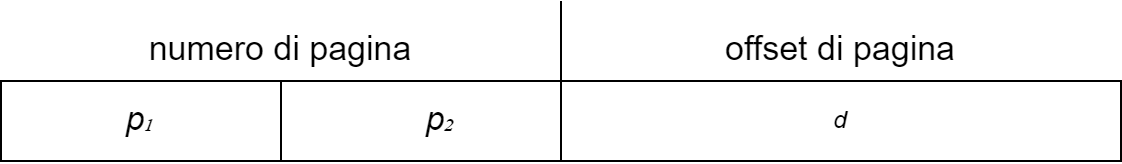
\includegraphics[width =0.8\textwidth]{img/paginazione.png}
            \caption{Divisione dell'indirizzo logico per la paginazione gerarchica}
            \label{fig:my_label}
        \end{figure}
        
        Questa soluzione non è più adatta nel caso di sistemi a 64 bit in quanto la tabella esterna sarebbe nuovamente troppo grande. La soluzione intuitiva è suddividere a tabella in più parti più piccole.
        
        Tuttavia nemmeno questo si dimostra fattibile, e in molti casi andrebbe ulteriormente aumentato il numero di livelli, arrivando in alcuni casi a sistemi di paginazione gerarchica a sette livelli- aumentando molto il numero di accessi alla memoria, e quindi diventando un modello poco desiderabile.
        
    \subsection{Tabella delle pagine invertita}
        Uno svantaggio dei metodi visti fino ad ora è che, dovendo la tabella delle pagine contenere tutti gli indirizzi virtuali di un processo, essa può arrivare a contenere anche milioni elementi, e quindi occupare una grande quantità di memoria fisica.
        
        Per risolvere questo problema si può fare uso della \textbf{tabella delle pagine invertita}. Una tale tabella ha un elemento per ogni pagina reale (o frame). Ciascun elemento è quindi costituito dall'indirizzo virtuale della pagina memorizzata in quel reale frame di memoria e informazioni relative al processo che possiede tale pagina.
        
        Abbiamo quindi una singola tabella per tutta la memoria, che ha un solo elemento per ogni pagina di memoria fisica. Sebbene questo metodo diminuisce lo spazio richiesto per la memorizzazione di tabelle (o in questo caso tabella) delle pagine, aumenta il tempo di ricerca di una pagina nella tabella, siccome la tabella invertita è ordinata per indirizzi fisici, ma i processi ragionano per indirizzi virtuali. Una tale richiesta renderebbe necessario esaminare tutta la tabella nel caso peggiore. Si può ridurre l'entità del problema introducendo una tabella hash, che introduce però un secondo accesso alla memoria (uno alla tabella hash, uno alla tabella della pagine).
        
        Un'altra questione interessante è relativa alla memoria condivisa: un singolo indirizzo non può essere condiviso da più processi impiegando una tabella delle pagine invertita.
        
\section{Swapping dei processi}
    Le istruzioni di un processo e i dati su cui operano devono essere in memoria centrale. Tuttavia un processo o una sua parte può essere temporaneamente rimosso dalla memoria (un'operazione detta \textit{swap out}), spostato in una memoria o partizione ausiliaria e susseguentemente essere ricaricato in memoria (\textit{swap in}). Questo procedimento, detto \textbf{swapping dei processi}, permette ai processi di indirizzare una quantità di indirizzi che eccedono l'effettiva dimensione della memoria fisica, aumentando così il grado di multiprogrammazione.
    
    \subsection{Swapping standard}
        Lo swapping standard è lo spostamento di interi processi fra la memoria centrale e un veloce dispositivo di archiviazione che deve essere abbastanza grande da contenere tutte le porzioni dei processi che devono essere memorizzati nonché fornire accesso diretto alle immagini dei processi memorizzati.
        
        Vanno conservate e quindi memorizzate nella memoria ausiliaria anche le strutture dati relative al processo ed eventualmente ai suoi thread e i metadati del processo, in quanto dovranno essere ripristinati.
        
        Una buona politica di swap out è muovere nella memoria ausiliaria i processi meno usati o comunque usati meno recentemente.

\chapter{Parte Quarta, Capitolo 10: Memoria Virtuale}
\section{Introduzione}
    Gli algoritmi di gestione della memoria visti fino ad ora sono necessari a causa di un importante requisito: le istruzioni da eseguire si devono trovare in memoria fisica. La prima e più banale soluzione è quella di collocare l'intero spazio d'indirizzi logici del processo in memoria fisica.
    
    Questo riduce di molto le dimensioni massime di un programma a valori strettamente collegati alle dimensioni della memoria fisica. Tuttavia, facendo riferimento a programmi reali, notiamo che non è strettamente necessario che tutto il programma si trovi in memoria in un qualsiasi dato momento. Si considerino per esempio casi in cui abbiamo condizioni di errore molto rare, allochiamo più memoria di quanto necessaria in media, o in generale i casi in cui un programma abbia opzioni e casi d'uso rari. Questo è particolarmente palese nei videogiochi: se il giocatore si trova in un livello o zona di una mappa, è totalmente inutile caricare gli altri livelli o tutta la mappa.
    
    Anche nel caso in cui un programma debba essere disponibile nella sua interezza, non caricarlo tutto in memoria porta alcuni vantaggi:
    \begin{itemize}
        \item I programmatori non sono più vincolati dalla quantità di memoria fisica disponibile e possono invece scrivere programmi per uno \textbf{spazio di indirizzi virtuale} molto grande.
        
        \item Il grado di multiprogrammazione aumenta; siccome un programma impiega meno memoria fisica, possiamo avere altri programmi in memoria contemporaneamente.
        
        \item Lo \textit{swapping} richiede meno operazioni di I/O.
    \end{itemize}
    
    Siamo dunque convinti che la possibilità di eseguire un programma che non si trova completamente in memoria apporterebbe molti vantaggi.
    
    La \textbf{memoria virtuale} si basa sul concetto di separazione di memoria fisica e memoria logica percepita dall'utente. L'espressione \textbf{spazio degli indirizzi virtuale} si riferisce alla collocazione dei processi in memoria dal punto di vista logico (o virtuale). Da questo punto di vista lo spazio logico inizia da un certo indirizzo logico, per esempio 0, e si estende in maniera contigua. Come abbiamo visto, le pagine effettive possono essere assegnate ai frame in maniera non contigua, ma la gestione di ciò spetta alla MMU e al sistema operativo. Un altro vantaggio è la condivisione di memoria e file fra diversi processi, tramite la condivisione delle pagine. Questo comporta i seguenti vantaggi:
    \begin{itemize}
        \item Le librerie di sistema possono essere mappate su indirizzi logici di più processi. Così facendo ogni processo vedrà la libreria come appartenente al suo spazio di indirizzi, ma in effetti ci sarà una sola libreria caricata in memoria.
        
        \item In maniera analoga si può condividere la memoria fra più processi. Questo permette a un processo di rendere parte della sua memoria condivisibile da un altro processo, creando così un rapido mezzo di comunicazione.
        
        \item Le pagine possono essere condivise da più processi durante la chiamata di sistema \texttt{fork()}, così da velocizzare la creazione di nuovi processi.
    \end{itemize}
    
\section{Paginazione su richiesta}
    Questa tecnica prevede il caricamento in memoria solo delle pagine richieste all'inizio dell'esecuzione. Durante l'esecuzione, se ulteriori dati saranno richiesti, le pagine corrispondenti saranno caricate dal dispositivo, solitamente la memoria di massa, su cui si trovano.
    
    \subsection{Concetti fondamentali}
        In base a quanto appena visto, quando un processo è in esecuzione alcune delle sue pagine saranno caricate in memoria, mentre altre si troveranno sulla memoria secondaria. Abbiamo quindi bisogno di un supporto hardware per distinguere fra i due casi.
        
        Si può utilizzare lo schema basato sul bit di validità, e considerare il bit come "valido" se la pagina è valida e presente in memoria, come "non valido" se la pagina richiesta non appartiene allo spazio di indirizzamento del processo, oppure se vi appartiene ma è attualmente nella memoria secondaria.
        
        Quando una pagina è contrassegnata come \textit{non valida}, viene generato un \textit{page fault} e il sistema operativo lo gestisce in maniera lineare:
        \begin{enumerate}
            \item Si controlla una tabella interna per questo processo (solitamente conservata insieme al PCB) per verificare se il riferimento fosse valido o meno.
            
            \item Se il riferimento non era valido, si termina il processo. Altrimenti vuol dire che la pagina ancora non è stata caricata e si rimedia caricandola.
            
            \item Si individua un frame libero, per esempio prelevandone uno dalla lista dei frame liberi.
            
            \item Si programma un'operazione per trasferire la pagina desiderata nel frame appena assegnato.
            
            \item Quando la lettura del disco è completata, si aggiornano la tabella interna e la tabella delle pagine per indicare che la pagina si trova attualmente in memoria.
            
            \item Si riavvia l'istruzione interrotta dall'eccezione. A questo punto il processo può procedere come se la pagina fosse sempre stata in memoria.
        \end{enumerate}
        
        Possiamo prendere il caso estremo in cui un processo venga avviato \textit{senza} pagine in memoria. In questo caso tutte le pagine necessarie vengono caricate tramite \textit{page fault}, e si parla di \textbf{paginazione su richiesta pura}.
        
        In alcuni casi potrebbe essere necessario il caricamento di più pagine per una sola istruzione (una per l'istruzione, aggiuntive per i dati). In questo caso le prestazioni sarebbero inaccettabili, ma fortunatamente è una situazione abbastanza rara.
        
        L'hardware di supporto alla paginazione su richiesta è lo stesso necessario per la paginazione e l'avvicendamento dei processi in memoria:
        \begin{itemize}
            \item \textbf{Tabella delle pagine.} Ha la capacità di assegnare a un elemento validità o non validità tramite un bit apposito.
            
            \item \textbf{Memoria secondaria.} Conserva le pagine non allocate in memoria centrale, conservandole su un'area apposita detta \textit{swap space}.
        \end{itemize}
        
        Un requisito importante per la paginazione su richiesta è la possibilità di riprendere l'esecuzione esattamente dal punto in cui è stata interrotta, con stessi registri, stato, etc, a meno della presenza in memoria della pagina richiesta.
        
        Questo è semplice nella maggior parte dei casi, e richiede un lavoro solitamente piccolo (una frazione di istruzione non atomica). Troviamo un problema nel caso in cui un'istruzione possa modificare parecchie locazioni diverse, in quanto in tal caso non è sufficiente limitarsi a riavviare l'istruzione perché le locazioni che ha già modificato potrebbero essere state lasciate in uno stato incoerente. Una \textbf{prima soluzione} consiste nell'accesso alle due estremità dell'area da modificare. I \textit{page fault} possono avvenire solo in questa fase, altrimenti sappiamo che l'intera area è stata caricata e si può procedere a modificarla senza incappare in ulteriori page fault. Una \textbf{seconda soluzione} è quella di copiare le pagine che andremo a modificare in dei registri temporanei, in modo tale da poter ripristinare il loro stato originale in caso di \textit{page fault}.
        
    \subsection{Lista dei frame liberi}
        Ogni volta che avviene un page fault, il sistema operativo deve spostare una pagina dalla memoria secondaria a quella centrale, e per fare ciò deve ovviamente conoscere quali frame sono disponibili ad accomodare pagine.
        
        La maggior parte dei sistemi operativi a questo scopo mantiene una \textbf{lista dei frame liberi}. Vengono spesso allocati con una tecnica nota come \textbf{zero-fill-on-demand}: i frame vengono azzerati su richiesta prima di essere allocati, cancellando il loro precedente contenuto.
        
        All'avvio di un sistema tutta la memoria viene inserita nella lista dei frame liberi e la sua dimensione si riduce man mano che i frame vengono popolati. Quando la sua dimensione si riduce a zero o scende sotto una certa soglia, essa deve essere ripopolata.
        
\section{Copiatura su scrittura}
    Come abbiamo visto, possiamo duplicare l'esecuzione di un processo tramite \texttt{fork()}. La tecnica che abbiamo usato fino ad ora è di duplicare l'intero spazio degli indirizzi del genitore, ma questo può risultare inutile in quanto spesso viene usata una \texttt{exec()} subito dopo.
    
    Adottiamo quindi una tecnica chiamata \textbf{copiatura su scrittura} (\textit{copy-on-write}), che si basa sulla condivisione di pagine fra genitore e figli. Le pagine condivise si contrassegnano come da copiare su scrittura; se un processo (genitore o figlio) scrive su una pagina condivisa, il sistema deve creare una copia di tale pagina.
    
    Notiamo che è necessario contrassegnare come da copiare su scrittura solo le pagine che è effettivamente possibile modificare. Questa tecnica è usata su molti sistemi operativi.
    
\section{Sostituzione delle pagine}
    Fino ad ora abbiamo assunto che ogni pagina di un processo potesse dare origine al più a un page fault, nel momento in cui viene caricata. Tuttavia abbiamo visto che con la paginazione con richiesta, non tutte le pagine devono essere caricate. Questo ci permette di assumere un carico ridotto di I/O, oltre che di aumentare il grado di multiprogrammazione; infatti, con 40 frame, se ogni processo ha dimensione di 10 pagine ma ne caricherà in media la metà, possiamo assumere di caricarne 8 anziché 4, che è un aumento del 100\% del grado di multiprogrammazione.
    
    Tuttavia notiamo subito un problema, nel caso in cui, in un particolare istante di tempo, i processi richiedano più della memoria da noi prevista. Inoltre notiamo che la memoria non è solo riservata solo alle pagine dei processi ma ci sono significative aree di memoria dedicate all'I/O. Questi due problemi rendono più complessa la corretta previsione delle pagine impiegate complessivamente dai processi, e rendono quindi più rischiosa la \textit{sovrassegnazione}.
    
    La \textbf{sovrallocazione} (\textit{over-allocation}) può essere illustrata come segue: durante l'esecuzione di un processo utente si verifica un page fault. A questo punto il sistema operativo va a recuperare dalla memoria di massa la pagina desiderata, ma la lista dei frame liberi è vuota.
    
    Una soluzione consisterebbe nella terminazione del processo utente, tuttavia questo andrebbe contro lo scopo principale della paginazione stessa. In alternativa si può pensare di scaricare un intero processo, liberando tutti i suoi frame. Anche ciò risulta improbabile in quanto lo swapping sandard non è più diffuso a causa del grande overhead richiesto per eseguire lo swap di un intero processo.
    
    I sistemi operativi moderni usano dunque una combinazione di swapping e \textbf{sostituzione di pagina}, che andremo a descrivere di seguito.
    
    \subsection{Sostituzione di pagina}
        La sostituzione delle pagine segue il seguente criterio: se nessun frame è libero, ne viene liberato uno attualmente inutilizzato. È possibile fare ciò scrivendo il suo contenuto nell'area di swap e indicandolo nella tabella delle pagine (e nelle altre tabelle che lo referenziano) come non valido, per indicare che non si trova più in memoria.
        
        La procedura di servizio dell'eccezione di page fault includerà dunque ora un passo intermedio in cui si seleziona una pagina \textbf{vittima} tramite un certo algoritmo e la si scrive nel disco, aggiornando le relative tabelle; quello che abbiamo appena descritto dunque.
        
        Occorre notare che nel caso in cui non ci siano più frame liberi, servono due trasferimenti di pagine, uno swap out per la vittima e uno swap in per la pagina richiesta. Questo \textbf{raddoppia} il tempo richiesto per risolvere il page fault.
        
        Una possibile riduzione di questo problema deriva da un'osservazione: se la pagina non è stata modificata dal momento in cui è stata caricata, non serve ricaricarla sul disco, in quanto \textit{vi sarà già presente}. Questo vale sicuramente per le pagine di sola lettura, ma possiamo implementare un \textbf{bit di modifica} (\textit{modify bit} o \textit{dirty bit}) che inizialmente è posto a 0, e viene posto a 1 se la pagina caricata viene modificata. Nel caso di un \textit{dirty bit} uguale a zero possiamo risparmiarci di fare lo swap out della pagina.
        
        Ci siamo a questo punto convinti dell'utilità della paginazione su richiesta: essa mette a disposizione del programmatore una memoria virtuale molto più grande di quella fisica e separa i due tipi di memoria. Al fine della sua realizzazione però abbiamo bisogno di un \textbf{algoritmo di allocazione dei frame} e di un \textbf{algoritmo di sostituzione delle pagine}. Ciò vuol dire che quando sono presenti due processi in memoria bisogna stabilire quanti frame assegnare a ciascun processo e nel caso di una sostituzione di pagina, occorre selezionare i frame da sostituire.
        
    \subsection{Sostituzione delle pagine secondo l'ordine di arrivo (FIFO)}
        QUesto è l'algoritmo di sostituzione più semplice, e va a sostituire la pagina che si trova da più tempo in memoria. Ovviamente questo algoritmo può essere implementato con una coda FIFO, senza necessità di memorizzare gli istanti di tempo in cui una pagina è stata inserita in memoria.
        
        Per quanto riguarda le prestazioni, questo non è decisamente il miglior algoritmo: è facile da capire, implementare, e i page fault non causano errori, ma non necessariamente la pagina più anziana è la scelta ottimale per la sostituzione.
        
        Introduciamo anche l'\textbf{anomalia di Belady}: nonostante possa risultare logico che l'aumento di frame disponibili corrisponda a una diminuzione dei page fault, talvolta viene osservato sperimentalmente il contrario.
        
    \subsection{Sostituzione ottimale delle pagine}
        Dopo la scoperta dell'anomalia di Belady è iniziata la ricerca di una algoritmo ottimale per la sostituzione delle pagine, ossia l'algoritmo che non presenta mai tale anomalia e allo stesso tempo non presenta mai l'anomalia di Belady. Questo algoritmo esiste ed è chiamato OPT o MIN, e consiste nel: \textit{sostituire la pagina che non verrà usata per il periodo di tempo più lungo}.
        
        Questo algoritmo, per definizione, è ottimo, anche se difficile da realizzare in quanto richiede la conoscenza futura della successione dei riferimenti, una situazione analoga all'algoritmo SJF nell'ambito dello scheduling della CPU. Per questo motivo è usato perlopiù in esempi e come metro di paragone per altri algoritmi.
        
    \subsection{Sostituzione delle pagine usate meno recentemente (LRU)}
        L'algoritmo \textbf{LRU} (\textit{least recently used}) tenta di approssimare quello ottimale, andando a sostituire la pagina che \textbf{non è stata usata per il periodo più lungo}.
        
        Possiamo implementare ciò associando a ciascuna pagina l'istante in cui è stata usata per l'ultima volta. Nonostante alcune problematiche, questo algoritmo resta uno dei migliori anche se sub-ottimo, e viene spesso considerato valido e utilizzato nella pratica. Le difficoltà principali sono relative alla sua implementazione, in quanto ordinare i frame in base al loro ultimo utilizzo può richiedere una considerevole assistenza da parte dell'hardware. Si possono realizzare le due seguenti soluzioni:
        \begin{itemize}
            \item \textbf{Contatori.} Si inizializza un contatore che viene incrementato a ogni riferimento alla memoria. Ogni volta che si fa riferimento a una pagina, si copia il contenuto del contatore in una apposita variabile, e la pagina meno recentemente utilizzata sarà quella con il valore di questa variabile più basso. Questo implica però la ricerca della pagina meno recentemente utilizzata e una scrittura in memoria per ogni accesso alla memoria.
            
            \item \textbf{Stack.} Il secondo metodo implica uno stack, e il posizionare l'elemento appena usato in cima a quest'ultimo. In tal modo l'elemento più recentemente utilizzato si trova in cima allo stack, quello meno recentemente utilizzato in fondo. Siccome gli elementi appena utilizzati si trovano al centro dello stack, quest'ultimo viene spesso implementato come una lista doppiamente concatenata.
        \end{itemize}
        
        Né la sostituzione ottimale né quella LRU sono soggetti all'anomalia di Belady, in quanto facenti parte di una classe chiamata \textbf{algoritmi a stack}.
        
        Si noti tuttavia che questi algoritmi sarebbero impossibili senza un certo supporto hardware, in quanto sono necessari aggiornamenti di strutture dati a ogni accesso alla memoria, il che causerebbe un sovraccarico eccessivo.
        
    \subsection{Sostituzione delle pagine per approssimazione a LRU}
        Sono pochi i sistemi di calcolo che dispongono dell'hardware necessario per implementare un vero algoritmo di sostituzione basato su LRU. Tuttavia un algoritmo di tipo FIFO è troppo impreciso.
        
        Molti sistemi offrono un aiuto: il \textbf{bit di riferimento}. Questo è un bit inizialmente impostato a zero per tutte le pagine, e che viene impostato a uno quando una pagina viene referenziata. Così facendo possiamo sapere a quali pagine abbiamo fatto riferimento, ma non in che ordine. Ciò è la base per molti algoritmi che approssimano il modello LRU.
        
        \paragraph{Algoritmo con bit supplementari di riferimento}
            Possiamo registrare il bit di riferimento a intervalli regolari. Supponiamo per esempio di avere un byte per ogni pagina.
            
            A intervalli regolari in interruzione trasferisce il controllo al sistema operativo, che registrerà il bit di controllo di ciascuna pagina nel bit più significativo del vettore appena definito. In questo modo sapremo che la pagina con associato il byte 00000000 non è stata usata da otto periodi di tempo, e per esempio che la pagina con il byte 10110101 è stata usata più recentemente della pagina con byte 01110111. Interpretando questi byte come interi senza segno, possiamo prendere quello minore come migliore approssimazione del LRU.
            
            Ovviamente il numero di bit usati può variare e dipende dall'hardware disponibile, e nel caso limite in cui sia zero, si parla di \textbf{algoritmo di sostituzione con seconda chance}.
            
        \paragraph{Algoritmo con seconda chance}
            Questo semplice algoritmo si basa sull'algoritmo che usa una coda FIFO. Una volta selezionato l'ultimo elemento, si controlla però il bit di riferimento: se questo è 0 si sostituisce la pagina, se è 1 gli viene data una seconda chance e si passa all'elemento successivo della coda.
            
            Quando a una pagina viene data una seconda chance si azzera il suo bit di riferimento e si aggiorna il suo istante di arrivo al momento corrente.
            
            Una possibile implementazione può avvenire tramite una coda circolare, e viene detta \textbf{a orologio} (\textit{clock}), in cui un puntatore (lancetta) indica la prima pagina da sostituire. A ogni riferimento, si fa avanzare la lancetta finché non si trova un bit di riferimento 0, azzerando inoltre il bit dell'elemento appena visitato. Una volta trovata la pagina vittima, si inserisce al suo posto la nuova pagina.
            
            Si noti che nel caso peggiore, ossia di tutti i bit di riferimento impostati a 1, viene visitata tutta la cosa e tutti i bit vengono impostati a 0.
            
        \paragraph{Algoritmo con seconda chance migliorato}
            L'algoritmo precedentemente descritto si può migliorare considerando i bit di riferimento e modifica una coppia ordinata, con cui si possono ottenere le seguenti quattro classi:
            \begin{enumerate}
                \item (0, 0). Né recentemente usato né modificato - migliore pagina da sostituire.
                
                \item (0, 1). Non recentemente usato ma modificato - pagina non ottima da sostituire in quanto dovrà essere scritta in memoria.
                
                \item (1, 0). Recentemente usato ma non modificato - probabilmente sarà usato di nuovo a breve.
                
                \item (1, 1). Recentemente usato e modificato - probabilmente sarà usato di nuovo e dovrà inoltre essere scritto in memoria.
            \end{enumerate}
            
            Si usa la visita a orologio ma si sostituisce la prima pagina con classe minima non vuota. Si noti che si dovrebbe poter visitare l'intera coda più volte prima di eseguire una sostituzione. La differenza principale col metodo precedentemente descritto è che qui si prende in considerazione il bit di modifica, cercando quindi di diminuire anche il numero di I/O.
            
    \subsection{Sostituzione delle pagine basata su conteggio}
        Potremmo pensare di usare un contatore dei riferimenti fatti a ciascuna pagina, e sviluppare i due seguenti schemi:
        \begin{itemize}
            \item \textbf{Algoritmo di sostituzione delle pagine meno frequentemente usate} (\textit{least frequently used}, LFU); si sostituisce la pagina con il contatore più basso. Il ragionamento dietro ciò è che una pagina poco usata deve avere un contatore basso. Tuttavia incorriamo in un problema nel caso in cui una pagina venga utilizzata molto intensamente alla creazione di un processo per poi venire messa da parte. Una possibile soluzione è quella di implementare un processo di \textit{aging}, per esempio spostando a destra i bit del contatore a intervalli regolari.
            
            \item \textbf{Algoritmo di sostituzione delle pagine più frequentemente usate} (\textit{most frequently used}, MFU); si basa sull'idea che, probabilmente, la pagina con il contatore più basso è appena stata inserita e quindi dovrà essere usata ancora.  
        \end{itemize}
        
\section{Allocazione dei frame}
    Affrontiamo ora il problema dell'allocazione dei frame. Avendone un numero limitato e più processi che li richiedono, la scelta di quanti frame allocare a quale processo è importante.
    
    Come caso base possiamo prendere una combinazione di paginazione su richiesta pura e uno degli algoritmi di sostituzione visti, ma ci sono molte variazioni di questa semplice strategia, ma la base è chiara: si assegna al processo utente qualsiasi frame libero.
    
    \subsection{Numero minimo di frame}
        Le strategie di allocazione di frame sono soggette a parecchi vincoli. Per esempio, non si possono allocare più frame di quanti ne siano disponibili, e allo stesso tempo è necessario allocare un numero minimo di frame. Esaminiamo quest'ultimo requisito in maggior dettaglio.
        
        Il motivo principale di un limite minimo di pagine è legato alle prestazioni. Ovviamente al diminuire del numero di frame, ogni processo degrada in prestazioni, a causa dell'aumento di page fault. Inoltre, un'istruzione che incorre in un page fault deve essere riavviata. È necessario quindi avere un numero di frame che possa accomodare ogni singola istruzione di un dato processo.
        
        Il numero minimo di frame per un processo è definito dall'architettura, mentre quello massimo dalla quantità di memoria disponibile. Fra questi due valori vi è ampio spazio di scelta.
    
    \subsection{Allocazione globale e allocazione locale}
        Un altro importante fattore che riguarda l'assegnazione di frame, è la sostituzione delle pagine. Nel caso in cui ci siano più processi in competizione per i frame, gli algoritmi di sostituzione di pagine si possono classificare in due categorie generali: \textbf{sostituzione globale} e \textbf{sostituzione locale}. La sostituzione globale permette a un processo che necessita di un frame di sceglierlo dall'insieme completo dei frame; può quindi sottrarre frame ad altri processi. La sostituzione locale permette a un processo di scegliere un frame solo e soltanto dal suo insieme di frame.
        
        Si consideri per esempio uno schema di assegnazione di frame con priorità: potremmo consentire a un processo con priorità più alta di sottrarre frame a qualsiasi processo con priorità più bassa.
        
        La sostituzione locale rischia di non rendere disponibili a un processo pagine di memoria poco usate, e difatti spesso la paginazione globale è più efficiente ed utilizzata; vale la pena notare un problema che la affligge: un processo non può controllare il proprio tasso di page fault, in quanto l'insieme di pagine che si trova in memoria non dipende solo dal processo stesso ma anche dagli altri processi.
        
        Una possibile \textbf{implementazione} sta nel riciclare l'idea della lista dei frame liberi. Tuttavia, anziché aspettare che la lista si svuoti per iniziare a fare sostituzioni, aspettiamo che scenda sotto una certa soglia. Lo scopo è quello di mantenere la quantità di memoria libera sopra una certa soglia. Quando si scende al di sotto di questa soglia vengono avviate delle routine kernel, solitamente chiamate \textbf{reapers}, che iniziano a recuperare memoria da tutti i processi (in genere escludendo il kernel stesso). Quando la memoria disponibile raggiunge una \textit{soglia massima}, i reaper si fermano, per poi ripartire una volta superata di nuovo la \textit{soglia minima}.
        
        I reaper possono impiegare qualsiasi algoritmo di sostituzione di pagina, ma solitamente adottano un algoritmo di approssimazione di LRU. Possono inoltre cambiare algoritmo o adottare politiche più aggressive quando non è in grado di mantenere la lista dei frame liberi al di sopra della soglia minima.
        
    \subsection{Accesso non uniforme alla memoria}
        Fino ad ora abbiamo assunto che diverse parti della memoria all'interno dello stesso sistema fossero uguali, o che comunque vi si potesse accedere nello stesso modo. In \textbf{sistemi con accesso non uniforme alla memoria (NUMA)}, dotati di più CPU, non è così.
        
        Su questi sistemi, una CPU può accedere più velocemente a una certa area di memoria rispetto alle altre, che definiamo memoria locale di quella CPU. Nonostante i sistemi NUMA siano, senza eccezioni, più lenti dei sistemi in cui tutti gli accessi alla memoria sono trattati nello stesso modo, vale la pena di considerarli in quanto possono raggiungere livelli maggiori di throughput e parallelismo.
        
        Un sistema conscio dell'architettura NUMA dovrà infatti comportarsi di conseguenza: quando un processo incorre in un page fault, è preferibile caricare la pagina nel frame più "vicino" a lui. Se lo scheduler della CPU tenta di schedulare un certo processo su una certa CPU e il sistema di gestione di memoria virtuale tenta di allocare i frame sull'area di memoria più vicina a quella determinata CPU, avremo un numero minore di page fault e quindi un aumento delle prestazioni.
        
\section{Thrashing}
    Si consideri la situazione in cui il numero di frame non è "sufficiente". Andremo a sostituire pagine che saranno tuttavia appartenenti a processi attivi, e quindi saranno subito richieste di nuovo, causando moltissimi page fault.
    
    Questa intensa paginazione è nota come \textit{thrashing}, e causa una degradazione rapida e notevole delle prestazioni del sistema.
    
    \subsection{Cause del thrashing}
        Una causa di thrashing può essere l'aumento incontrollato del grado di multiprogrammazione. Eseguendo una quantità eccessiva di processi si tocca un tetto oltre il quale il numero di frame a disposizione non riesce ad accomodare tutti i processi e quindi inizia un'attività intensa di paginazione, che fa decadere le performance dell'intero sistema.
        
        Si può attenuare questo problema impedendo a un processo entrato in thrashing di sottrarre frame a un altro processo, cosa che corrisponde a un \textbf{algoritmo di sostituzione locale}.
        
        Per evitare totalmente queste situazioni occorre dare a un processo tutti i frame di cui ha bisogno. Ci sono diversi approcci per stimare questo valore. L'approccio del \textbf{working-set} comincia osservando quanti frame il processo sta effettivamente usando, approccio che definisce il \textbf{modello di località} d'esecuzione del processo.
        
        Il modello di località stabilisce che un processo, durante la sua esecuzione, si muove di località in località, dove la località è un insieme di pagine usate attivamente insieme. Se si allocano abbastanza frame per accomodare le località attuali del processo, finché queste non verranno modificate non avverranno altri page fault.
        
        
        Questo modello è, si noti, l'assunzione fatta fino ad ora per analizzare il caching. Quest'ultimo sarebbe infatti inutile nel momento in cui gli accessi ai dati fossero casuali, anziché strutturati in località.
        
    \subsection{Modello del working set}
        Come già accennato, questo modello fa riferimento all'ipotesi di località di un processo. Questo modello usa un parametro, $\Delta$, come \textbf{finestra del working set}. L'idea consiste semplicemente nell'aggiungere al working set le pagine attivamente in uso, e rimuoverle dopo $\Delta$ unità di tempo.
        
        Un $\Delta$ troppo piccolo potrebbe non includere l'intera località, mentre un $\Delta$ troppo grande implica la sovrapposizione di più località. Nel caso limite, un $\Delta$ infinito fa coincidere il working set con l'insieme di pagine referenziate durante l'intera esecuzione del processo.
        
        Data la natura dinamica del working set, la difficoltà principale sta nel tenere traccia dei suoi elementi. A ogni riferimento alla memoria, a un'estremità appare un elemento nuovo, mentre l'elemento più vecchio fuoriesce dall'altra estremità. Una pagina si trova nel working set se uno qualsiasi dei suoi elementi referenzia la pagina stessa.
        
    \subsection{Frequenza dei page fault}
        Il modello del working set ha avuto successo ed è utile conoscerlo, ma appare una soluzione alquanto goffa al problema del thrashing. Una strategia più diretta è quella basata sulla \textbf{frequenza dei page fault} (\textit{page fault frequency}, PFF).
        
        Il problema specifico è la prevenzione del thrashing. Possiamo pensare di monitorare la frequenza dei page fault per un dato processo. Se questa è alta, il processo ha bisogno di più frame, mentre se è bassa c'è un'abbondanza di frame.
        
        Possiamo per esempio stabilire una soglia superiore di frequenza di page fault oltre la quale a un processo vengono dati frame aggiuntivi, e una inferiore sotto la quale gli vengono sottratti frame.
        
        Come nel caso del working set, se la frequenza di page fault per un processo è alta e non disponiamo di ulteriori frame, potrebbe essere necessario eseguire uno swap out del processo, liberando così tutti i suoi frame.
        
\section{Altre considerazioni}
    Le due scelte principali nella progettazione dei sistemi di paginazione sono l'algoritmo di sostituzione e la politica di allocazione discusse precedentemente, ma vanno fatte anche altre considerazioni.
    
    \subsection{Dimensione delle pagine}
        È raro che chi progetta un sistema operativo debba o possa scegliere la dimensione delle pagine. Tuttavia è una cosa importante da tenere in conto durante la progettazione di un nuovo calcolatore. Non esiste una dimensione univocamente migliore ma sappiamo che sono sempre potenze di due, solitamente comprese fra $2^{12}$ (4096) e $2^{22}$ (4.194.304) byte.
        
        Un fattore da tenere in considerazione per esempio è la \textbf{dimensione della tabella delle pagine}. Per pagine più piccole la tabella sarà più grande (dovrà indicizzare più pagine), e dovendo ogni processo avere in memoria suddetta tabella, ci conviene avere pagine grandi. Tuttavia pagine di grandi dimensioni causano una maggiore frammentazione interna.
        
        Un secondo fattore è il \textbf{tempo di richiesto per leggere o scrivere} una pagina, soprattutto su dispositivi di memorizzazione meccanici. Il tempo di posizionamento e di latenza dominano quello effettivo di scrittura o lettura, rendendo preferibili pagine più grandi. Pagine piccole tuttavia migliorano le prestazioni di I/O totale, in quanto garantiscono una maggiore \textbf{risoluzione}; ciò vuol dire che di un processo si possono caricare solo le parti richieste con piccole pagine, mentre con pagine grandi occorre trasferire e allocare non solo quanto è necessario, ma tutto quanto è nella pagina.
        
        Ancora, il \textbf{numero di page fault} aumenta drasticamente con pagine di piccole dimensioni, rendendo preferibili grandi pagine in questo riguardo.
        
        Non esiste dunque una risposta definitiva alla dimensione delle pagine, in quanto alcuni fattori sono a favore di dimensioni minori, altri viceversa favoriscono dimensioni piccole. Tuttavia, storicamente, la preferenza è per pagine più grandi.
        
    \subsection{Portata del TLB}
        Il \textbf{tasso di successi} (\textit{hit ratio}) di un TLB si riferisce alla percentuale di indirizzi virtuali correttamente tradotti dal TLB anziché dalla tabella della pagine. Questo numero è chiaramente proporzionale alla dimensione del TLB stesso e quindi sarebbe preferibile aumentarne le dimensioni. Tuttavia la memoria associativa alla base di un TLB è costosa e consuma molta energia.
        
        Una metrica collegata al tasso di successi viene detta \textbf{portata del TLB} (\textit{TLB reach}) ed è data semplicemente dal numero di elementi del TLB stesso moltiplicata per la dimensione delle pagine.
        
        È quindi ovvio che per aumentare la TLB reach dobbiamo aumentare uno dei due fattori che la compongono. Come abbiamo visto, pagine più grandi causano frammentazione interna. Una possibile soluzione sta nell'utilizzo di pagine di diverse dimensioni. Su Linux per esempio, la dimensione standard di una pagina è 4Kb; tuttavia permette di utilizzare pagine denominate \textit{huge page}, che possono arrivare a dimensioni di 2MB.
        
        Nell'architettura ARMv8, ciascun elemento del TLB contiene un \textbf{bit di contiguità}, che indica che l'elemento mappa blocchi di memoria contigua. La portata del TLB è così aumentata, in quanto blocchi contigui possono essere mappati su un singolo elemento del TLB.
        
    \subsection{Tabella delle pagine invertita}
        Questo concetto visto in precedenza si sposa male con la paginazione. Nel caso di page fault infatti si deve necessariamente far riferimento a una tabella della pagine esterna per ciascun processo, che forniscono le informazioni necessarie sullo spazio degli indirizzi logici di ciascun processo.
        
        Fortunatamente queste tabelle sono necessarie solo quando avviene un page fault. C'è da considerare che un primo page fault può generarne un secondo quando viene caricata in memoria la tabella delle pagine esterna, problema che richiede un'accurata gestione da parte del kernel.
        
    \subsection{Struttura dei programmi}
        Abbiamo detto che la paginazione su richiesta deve essere trasparente ai programmi utenti; spesso essi non saranno nemmeno a conoscenza della natura paginata della memoria. Tuttavia, talvolta questa conoscenza può portare a scrivere programmi più efficienti.

\chapter{Parte Quinta, Capitolo 11: Memoria di massa}
\section{Struttura dei dispositivi di memorizzazione}
    I \textbf{dischi magnetici} e i \textbf{dispositivi NVM} (\textit{non volatile memory}) costituiscono i principali supporti di memoria secondaria nei moderni computer. Andiamo a descriverne la struttura e in che modo i sistemi operativi riescano a tradurre le loro proprietà fisiche in memoria logica tramite la mappatura degli indirizzi.
    
    \subsection{Dischi rigidi}
        Concettualmente, la struttura di un disco rigido è abbastanza semplice: sono simili a dei cd divisi in \textit{settori}, a loro volta organizzati \textit{tracce}. Se prendiamo tutte le tracce corrispondenti verticalmente, una per ogni disco, abbiamo un \textit{cilindro}.
        
        Le dimensioni del settore sono state per molto tempo di 512 byte, ma dal 2010 i produttori hanno iniziato a migrare verso una soluzione di 4KB per settore.
        
        \begin{figure}[h]
            \centering
            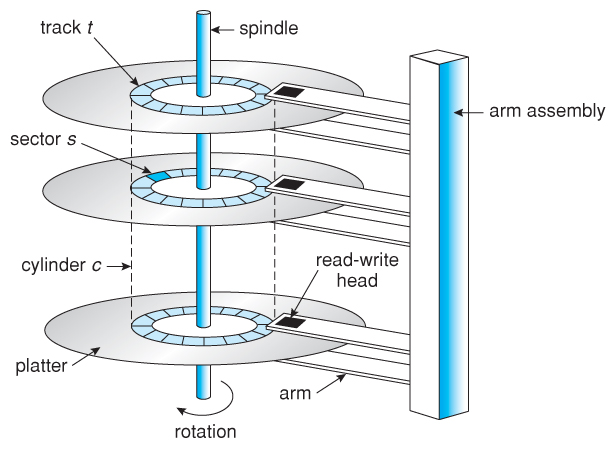
\includegraphics[width = 0.8\textwidth]{img/hd.jpg}
            \caption{Struttura di un disco rigido}
            \label{fig:my_label}
        \end{figure}
        
        \paragraph{Aspetto meccanico.} Quando un disco è in funzione, un motore lo fa ruotare ad alta velocità, la quale è spesso espressa in termini di RPM, ossia giri al minuto, i quali possono variare da 5400 a 15000. Un altro aspetto relativo alle prestazioni è il \textbf{tempo di posizionamento}, composto dal tempo necessario a spostare il braccio del disco in corrispondenza del cilindro desiderato, e il tempo necessario affinché il settore desiderato si posti, tramite la rotazione, sotto la testina.
        
        Il fenomeno dell'\textbf{urto della testina} avviene quando la testina danneggia il disco magnetico, e comporta la sostituzione dell'intera unità di memoria e la perdita dei dati.
        
    \subsection{Dispositivi NVM}
        I dispositivi NVM sono elettrici anziché meccanici, e questo permette delle performance e una durabilità maggiori rispetto a quelli classici. Una grande parte di essi sono costituiti da un controllore e da diversi chip di memoria a semiconduttore NAND flash. Esistono altre tecnologie ma sono molto meno popolari.
        
        Questi dispositivi sono spesso inseriti in contenitori simili a unità disco, e per questo motivo vengono spesso chiamati \textbf{dischi a stato solido}, o \textbf{SDD} (\textit{solid state drive}). In altri casi può assumere altre forme, come le chiavette USB o un chip installato direttamente sulla scheda madre, come sugli smartphone. In ogni caso, possiamo discutere di questi dispositivi alla stessa maniera, in quanto si comportano allo stesso modo.
        
        Come abbiamo detto, questi dispositivi sono \textbf{più efficienti} delle controparti classiche in quanto non hanno bisogno di posizionamento meccanico, più resistenti ai guasti per lo stesso motivo e consumano meno energia. D'altro canto sono più costosi e tendono ad avere una capacità minore. Questi fattori sono tuttavia in costante miglioramento col passare degli anni.
        
        In funzione dell'alta velocità di trasferimento di questi dispositivi, l'interfaccia bus può costituire un \textbf{bottleneck} non indifferente al throughput, e quindi alcuni dispositivi NVM si connettono direttamente al bus di sistema.
        
        Le caratteristiche dei semiconduttori NAND portano tuttavia \textbf{nuove sfide}: nonostante sia possibile eseguire scritture a livello di pagina, non è possibile sovrascrivere dati, e quindi occorre eseguire una cancellazione (operazione molto costosa, anche perché si verifica a livello di blocchi di diverse pagine) prima di riscrivere. In una certa misura ciò è limitato da un certo livello di parallelismo offerto da questi dispositivi, grazie ai molti \textbf{datapath} di cui dispongono.
        
        Inoltre l'\textbf{usura} dei dispositivi NVM dipende dall'utilizzo: in media un semiconduttore NAND si deteriora e diventa inutilizzabile dopo 100.000 cicli, e la durata di un tale dispositivo non viene espressa in anni ma in base al numero di scritture al giorno.
        
        Queste limitazioni hanno portato allo sviluppo di algoritmi di miglioramento che fortunatamente non sono a carico del sistema operativo ma del dispositivo, rendendolo dunque più intelligente.
        
\section{Gestione delle unità di memoria secondaria}
    Il sistema operativo è responsabile di alcuni aspetti della gestione delle unità di memoria a disco: discutiamo in questo paragrafo l'inizializzazione del dispositivo, l'avviamento del sistema dal dispositivo e la gestione di blocchi difettosi.
    
    \subsection{Formattazione del disco, partizioni e volumi}
        Un dispositivo di memorizzazione nuovo non contiene nulla, ma deve essere inizializzato e diviso in settori che possano essere scritti o letti dal controllore, processo chiamato \textbf{formattazione di basso livello} o \textbf{formattazione fisica}. Essa riempie il dispositivo con una speciale struttura dati per ogni locazione di memorizzazione, la quale consiste tipicamente di un'intestazione, un'area per i dati e una coda. La prima e l'ultima contengono informazioni usate dal controllore del disco come per esempio il numero del settore e un codice per la correzione di errori.
        
        La formattazione fisica è spesso parte del processo di produzione dell'hardware, in maniera che il produttore possa testare il disco. Una delle scelte fatte in questa fase è la dimensione dei settori, spesso ristretta a poche opzioni come 512 byte e 4 Kb. La maggiore dimensione di settori implica la presenza di meno settori per ogni striscia, ma anche una minor quantità di code e intestazioni, e quindi in definitiva più spazio di archiviazione.
        
        Prima di usare il disco come contenitore per i file, il sistema operativo deve prima registrare le sue strutture dati sullo stesso, cosa che fa in tre passi:
        \begin{itemize}
            \item Suddividere il disco in uno o più blocchi di blocchi, dette \textbf{partizioni}. Il sistema può trattare ogni partizione come se fosse un dispositivo a sé, e infatti spesso ciò avviene nella misura in cui viene installato un intero sistema operativo su ogni partizione.
            
            \item Creazione e gestione del volume. A volte ciò è implicito, come quando un file system viene inserito direttamente in una partizione la quale è poi pronta a essere montata e usata, altre volte è esplicito.
            
            \item La \textbf{formattazione logica}, ossia la creazione del file system; il sistema operativo registra nel dispositivo le strutture dati iniziali relative al file system, le quali possono includere descrizioni dello spazio libero, dello spazio occupato e una cartella iniziale vuota.
        \end{itemize}
        
        Alcuni sistemi operativi permettono a certi programmi di impiegare una partizione del disco come un grande array sequenziale di blocchi logici, non contenente alcuna struttura dati relativa al file system. Questo array è detto \textbf{disco di basso livello} (\textit{raw disk}). Il relativo I/O si chiama \textbf{I/O di basso livello}. Una tale struttura può per esempio essere usata come spazio di swap. Nonostante alcuni programmi potrebbero essere più efficienti tramite un tale tipo di accesso, la maggior parte preferiscono usare il file system fornito anziché farsi carico della gestione dei dati.
        
    \subsection{Blocco d'avviamento}
        Affinché un computer possa entrare in funzione, all'avvio o riavvio, è necessario che esegua un programma iniziale. Di solito questo \textit{bootstrap} è piuttosto semplice. Esso è spesso memorizzato nel \textit{firmware} ed è posizionato su una memoria NVM sulla scheda madre, e mappato su una locazione di memoria nota.
        
        Il piccolo programma di avviamento del bootstrap, il \textit{bootstrap loader}, è capace di caricare il bootstrap completo, il quale a sua volta è più complesso e può caricare tutto il sistema operativo e inizializzare ogni aspetto del computer.
        
    \subsection{Blocchi difettosi}
        Le unità a disco sono strutturalmente soggette a guasti, a causa delle varie parti meccaniche mobili. Alcuni di questi possono portare a errori irreparabili, e causare quindi il cambio dell'intera unità, ma possiamo anche trovare \textbf{blocchi difettosi} (\textit{bad blocks}). Ciò è così comune che la maggior parte delle unità messe in commercio già contengono blocchi difettosi.
        
        Se si trovano blocchi difettosi durante la formattazione, essi possono essere marcati come non utilizzabili. Se un blocco diviene difettoso durante l'uso del disco, deve essere lanciato un programma specifico che li individua. Spesso il suo contenuto viene perso.
        
        Unità a disco più complesse hanno strategie più raffinate per trattare i blocchi difettosi: li individua e li lista già in fase di produzione, e questa lista viene tenuta aggiornata per tutta la durata operativa dell'unità. Inoltre viene tenuta una lista di blocchi nascosti che possono essere sostituiti logicamente a quelli difettosi. Quest'ultima strategia è nota come \textbf{accantonamento dei settori} (\textit{sector sparing} o \textit{forwarding}).
        
        Questo potrebbe inficiare sulle prestazioni, e infatti molti dischi tengono blocchi di riserva per ogni cilindro, in maniera tale da non dover riposizionare la testina.
        
        Un'alternativa è la \textbf{traslazione dei settori}, o \textit{sector slipping}: se il blocco 10 è malfunzionante e il primo blocco di riserva libero è il 140, tutti i settori dal 10 al 139 vengono spostati in avanti di una posizione.
        
        In generale, un errore è \textit{reversibile} quando possiamo in qualche modo recuperare il contenuto del blocco, mentre è \textit{irreversibile} quando ciò non si può fare e dobbiamo quindi ricorrere a un backup, operazione da eseguire manualmente.
        
        Anche i dispositivi NVM possono avere pagine difettose, ma in questo caso la soluzione non incide sul tempo di riposizionamento, e quindi gli algoritmi sono più semplici ed efficienti.
        
\section{Gestione dell'area di avvicendamento (swap space)}
    Abbiamo già parlato dello swapping: nel momento in cui ci siano troppi processi e la memoria si riempia, le prestazioni degradano e diventa necessario fare lo \textit{swap in} di processi per permettere a nuovi processi di entrare in memoria; nella pratica ciò è molto raro, in quanto fare lo \textit{swap out} di interi processi è inutile e dispendioso. Si manda in area di avvicendamento piuttosto una parte di un processo espressa in pagine, combinando quindi questo concetto con tecniche di memoria virtuale.
    
    La \textbf{gestione dell'area di swap} è un altro compito di basso livello del sistema operativo. Siccome come area di swap viene spesso usata un'unità a disco, il suo uso riduce notevolmente le prestazioni. Lo scopo è quindi realizzare un'area di swap che fornisca il miglior throughput possibile.
    
    \subsection{Uso dell'area di swap}
        L'uso di quest'area dipende dal sistema operativo: alcuni possono memorizzarvi le immagini di interi processi, altri solo delle pagine. Ne deriva che lo spazio richiesto da quest'area è molto variabile, dai megabyte ai gigabyte.
        
        Si noti che una stima per eccesso è meno dannosa di una per difetto, in quanto un'area di avvicendamento troppo grande spreca memoria altrimenti utilizzabile per i file, mentre una troppo piccola potrebbe richiedere la soppressione forzata di processi nel caso di esaurimento.
        
    \subsection{Collocazione dell'area di swap}
        Questa area può essere collocata all'interno del normale file system o in una partizione dedicata. Nel primo caso possiamo usare le ordinarie operazione per cercarla, darle un nome, etc, come gli altri file nel file system.
        
        In caso contrario abbiamo una \textit{raw partition} senza alcun file system, ma a cui  è più facile e veloce accedere. Questo causa una maggiore frammentazione, della quale tuttavia non ci preoccupiamo molto in quanto i file sulla partizione di swap hanno vita breve. Difatti questi vengono eliminati al riavvio del PC.
        
\section{Connessione dei dispositivi di memorizzazione}
    I calcolatori accedono alla memoria secondaria in tre modi: tramite un dispositivo collegato alla macchina, alla rete o tramite un dispositivo cloud.
    
    \subsection{Memoria secondaria connessa alla macchina}
        Alla memoria connessa alla macchina si accede dalle porte di I/O locale, le quali utilizzano diverse tecnologie, la più popolare delle quali è SATA.
        
        In architetture di fascia alta e server ci si può avvalere di diverse tecnologie come cavi di rame e fibra ottica.
        
        Anche i dispositivi sono omogenei, come per esempio unità a disco, Blu-Ray, dispositivi NVM.
        
    \subsection{Memoria secondaria connessa alla rete}
        Un \textbf{dispositivo NAS} (\textbf{network-attached storage}) fornisce accesso a spazio di archiviazione tramite la rete. Può essere costituito da un dispositivo specializzato o da un semplice computer che fornisce il suo spazio di memoria ad altri computer connessi attraverso la rete.
        
    \subsection{Memoria secondaria su cloud}
        Alcuni fornitori di servizi cloud forniscono spazio di archiviazione remoto, che prende il nome di \textit{cloud storage} ed è accessibile tramite Internet o altre reti WAN. Al contrario dei dispositivi NAS, il cloud storage presenta modalità di accesso basate su API, questo per far fronte alla maggiore latenza rispetto a una rete LAN e alla maggiore possibilità di perdita della connessione.
    
    \subsection{Storage-area network e storage array}
        Un problema dei sistemi di memoria connessi alla rete è che competono con gli altri servizi per la banda, dovendone occupare una quantità considerevole per le operazioni di I/O.
        
        Una \textbf{storage-area network (SAN)} è una rete privata che impiega protocolli specifici tra i server e le unità di memoria secondaria. Essa è molto flessibile e può per esempio connettersi a molte macchine, assegnare più memoria a quali ne abbiano bisogno, eccetera.
        
        Uno \textbf{storage array} è un dispositivo che può includere porte SAN, di rete o entrambe. Contiene unità per memorizzare dati, un controllore e permette l'accesso tramite la rete. I controllori sono composti da CPU, memoria e software e regolano le funzionalità dell'array, compresi protocolli, snapshot, duplicazione, crittografia, etc.
        
\section{Strutture RAID}
    Con il diminuire del costo delle unità di memorizzazione, possiamo avere più dischi nello stesso sistema, potenzialmente capaci di operare in parallelo. Questo presenta l'opportunità di memorizzare i dati in maniera ridondante, per diminuire la sensibilità ai fault. Ci sono vari metodi di organizzazione di queste strutture, noti come \textbf{batterie ridondanti di dischi} (\textit{redundant array of indipendent disks}, \textbf{RAID}).
    
    Storicamente una struttura RAID veniva impiegata per motivi economici (infatti la \textit{I} stava per \textit{inexpensive}), mentre oggi il motivo principale è l'affidabilità.
    
    \subsection{Miglioramento dell'affidabilità tramite la ridondanza}
        In una batteria di dischi, la possibilità di guasto di un qualsiasi disco è certamente più alta della probabilità di guasto di un disco preso singolarmente. Per questo viene introdotta una certa \textbf{ridondanza}, ossia la memorizzazione di informazioni non necessarie ma che in caso di guasto possono essere utili a ricostruire i dati persi. La stessa tecnica si può attuare per dispositivi NVM, ma non avendo parti meccaniche, questi ultimi sono meno soggetti ai guasti.
        
        Il metodo più semplice ma più costoso di ridondanza è il \textbf{mirroring}: ogni scrittura effettuata su un disco viene effettuata anche su un secondo disco identico. Perdiamo i dati solo nel caso si guasti un primo disco e prima della sostituzione si guasti anche il secondo, evento generalmente molto improbabile.
        
        Un problema particolarmente sentito è il calo di alimentazione elettrica: in questo caso i due dischi gemelli possono essere lasciati in uno stato incoerente se stavano scrivendo lo stesso dato sullo stesso blocco. Una possibile soluzione è scrivere prima su un disco e in secondo momento sul secondo disco. Un'altra soluzione è l'impiego di una \textbf{NVRAM}, \textit{non volatile RAM}, la quale è protetta dalla perdita di dati anche in caso di mancanza di corrente elettrica.
        
    \subsection{Miglioramento delle prestazioni tramite il parallelismo}
        Avere più dispositivi di memorizzazione in parallelo può migliorare drasticamente le prestazioni, distribuendo la lettura su più dispositivi: la forma più semplice di ciò è lo \textbf{striping}, e in particolare il \textit{bit-wise striping}. Ciò consiste nello scrivere i vari bit su dispositivi diversi. Per esempio se abbiamo otto dispositivi, possiamo scrivere un bit di ogni byte per ogni dispositivo. Quando andremo quindi a leggerli avremo la stessa velocità di accesso ma riusciremo a leggere otto volte più dati. Questo si può generalizzare per un numero di dispositivi che si divide per 8 o multiplo di 8.
        
        Chiaramente lo striping non deve necessariamente avvenire a livello di bit, e infatti la versione più popolare è a livello di blocco.
        
    \subsection{Livelli RAID}
        La tecnica di \textbf{mirroring} offre una grande affidabilità ma nessun miglioramento alle prestazioni, mentre quella di striping l'esatto opposto. Sono state proposti diversi schemi per unire le due cose, e in particolare i compromessi fra costi e prestazioni sono stati classificati in livelli chiamati \textbf{RAID}. Vengono usati 4 dischi per la memorizzazione standard, e gli altri sono dedicati a fornire ridondanza allo scopo di assicurare una maggiore sicurezza.
        
        \begin{itemize}
            \item \textbf{RAID di livello 0.} Questo livello si riferisce a dischi con striping a livello di blocchi ma senza ridondanza.
            
            \item \textbf{RAID di livello 1.} Questo livello si riferisce alla tecnica di mirroring.
            
            \item \textbf{RAID di livello 4.} Anche noto come \textbf{organizzazione con codici per la correzione di errori di memoria (ECC)}. Tale organizzazione è anche usata nei RAID di livello 5 e 6.
            
            Possiamo usare gli \textbf{ECC} (\textit{error-correcting codes}) negli array di memorizzazione facendo lo striping di $n$ bit su $n$ dispositivi per esempio, e usando ulteriori dispositivi $P$ per memorizzare i bit di correzione, con un'idea molto semplice: se un settore è danneggiato sappiamo precisamente di quale settore si tratta, e possiamo andare a calcolare la parità dei bit negli altri settori e compararla con l'ECC in $P$. Se la parità corrisponde il bit danneggiato è 0, altrimenti è 1.
            
            Questo livello di RAID presenta la stessa protezione dei dati del livello 1, ma guadagna in termini di parallelismo a causa dello striping, e inoltre usa un solo disco per la correzione degli errori, anziché multipli dischi di mirroring.
            
            Un problema di prestazioni del RAID di livello 4, come di tutti i livelli basati su \textbf{bit di parità}, sta nella scrittura e nell'aggiornamento di questo bit. Questo problema è tuttavia diminuito nei sistemi moderni che sono più performanti e che talvolta delegano questo compito ai controllori dei dispositivi di memorizzazione, oltre che avere delle cache per memorizzare blocchi mentre viene calcolata la parità, rendendo questo metodo talvolta anche più veloce di un'organizzazione senza cache e senza parità.
            
            \item \textbf{RAID di livello 5.} Il livello 5, o \textbf{organizzazione con blocchi intercalati a parità distribuita}, differisce dal livello precedente in quanto anziché memorizzare nei primi $n$ dischi i dati e nell'$n+1$ le informazioni di parità, entrambe sono distribuite nelle $n+1$ unità. Per ogni blocco, una delle unità memorizza la parità e le altre i dati, con la restrizione che una unità che contiene le informazioni di parità di un certo blocco non ne può contenere anche i dati, in quanto il guasto di questa unità provocherebbe la perdita sia dei dati che delle informazioni di parità.
            
            Questa organizzazione permette un utilizzo meno intensivo delle unità, in quanto nella precedente quella che memorizzava le informazioni di parità era molto utilizzata. RAID 5 è l'organizzazione più comune.
            
            \item \textbf{RAID di livello 6.} Detto anche \textbf{schema di ridondanza P+Q}, è molto simile al livello 5 ma utilizza più informazioni ridondanti per far fronte a guasti simultanei di dischi. La parità XOR non può essere usata perché essendo i due bit di parità uguali non darebbe informazioni utili. Per calcolare Q vengono invece usati codici di errore basati sulla \textbf{matematica dei campi di Galois}.
            
            \item \textbf{RAID di livello 6 multidimensionale.} Alcuni sofisticati storage array ampliano il livello 6. Immaginiamo di avere molte unità di memorizzazione; distribuirle in fila con solo due unità di correzione (P e Q) per tutte loro sarebbe riduttivo. Vengono dunque distribuite in righe e colonne (array di dimensione 2 o superiore) e per ogni riga e ogni colonna vengono dedicate due unità di correzione, in modo da poter correggere uno o più errori. Le unità di correzione sono distribuite, come abbiamo visto in precedenza.
            
            \item \textbf{RAID di livello 0 + 1 e 1 + 0.} Il livello 0 + 1 consiste in una combinazione dei livelli 0 e 1, dove il livello 0 fornisce le prestazioni mentre l'1 l'affidabilità. Si effettua lo striping su un insieme di dischi e si duplica ogni sezione tramite la tecnica del mirroring.
            
            Il RAID di livello 1 + 0 prevede di fare il mirroring delle unità a coppie e poi lo striping di queste coppie.
        \end{itemize}
        
        Sono state proposte molte varianti ai livelli di base sopra citati, e un altra variante da considerare è l'implementazione. Ecco alcuni degli strati architetturali a cui è possibile implementare un sistema RAID.
        \begin{itemize}
            \item A livello software tramite il programma per la gestione dei volumi. In questo caso possiamo ottenere un sistema RAID completo anche se i dispositivi di memorizzazione non offrono moltissime funzionalità adatte allo scopo.
            
            \item A livello hardware dall'adattatore del bus della macchina. Solo i dischi connessi a questo bus possono costituire parte integrante dell'array RAID. Soluzione a basso costo ma poco flessibile.
            
            \item A livello hardware dall'array di dischi. Soluzione molto più flessibile della precedente.
            
            \item Implementato da dispositivi di virtualizzazione del disco a livello di interconnessione SAN. In questo caso il dispositivo di memorizzazione funge da intermediario tra le macchine e l'area di memorizzazione, accettando istruzioni dai server e gestendo l'accesso alla memoria secondaria. Potrebbe, per esempio, effettuare il mirroring.
        \end{itemize}
        
        Altre funzionalità, come quella di \textit{snapshot} e di \textbf{replica}, possono essere implementate per ognuno di questi livelli.
        
        Uno snapshot è un'immagine del file system così com'era prima dell'ultimo aggiornamento. La replica, che può essere sincrona o asincrona, prevede il caricamento dei dati su diversi siti, per prevenire perdita dei dati o per finalità di ridondanza.
        
        Un'altra caratteristica dei sistemi RAID è la presenza di \textbf{dischi di scorta}, che permettono a guasti di essere prontamente riparati senza dover attendere la sostituzione del disco.

\chapter{Parte Quinta, Capitolo 12: Sistemi di I/O}
\section{Introduzione}
    Una delle questioni più importanti nello sviluppo di un sistema elaborativo è la gestione dell'I/O. Siccome i vari dispositivi dediti a questo scopo sono molto diversi in funzionalità e velocità, altrettanto specializzati devono essere i metodi di controllo, i quali costituiscono il \textit{sottosistema di I/O} del kernel, il quale separa il resto del kernel dalla complessità di gestione dei dispositivi di I/O.
    
    Nonostante ci sia, col passare del tempo una sempre maggiore tendenza a creare standard per l'I/O, vediamo anche una sempre maggiore varietà fra i dispositivi stessi. Questa eterogeneità trova soluzione nella presenza di \textbf{driver dei dispositivi}, i quali offrono al sottosistema di I/O una interfaccia comune per l'accesso ai dispositivi, in maniera simile a come le syscall forniscono un'interfaccia uniforme tra le applicazioni e il sistema operativo.
    
\section{Hardware di I/O}
    Una buona parte dell'hardware di I/O rientra nelle categorie comuni che conosciamo, come memorizzazione e output video. Ciononostante, esistono dispositivi specializzati in ambienti professionali. Anche con una grande varietà di dispositivi, bastano alcuni concetti per capirne il funzionamento e come il sistema operativo può controllarli.
    
    Un dispositivo comunica con un sistema elaborativo inviando segnali attraverso un cavo o l'etere, e comunica con il calcolatore tramite un punto di connessione (\textbf{porta}). Quando più dispositivi condividono un insieme di fili, la connessione è detta \textit{bus}, la quale si avvale di protocolli rigidamente definiti per stabilire quali dati possono essere inviati e in quale forma. Se abbiamo un dispositivo A collegato a un dispositivo B e quest'ultimo collegato a un dispositivo C, che a sua volta si collega alla porta di un calcolatore, si ottiene il \textbf{collegamento in daisy chain}, che di solito funziona come un bus.
    
    Un \textbf{controllore} è un insieme di componenti elettronici che può far funzionare una porta, un bus o un dispositivo. Questi possono essere più semplici (il controllore di una semplice porta seriale, implementato con un singolo circuito) o meno (il controllore di un canale a fibra di un data center, che ha spesso una scheda dedicata). Questo dipende dalla complessità del protocollo da controllare.
    
    \subsection{I/O memory mapped}
        L'unità di elaborazione deve comunicare al dispositivo di memorizzazione quali dati scrivere in quali registri, e questo classicamente avveniva tramite comandi speciali che specificavano il byte o parola da trasferire a quale porta I/O. In alternativa gli indirizzi di controllo del dispositivo sono mappati in un sottoinsieme dello spazio degli indirizzi della CPU, che può quindi usare normali istruzioni di trasferimento dati. Questa tecnica, quando supportata dai controllori, si chiama \textbf{I/O memory mapped} (\textit{mappato in memoria}).
        
        Col tempo ci si è spostati sempre più verso quest'ultima tecnica in quanto è più performante. Se pensiamo infatti a un dispositivo grafico per esempio, che deve trasferire anche milioni di byte al secondo, è più facile trasferirli in una regione di memoria piuttosto che inviare milioni di istruzioni a un dispositivo. Per questo motivo e per una maggiore semplicità d'uso, oggi è molto più comune vedere controllori che supportano \textbf{I/O memory mapped}.
        
        Il controllo di un dispositivo I/O consiste solitamente di quattro registri: 
        \begin{itemize}
            \item\textbf{\texttt{data-in}:} La CPU legge da questo registro per ricevere dati.
            \item\textbf{\texttt{data-out}:} La CPU scrive su questo registro per emettere dati.
            \item\textbf{\texttt{status}:} Contiene alcuni bit che possono essere letti dalla CPU per ottenere informazioni sullo stato del dispositivo, come per esempio se ha terminato il comando corrente.
            \item\textbf{\texttt{control}:} Può essere scritto per attivare alcuni comandi o modificare il comportamento del dispositivo, per esempio modificando la dimensione delle parole.
        \end{itemize}
        
    \subsection{Polling}
        Il protocollo completo per l'interazione fra un controllore e la CPU può essere intricato, ma la nozione di \textbf{handshaking} è semplice: è un modo di coordinare due attori, per esempio tramite un \texttt{bit busy}. In particolare quando la CPU deve accedere a un dispositivo di memorizzazione, controlla questo bit in una situazione di \textit{busy wait}, o \textbf{polling}.
        
        Il polling è un'operazione tipicamente veloce, ma se la CPU raramente trova un dispositivo disponibile, ciò potrebbe diventare inefficiente. In questi casi potremmo preferire che il dispositivo comunichi alla CPU quando è libero, tramite una \textbf{interruzione} (\textit{interrupt}).
        
    \subsection{Interruzioni}
        Il meccanismo alla base dell'interruzione si avvale di un input dell'hardware della CPU chiamato \textbf{linea di richiesta dell'interruzione}, della quale la CPU controlla lo stato dopo ogni istruzione. Quando rileva il segnale di un controllore su questa linea, salva lo stato corrente e salta alla \textbf{routine di gestione dell'interruzione} (\textit{interrupt-handler routine}). Questa procedura determina la causa dell'interruzione, esegue l'elaborazione necessaria, ripristina lo stato ed esegue una istruzione \texttt{return from interrupt}, la quale fa tornare la CPU allo stato precedente.
        
        Questo meccanismo di base permettere a un sistema di rispondere a un evento asincrono, come un controllore che diviene pronto per essere usato. In un sistema moderno, considerando che in un sistema a singolo utente possiamo avere anche migliaia di interruzioni al secondo, serve un sistema di gestione più raffinato:
        \begin{enumerate}
            \item Si deve poter postporre la gestione delle interruzioni in fasi critiche dell'elaborazione.
            
            \item Si deve poter passare il controllo all'appropriato gestore delle interruzioni, senza dover fare polling per determinare quale abbia generato l'interruzione.
            
            \item Si deve disporre di più livelli di interruzione, divisi per priorità.
            
            \item Abbiamo bisogno di un modo per permettere a un'istruzione di ottenere l'attenzione immediata del sistema, per errori come i page fault e la divisione per zero. Vedremo che questo compito è svolto dalle trap.
        \end{enumerate}
        
        In un calcolatore moderno queste caratteristiche sono fornite dalla CPU e dal \textbf{controllore hardware delle interruzioni}.
        
        La maggior parte delle CPU ha due linee di richiesta delle interruzioni:
        \begin{itemize}
            \item \textbf{Interruzioni non mascherabili,}\item dedicate eventi quali errori di memoria irrecuperabili.
        
            \item \textbf{Interruzioni mascherabili,} la quale può essere disattivata dalla CPU prima dell'esecuzione di sezioni di codice critiche che non devono essere interrotte.
        \end{itemize}
        
        Il meccanismo di interruzioni accetta spesso un indirizzo - un numero che seleziona una specifica procedura da un \textbf{vettore delle interruzioni}, contenente gli indirizzi di memoria dei vari gestori delle interruzioni. Lo scopo è ridurre la necessità di controllare ogni singolo dispositivo. Nonostante ciò, spesso abbiamo più dispositivi che elementi del vettore. Il compromesso prende forma nel \textbf{concatenamento delle interruzioni}, che prevede per ogni elemento del vettore di essere la testa di una lista di gestori delle interruzioni. La CPU chiama uno alla volta gli elementi di questa lista, finché non ne trova uno che può soddisfare l'interruzione. Questo è un buon compromesso fra l'overhead di una tabella delle interruzioni enorme e l'inefficienza di avere un solo gestore delle interruzioni.
        
        Il meccanismo di gestione delle interruzioni realizza anche un sistema di priorità, che permette di gestire prima le interruzioni di priorità maggiore senza necessariamente mascherare tutte quelle di priorità minore.
        
        Il sistema fa vari utilizzi delle interruzioni. Per esempio al suo avvio le usa per stabilire quali dispositivi sono presenti e mappare correttamente i loro gestori delle interruzioni, oppure le usa per gestire molte eccezioni, o ancora per gestire la memoria virtuale, e in particolare i page fault. Un altro utilizzo è tramite l'implementazione delle \textit{chiamate di sistema}, che spesso vengono eseguiti dai programmi tramite routine di libreria che controllano i parametri passati, li assemblano in una struttura dati adatta e infine chiamano un'istruzione detta \textbf{interruzione software} o \textbf{trap}, la quale ha un operando che identifica il servizio del kernel desiderato. Le trap hanno generalmente una priorità minore rispetto alle interruzioni generate da dispositivi.
        
    \subsection{Accesso diretto alla memoria (DMA)}
        Quando dobbiamo trasferire grandi quantità di memoria, il controllo dei bit di stato da parte della CPU per ogni byte, detto \textbf{I/O programmato}, sembra essere uno spreco. In gran parte dei sistemi si evita di sovraccaricare la CPU assegnando parte di questi compiti a un processore specializzato chiamato controllore dell'\textbf{accesso diretto alla memoria} (\textbf{DMA}, \textit{direct memory access}). Per dar avvio a un trasferimento DMA, la CPU scrive in memoria un blocco di comando per il DMA, il quale contiene un puntatore alla locazione dei dati da trasferire, uno alla destinazione, e il numero di byte. Alla CPU a questo punto basta scrivere l'indirizzo di questo blocco nel controllore DMA e procedere con le altre attività. Il controllore DMA quindi procede agendo direttamente sul bus della memoria, senza aiuto da parte della CPU.
        
        L'handshaking tra il controllore DMA e il controllore del dispositivo avviene tramite una coppia di fili detti \textbf{DMA-request} e \textbf{DMA-acknowledge}. Il controllore del dispositivo manda un segnale sulla linea DMA-request quando una word è disponibile per il trasferimento, al che il controllore DMA prende controllo del bus della memoria, presenti l'indirizzo desiderato ai fili di indirizzamento della memoria e invia un segnale su DMA-acknowledge. Quando il controllore del dispositivo riceve quest'ultimo segnale, trasferisce in memoria la word e rimuove il segnale da DMA-request.
        
        Quando il controllore del DMA prende possesso del bus di memoria, la CPU è temporaneamente disabilitata dall'accedere alla memoria centrale, fenomeno noto come \textbf{sottrazione di cicli}. Questo migliora tuttavia le prestazioni generali del sistema nonostante il rallentamento della CPU, in quanto avviene in congiunzione di un massiccio trasferimento di dati. In alcuni dispositivi si esegue l'\textbf{accesso diretto alla memoria virtuale}, o \textbf{VDMA}, caso in cui si utilizzano indirizzi virtuali che verranno poi tradotti in indirizzi fisici; questo permette a due dispositivi memory mapped di scambiarsi dati senza far intervenire la CPU.
        
        Come possiamo immaginare, solitamente i processi non hanno accesso diretto ai controllori dei dispositivi, ma usano funzioni di libreria fornite dal kernel per fare richieste di operazioni a basso livello. Nel caso di memoria non protetta, possiamo accedere direttamente ai controllori, ottenendo prestazioni molto maggiori ma potenzialmente causando errori fatali. I sistemi operativi non concedono quasi mai ai processi questi privilegi in quanto potrebbero volutamente o meno causare errori gravi.
        
    \subsection{Concetti principali dell'hardware I/O}
        Sebbene i dettagli dell'hardware I/O siano molto complessi, ecco un sommario dei concetti generali:
        \begin{itemize}
            \item bus;
            
            \item controllore;
            
            \item porta di I/O e i suoi registri;
            
            \item procedura di handshaking tra la CPU e il controllore di un dispositivo;
            
            \item esecuzione dell'handshaking per mezzo del pollng o delle interruzioni;
            
            \item delega dell'I/O a un controllore DMA nel caso di trasferimenti di grandi quantità di dati;
        \end{itemize}
        
        In seguito discuteremo di come possiamo fornire a un sistema la possibilità di installare nuovi dispositivi senza riscrivere il sistema operativo e di come possiamo definire una efficace interfaccia di I/O.
        
\section{Interfaccia di I/O delle applicazioni}
    In questo paragrafo parliamo degli standard di I/O, andando a spiegare per esempio come possa un sistema prelevare dati da un disco senza sapere di che disco si tratti o come faccia un computer a installare nuovi dispositivi di memorizzazione senza modificare il sistema operativo.
    
    Parliamo di astrazione, incapsulamento e stratificazione del software. In particolare, possiamo astrarre i dispositivi di I/O per identificarne alcuni tipi generali; ad ognuno di questi si accede tramite un'\textbf{interfaccia}. Le differenze specifiche sono incapsulate nei moduli del kernel detti driver dei dispositivi, che sono specializzati internamente per i dispositivi per cui sono stati sviluppati, ma comunicano esternamente tramite queste interfacce comuni.
    
    Lo scopo dei \textbf{driver} è di nascondere al sottosistema di I/O dettagli relativi ai dispositivi, in maniera simile a come il kernel stesso nasconde ai programmi dettagli relativi alla struttura della memoria o all'hardware. Questo metodo semplifica la produzione di nuovi dispositivi, in quanto fornisce ai progettisti la possibilità di rendere compatibile il proprio dispositivo con un'interfaccia già esistente come SATA, o di scrivere uno o più driver che lo rendano compatibile con le interfacce più diffuse. I vantaggi di ciò sono chiari: non è necessario aspettare che venga sviluppato del codice per accomodare il nuovo dispositivo, e inoltre un singolo dispositivo può essere compatibile con più interfacce cambiando semplicemente il driver.
    
    Quest'ultima caratteristica ha anche i suoi svantaggi; difatti i driver per i vari dispositivi e sistemi operativi possono differire molto. Alcune delle differenze sono per esempio:
    \begin{itemize}
        \item \textbf{Trasferimento a flusso di caratteri o a blocchi.} Il primo trasferisce i dati un byte alla volta, il secondo trasferisce interi blocchi di byte.
        
        \item \textbf{Sequenziale o accesso diretto.} Il primo trasferisce dati in un ordine preciso definito dal dispositivo (un modem), mentre un utente del secondo può richiedere l'accesso a una qualsiasi delle locazioni di memoria (una SSD).
        
        \item \textbf{Dispositivi sincroni o asincroni.} Il primo trasferisce dati con cadenza regolare e prevedibile, sincronizzata in qualche modo col resto del sistema, mentre il secondo ha tempi di risposta variabili o comunque non coordinati con gli altri eventi del computer.
        
        \item \textbf{Condivisibili o dedicati.} Il primo può essere usato in maniera concorrente da diversi dispositivi o thread, cosa impossibile per un dispositivo dedicato.
        
        \item \textbf{Velocità di funzionamento.} Può variare ampiamente.
        
        \item \textbf{Lettura e scrittura, solo lettura o solo scrittura.} Le varie modalità di accesso e trasmissione dei vari dispositivi.
    \end{itemize}
    
    Per ciò che riguarda l'accesso delle applicazioni ai dispositivi, la maggiore parte di questi dettagli sono nascosti, e si è rivelato stabile e sufficiente definire qualche classe di accesso in cui ricadono più o meno tutti i dispositivi. Le convenzioni principali includono l'I/O a flusso, a blocchi, l'accesso di file mappati in memoria e le socket di rete. I sistemi operativi possono fornire chiamate speciali per dispositivi aggiuntivi come orologi e timer.
    
    La maggior parte dei sistemi operativi ha anche una \textit{escape} o \textit{back door} che permette il passaggio di comandi trasparenti da un'applicazione a un driver di dispositivo.
    
    \subsection{Dispositivi con trasferimento a blocchi e a caratteri}
        L'interfaccia per i \textbf{dispositivi a blocchi} sintetizza tutti gli aspetti per accedere ai dispositivi basati sul trasferimento di blocchi di dati. Le funzioni di questa interfaccia possono essere sintetizzate con i comandi \texttt{read()}, \texttt{write()} e \texttt{seek()} nel caso il dispositivo sia ad accesso casuale; l'utilizzo di questi comandi è al fine di nascondere i dettagli e le differenze di basso livello fra i vari dispositivi.
        
        Alcune applicazioni nonché il sistema operativo, possono trattare questi dispositivi, qualora lo ritengano più conveniente, come una sequenza di blocchi, nel qual caso parliamo di \textbf{I/O a basso livello}, o \textit{raw I/O}. Questo può essere utile qualora un'applicazione implementi per esempio un buffer o un lock, in quanto sarebbe inutile o contraddittorio averne una versione aggiuntiva del sistema operativo. Ciò comporta purtroppo anche una perdita di tutte le funzioni del sistema operativo. Un'alternativa che si sta diffondendo comporta in una modalità d'accesso ai file che disabiliti buffer e lock; nel mondo UNIX questo si chiama \textbf{I/O diretto}.
        
        La tastiera invece è un esempio di un dispositivo a cui si accede tramite un'interfaccia a \textbf{flusso di caratteri}. Le chiamate di sistema fondamentali in questo caso sono \texttt{get()} e \texttt{put()}, che permettono di acquisire o inviare un carattere.
        
    \subsection{I/O non bloccante e asincrono}
        Un altro aspetto dell'interfaccia delle chiamate di sistema è la scelta fra I/O bloccante e non bloccante. Quando un'applicazione esegue una \textbf{chiamata di sistema bloccante}, essa procede a passare dalla coda dei processi pronti del sistema operativo a una coda di processi in attesa. Tornerà alla coda dei processi pronti quando la chiamata di sistema termina. La maggior parte delle applicazioni esegue chiamate di tipo \textbf{bloccante}, perché ciò rende molto più comprensibile il codice e prevedibile il loro comportamento, ma possiamo immaginare situazioni in cui chiamate non bloccanti sono necessarie, come per esempio un'interfaccia grafica che permette l'interazione del mouse mentre l'interfaccia grafica viene aggiornata, o un dispositivo che legge frame dalla memoria e contemporaneamente li decomprime e li mostra a schermo. Una delle possibilità per un progettista è sviluppare un'applicazione a più thread, nelle quali un thread esegue una chiamata bloccante mentre gli alti continuano il proprio lavoro.
        
        Una possibile alternativa alle chiamate di sistema non bloccanti consta nelle \textbf{chiamate di sistema asincrone}. Esse restituiscono immediatamente il controllo al chiamante senza attendere che l'I/O sia stato completato. Quando lo sarà, il suo risultato verrà comunicato al chiamante inserendolo nel suo spazio di indirizzamento, tramite un evento o interrupt o ancora una procedura di richiamo (\textit{callback}).
        
        In tutti i moderni sistemi operativi si verificano attività asincrone, le quali sono spesso non gestite da utenti o applicazioni ma fanno parte del funzionamento del sistema, come richieste di rete o scrittura su disco.

\chapter{Parte Sesta, Capitolo 13: Interfaccia del File System}
Il file system è spesso la parte più apparente di un sistema operativo, in quanto è quella parte che permette di memorizzare e visualizzare le informazioni e i dati del sistema stesso e degli utenti.

Esso è tipicamente composto da un insieme di \textit{file} e una \textit{struttura della directory}, che organizza i file e fornisce le relative informazioni.

\section{Concetto di file}
    Un sistema elaborativo può supportare molti dispositivi di memorizzazione omogenei fra loro; per agevolare l'utilizzo del computer, il sistema operativo offre una versione logica unificata delle informazioni memorizzate, un'astrazione chiamata \textit{file}.
    
    Un \textbf{file} è un insieme di informazioni correlate, registrate in memoria secondaria cui è stato assegnato un nome. Essi possono rappresentare programmi, sotto forma di binari o file oggetto, dati, possono essere numerici, alfanumerici o binari, possono avere un formato specifico o meno. Quindi un file è un concetto estremamente generale.
    
    Data la struttura così generale il suo utilizzo si è esteso oltre i confini definiti originariamente, e oggi un file viene usato anche per mostrare, per esempio, informazioni sui processi.
    
    Se ha una struttura rigida, essa è definita dal \textbf{tipo}.
    
    \subsection{Attributi dei file}
        Un attributo importante del file è il nome. Alcuni sistemi fanno differenza fra maiuscole e minuscole nel nome di un file, altri no; ma la cosa importante è che una volta ricevuto un nome, il file diventa indipendente dal processo, e da tutte le sue copie: a meno di un sistema di sincronizzazione possono essere rinominate, modificate e copiate ad infinitum.
        
        Un file ha attributi che possono variare in base al sistema operativo ma che solitamente comprendono i seguenti:
        \begin{itemize}
            \item \textbf{Nome.} Unica informazione umanamente leggibile.
            
            \item \textbf{Identificatore.} Etichetta unica, solitamente un numero, impiegata dal sistema per identificare il file.
            
            \item \textbf{Tipo.} Necessaria se ci sono diversi tipi di file, ne descrive la struttura.
            
            \item \textbf{Locazione.} Puntatore al dispositivo e alla locazione del file in tale dispositivo.
            
            \item \textbf{Dimensione.} Dimensione corrente in byte, parole o blocchi e opzionalmente la massima dimensione consentita.
            
            \item \textbf{Protezione.} Informazioni di controllo degli accessi che delineano chi può leggere, scrivere o eseguire il file.
            
            \item \textbf{Ora, data e identificazione dell'utente.} Dati assortiti che possono essere utili alla protezione, tracciamento o monitoraggio dell'utilizzo del file.
        \end{itemize}
        
        I sistemi più moderni forniscono gli \textbf{attributi estesi dei file}, che comprendono la codifica dei caratteri e funzioni di sicurezza come la checksum.
        
        Gli attributi sono solitamente memorizzati nel sistema di directory; la directory contiene tipicamente il nome e l'identificatore del file, che vengono usati per localizzare le altre informazioni. Gli elementi di directory hanno un certo peso in quanto devono contenere tutte queste informazioni, e questo peso può essere anche dell'ordine dei MB o GB.
        
    \subsection{Operazioni sui file}
        Un file è un \textbf{tipo di dato astratto}. Per definirlo adeguatamente è utile capire che operazioni possiamo eseguire su di esso. Un sistema operativo può fornire chiamare per creare, scrivere, leggere, spostare, cancellare e troncare un file, e queste possono anche rendere più chiare operazioni complesse come la ridenominazione di un file.
        
        \begin{itemize}
            \item \textbf{Creazione.} Avviene in due passi: si deve innanzitutto trovare lo spazio necessario nel file system, e susseguentemente creare un nuovo elemento nella directory adeguata.
            
            \item \textbf{Scrittura.} Viene effettuata una chiamata di sistema che specifica il nome del file e le informazioni da scrivere. Il file viene individuato e le informazioni vengono scritte nella posizione indicata da un puntatore di scrittura, che viene aggiornato a ogni scrittura.
            
            \item \textbf{Lettura.} La chiamata di sistema in questo caso specifica il nome del file e il blocco di memoria in cui collocare le informazioni lette. Anche in questo caso si cerca il file nel sistema di directory ma si mantiene un puntatore di \textit{lettura}, che verrà aggiornato una volta completata la lettura. Di solito un processo legge o scrive un file, mantenendo un unico puntatore di posizione unico per il processo e in comune per lettura e scrittura, risparmiando memoria e rendendo strutturalmente più semplice il sistema.
            
            \item \textbf{Riposizionamento.} Anche nota come \texttt{seek}, semplicemente aggiorna il puntatore di posizione. Non richiede alcuna operazione di I/O.
            
            \item \textbf{Cancellazione.} Si cerca l'elemento specificato nella chiamata nel sistema di directory, si rilascia lo spazio allocato e si elimina l'elemento della directory.
            
            \item \textbf{Troncamento.} Si potrebbe voler svuotare un file pur lasciando intatti i suoi attributi. Piuttosto che obbligare la cancellazione e la creazione di un nuovo file, questo comando permette di lasciare intatti gli attributi pur azzerando la lunghezza di un file e rilasciando la relativa memoria.
        \end{itemize}
        
        Queste sei operazioni comprendono l'insieme minimo di operazioni richieste per i file. Altre operazioni comuni comprendono l'aggiunta (\textbf{append}) di informazioni alla fine del file e la ridenominazione.
        
        Queste operazioni primitive si possono chiaramente combinare per generare operazioni più complesse. Potrebbero essere richieste informazioni come il proprietario o la data di creazione relative ai file. Per evitare la ricerca di un file nelle directory ogniqualvolta venga richiesta un'informazione simile, i sistemi operativi spesso richiedono di aprire (\texttt{open()}) un file prima di utilizzarlo in questo modo. Così facendo il file viene aggiunto alla \textbf{tabella dei file aperti} e ci si potrà riferire direttamente a lui fino al momento della chiusura. Le operazioni eseguibili su file non aperti sono la creazione e la cancellazione, oltre che banalmente l'apertura.
        
        Alcuni sistemi operativi aprono implicitamente un file al primo riferimento e lo chiudono quando il processo che l'ha aperto termina. La maggior parte dei sistemi operativi tuttavia richiede un'apertura esplicita, tramite la chiamata \texttt{open()} che spesso prende in input anche metodi di accesso come lettura, scrittura, etc. Si controlla che il file esista e che sia accessibile nella modalità specificata, e spesso si restituisce un puntatore alla sua entry nella tabella dei file aperti, che da quel momento verrà usata come nome per richiamarlo, onde evitare continue ricerche dispendiose nella tabella.
        
        La realizzazione delle chiamate di \textbf{apertura} e \textbf{chiusura} sono più complesse in ambienti multiutente in cui più processi possono aprire un singolo file. In questi contesti abbiamo spesso una tabella per ogni processo e una tabella di sistema. Abbiamo già parlato precedentemente della tabella di sistema; quella del processo specifica i file aperti da ogni processo e le informazioni sul loro utilizzo da parte del processo. La tabella di sistema contiene informazioni indipendenti dai processi come la posizione su disco o le dimensioni.
        
        In generale, la tabella dei file aperti contiene anche un \textit{contatore} delle aperture di ciascun file, indicante il numero di processi che hanno aperto quel file. Ogni \texttt{close()} decrementa questo contatore. Quando esso raggiunge zero il file non è più in uso e lo si elimina dalla tabella.
        
        Riassumendo, a ciascun file aperto sono associate le seguenti informazioni:
        \begin{itemize}
            \item \textbf{Puntatore al file.} Punta alla posizione per la lettura e la scrittura nel file. Unico per ogni processo.
            
            \item \textbf{Contatore dei file aperti.} 
            
            \item \textbf{Posizione nel disco del file.} Informazione necessaria per eseguire operazioni sul file. Mantenuta in memoria per evitare di doverla prendere dal disco ogni volta.
            
            \item \textbf{Diritti d'accesso.} Ciascun processo apre ciascun file in una certa modalità d'accesso. Informazione utile per permettere o negare successive richieste I/O.
        \end{itemize}
        
        Alcuni sistemi operativi offrono la possibilità di applicare \textit{lock} ai file, o a parti di essi, per far fronte ad accessi concorrenti allo stesso file.
        
        I lock possono inoltre essere \textbf{obbligatori} (\textit{mandatory}), nel qual caso l'accesso viene negato finché il lock non viene rilasciato, o \textbf{consultivi} (\textit{advisory}), nel qual caso l'accesso è possibile tramite l'esplicita acquisizione del lock.
        
        Un lock obbligatorio assicura quindi l'integrità dei file, mentre uno consultivo lascia ai programmatori la responsabilità di lasciare i file in stati coerenti.
        
        In linea di massima, Windows adotta lock obbligatori, mentre UNIX ne adotta di consultivi.
        
    \subsection{Tipi di file}
        Nella progettazione e nell'utilizzo di un sistema operativo si deve prendere in considerazione la possibilità di avere tipi diversi di file, quindi da trattare in modi particolari. Una tecnica comune di implementare ciò è l'inclusione del tipo nel nome del file. Il nome è in questo caso suddiviso in due parti, un nome e un'\textit{estensione}, solitamente separati da un punto. Il sistema operativo può a questo punto usare il nome stesso del file per stabilirne il tipo e quindi le operazioni che si possono eseguire su di esso, ma questa informazione è utile anche all'utente.
        
        Il sistema operativo UNIX si limita a memorizzare un semplice codice, detto \textbf{magic number}, all'inizio di alcuni file binari, per indicarne il tipo. Allo stesso modo utilizza i \textbf{magic cookie} all'inizio dei file di testo per indicare in quale linguaggio di programmazione sono scritti. Tuttavia questi codici non sempre ci sono, e UNIX non impone inoltre il tipo del file. Piuttosto l'estensione del nome viene usata come \textit{consiglio} sul programma da usare per aprire il file.
        
    \subsection{Struttura dei file}
        I tipi di file si possono adoperare anche per indicare la struttura interna dei file. I file sorgente e i file oggetto per esempio hanno una struttura corrispondente a quello che i programmi che dovranno leggerli si aspettano.
        
        Alcuni sistemi operativi supportano un insieme di strutture di file specifiche. Questo tuttavia aumenta considerevolmente le dimensioni del sistema operativo, in quanto il codice per gestire tutte queste strutture deve essere contenuto nel sistema operativo stesso. Un altro problema risiede nel fatto che talvolta dei file creati dall'utente potrebbero non corrispondere con nessuna delle strutture di file supportate dal sistema operativo, risultando quindi in più restrizione per il programmatore.
        
        La maggior parte dei sistemi operativi prevede un minimo di strutture supportate, che spesso corrispondono col solo file eseguibile. A monte di ciò, UNIX vede tutti i file come sequenze di byte, senza offrire la propria interpretazione, cosa che offre la massima flessibilità ma il minimo supporto. In questo caso ogni applicazione deve avere il suo modo per interpretare i file supportati in ingresso.
        
    \subsection{Struttura interna dei file}
        Individuare l'offset o eseguire operazioni di I/O su file implica il trattamento di dati che non sempre corrispondono con le dimensioni di un blocco fisico di memoria. La soluzione a ciò è l'\textbf{impaccamento} di un certo numero di record logici in blocchi fisici.
        
        Per esempio in UNIX i file sono definiti come flussi di byte. In questo caso il record logico è di 1 byte, e il file system \textit{impacca} automaticamente i byte in blocchi fisici (per esempio 512 byte per blocco).
        
        Il file viene definito in termini di blocchi, e tutte le operazioni base di I/O vengono eseguite sui blocchi.
        
        Chiaramente questo sistema soffre di \textbf{frammentazione interna}, in quanto l'ultima porzione dell'ultimo blocco è spesso sprecata.
        
\section{Metodi di accesso}
    I file memorizzano informazioni; al momento dell'utilizzo è necessario accedere a queste informazioni e trasferirle in memoria. Esistono diversi metodi di accesso ai file: per i sistemi che ne offrono più di uno, scegliere quello corretto costituisce un importante problema di progettazione.
    
    \subsection{Accesso sequenziale}
        In questo metodo di accesso i record si elaborano uno dopo l'altro. È il metodo più comune, usato per esempio dai compilatori e dagli editor. Questo modello si rifà a un nastro.
        
        Le operazioni più comuni sono letture e scritture nel punto corrente del puntatore di posizione, ma in alcuni casi possiamo avere avanzamenti di suddetto puntatore di \textit{n} unità o reimpostazione di questo all'inizio del file.
        
    \subsection{Accesso diretto}
        Modello che invece si rifà ai CD, assume che il file sia composto da blocchi di uguali dimensione e permette di leggerne o scriverne arbitrariamente, una volta fornito il loro indice.
        
        Questo modello è utile qualora volessimo accedere a grandi quantità di dati immediatamente. Spesso i database fanno uso di questo tipo di file.
        
        Un file di questo tipo può essere implementato rimuovendo il puntatore di posizione e passando quindi alle operazioni di lettura e scrittura un parametro che rappresenta l'indice di blocco, o mantenendo il puntatore ma permettendo di riposizionarlo a piacere.
        
        I blocchi in questione sono spesso identificati da un \textbf{numero di blocco relativo} piuttosto che assoluto. Questo vuol dire che il primo blocco di un file è rappresentato dall'indice 0.
        
        Alcuni sistemi operativi supportano un tipo di accesso, altri entrambi. In ogni caso si può simulare il corrispettivo. È abbastanza semplice simulare un file ad accesso sequenziale partendo da uno ad accesso diretto, ma piuttosto macchinoso e dispendioso il viceversa.
        
    \subsection{Altri tipi di accesso}
        La creazione di altri tipi di accesso ai file implica spesso la definizione di un indice per il file, il quale contiene puntatori a vari blocchi d'interesse.
        
        Questo può migliorare di molto i tempi di ricerca e acceso per alcuni specifici casi. Nel caso di un file molto lungo, l'indice stesso potrebbe essere troppo lungo. In questo caso possiamo pensare di creare un indice per l'indice.
    
\section{Struttura delle directory}
    La directory può essere vista come una tabella di simboli che traduce i nomi dei file nei loro contenuti. Una tale struttura deve fornire diverse funzioni, come la creazione di nuovi elementi, la cancellazione, la modifica e l'output di tutti gli elementi ordinati diversamente. Nel considerare la struttura logica di una directory si deve tener conto delle seguenti operazioni:
    \begin{itemize}
        \item \textbf{Ricerca di un file.} In particolare, deve esistere la possibilità di trovare tutti i file il cui nome soddisfi una certa espressione.
        
        \item \textbf{Creazione di un file.} E relativa aggiunta alla directory.
        
        \item \textbf{Cancellazione di un file.}
        
        \item \textbf{Elencazione di una directory.} Possibilità di elencare i file presenti nella directory e i relativi contenuti.
        
        \item \textbf{Ridenominazione di un file.} E relativa variazione di posizione nella directory in caso di ordinamento alfanumerico o simili.
        
        \item \textbf{Attraversamento del file system.} Si potrebbe voler accedere a ogni directory e a ogni file contenuto nelle varie directory. È inoltre opportuno salvare a intervalli regolari il contenuto e la struttura dell'intero file system in una copia di \textit{backup}.
    \end{itemize}
    
    \subsection{Directory a un livello}
        La struttura più semplice in assoluto per una directory. Tutti i file sono contenuti nella stessa directory e sono quindi facilmente gestibili e comprensibili.
        
        Le limitazioni di un tale sistema sono palesi. Ogni file deve avere un nome diverso, cosa sconveniente anche e soprattutto nel caso di un sistema multi-utente, e inoltre sono molto difficili da organizzare. All'aumentare del numero di file questo sistema diventa sempre meno conveniente.
        
    \subsection{Directory a due livelli}
        La soluzione più ovvia ai problemi prima descritti prevede la creazione di una directory per ogni utente.
        
        In questo caso ogni utente dispone della \textbf{propria directory utente} (\textit{user file directory}, UFD). Quando comincia l'elaborazione per uno specifico utente si fa riferimento alla \textbf{directory principale} (\textit{master file directory}, MFD), la quale viene indicizzata con il numero di utente o un suo identificativo, e punta alla relativa directory utente.
        
        Tutte le operazioni relative alla directory avvengono solo internamente alla directory: non abbiamo quindi rischi di cancellare file di altri utenti, e inoltre possiamo creare file con nomi duplicati globalmente, ma comunque non localmente alla directory.
        
        Le stesse directory utente devono essere create e cancellate quando necessarie, cosa effettuata da uno specifico programma di sistema quando necessario, che possiamo immaginare realisticamente essere eseguito solo da un amministratore.
        
        Un primo problema che possiamo individuare di questo metodo organizzativo è che isola completamente gli utenti. Talvolta gli utenti potrebbero \textit{volere} accedere a file comuni. Talvolta sistemi di directory siffatti permettono ciò, e quando ciò accade c'è necessità di riferirsi a file non locali. Ciò avviene tramite un \textit{path name}, o \textbf{nome di percorso}, che è semplicemente la combinazione del nome utente e del nome del file. Possiamo immaginarlo anche come la navigazione di un albero alto 2.
        
        C'è da considerare il caso speciale dei file di sistema: componenti come loader, compilatori e altre parti integranti del sistema vengono spesso viste come file, ed essendo chiaramente utili a tutti gli utenti vanno trattate in modo speciale. Farne una copia in ogni directory utente è uno spreco di spazio, quindi la soluzione più diffusa è creare una speciale directory utente, per esempio \texttt{utente0}, contenente tutti i file di sistema. Quando un tale file serve, si cerca innanzitutto localmente, e se non viene trovato si fa automaticamente riferimento alla directory speciale appena definita. Questa lista di spazi virtuali in cui cercare viene chiamata \textit{search path} e può contenere una quantità potenzialmente illimitata di directory.
        
    \subsection{Directory con struttura ad albero}
        La relazione fra il primo e il secondo livello della struttura a due livelli può essere facilmente generalizzata dando così origine a una struttura ad albero, nella quale abbiamo sempre una \textit{root directory} ma in cui gli utenti possono creare le proprie sottodirectory, permettendo un'organizzazione arbitrariamente granulare dei file. Ogni file ha inoltre un \textit{path name} unico. Questa è di gran lunga la struttura più diffusa.
        
        Ogni directory o sottodirectory contiene file, sottodirectory o entrambi. Le directory sono semplicemente file trattati in modo speciale. Le directory hanno tutte lo stesso formato interno, e per distinguerle dai file ci si avvale di un bit di ogni elemento della directory. Per creare e cancellarle sono inoltre necessarie speciali chiamate di sistema.
        
        Tipicamente, ogni utente dispone di una \textbf{directory corrente}, la quale dovrebbe contenere la maggior parte dei file utili per il processo. La ricerca di un file richiesto dal processo parte dalla directory corrente. Nel caso non venisse trovato deve essere specificato un \textit{path} o si deve cambiare la directory corrente, cosa che avviene tramite una chiamata di sistema adoperabile quante volte si desidera, e che prende in input il percorso della nuova directory, tipicamente relativo alla corrente. Ci possiamo immaginare questo percorso infatti come la navigazione dell'albero delle directory che parte dal nodo \textit{directory corrente}.
        
        Ogni utente ha quindi una directory corrente che viene assegnata all'inizio della sua sessione di lavoro. Può poi cambiare questa directory. Ogni figlio solitamente eredita la directory corrente dal padre al momento della creazione.
        
        I nomi di percorso possono essere di due tipi:
        \begin{itemize}
            \item \textbf{Nomi di percorso assoluti:} Inizia dalla radice dell'albero delle directory e specifica i nomi di ogni sottodirectory che lo porterà infine al file desiderato.
            
            \item \textbf{Nomi di percorso relativi:} Questo parte dalla directory corrente.
        \end{itemize}
        
        In una struttura potenzialmente così profonda, la cancellazione di una directory non è una cosa banale: alcuni sistemi operativi cancellano una directory solo quando è già vuota, altri si prendono la responsabilità di cancellarne tutto il contenuto. Il secondo caso è più comodo ma più pericoloso. In entrambi i casi, una volta svuotata la directory basta cancellare l'elemento che la designa (in UNIX un semplice file) nella directory che la contiene.
        
        In una tale struttura anche l'accesso a file di altri utenti è semplice: basta specificarne il path o posizionarsi nella loro directory come directory corrente.
        
\section{Protezione}
    Abbiamo già visto come i dati contenuti in un sistema elaborativo debbano essere protetti da danni fisici (la questione dell'\textit{affidabilità}). Ora vediamo come possono essere protetti da usi impropri (la questione della \textit{protezione}).
    
    La protezione può essere ottenuta in una moltitudine di maniere. Per un computer portatile monoutente basta chiuderlo in un cassetto, ma per un sistema multiutente abbiamo bisogno di metodi più sofisticati.
    
    \subsection{Tipi d'accesso}
        La necessità di proteggere i file deriva dalla possibilità di accedervi. I sistemi che segregano i file dall'accesso di altri utenti non richiedono protezione. All'altro estremo dello spettro si può permettere un accesso senza alcuna restrizione. Essendo questi metodi eccessivi ognuno per i suoi motivi, spesso si opta per un \textbf{accesso controllato}.
        
        Si controlla l'accesso ponendo limitazioni sui tipi di accesso. Si possono infatti controllare diversi tipi di operazioni:
        \begin{itemize}
            \item \textbf{Lettura.}
            
            \item \textbf{Scrittura} o riscrittura.
            
            \item \textbf{Esecuzione.} E relativo caricamento in memoria.
            
            \item \textbf{Aggiunta.} Scrittura di nuove informazioni in coda ai file.
            
            \item \textbf{Cancellazione} e liberazione del relativo spazio.
            
            \item \textbf{Elencazione} del nome e degli attributi dei file.
        \end{itemize}
        
        Operazioni di livello più avanzato come copiatura o ridenominazione sono possibili, ma spesso implementate da un programma che fa multiple chiamate base nella sequenza opportuna.
        
        Sono stati proposti diversi meccanismi di protezione, che hanno i loro vantaggi e svantaggi. Chiaramente ciò dipende anche dall'utilizzo che si deve fare del sistema.
        
    \subsection{Controllo degli accessi}
        La soluzione più comune è rendere l'accesso dipendente dall'identità dell'utente, spesso realizzato tramite l'associazione di una \textbf{lista di controllo degli accessi} (\textit{access control list}, ACL) a ciascun file e directory. In tale lista sono specificati i nomi degli utenti e i relativi tipi di accesso consentiti. Quando un utente richiede un certo accesso a un file, si controlla la lista per quel tipo di accesso, e se l'utente che l'ha richiesto è presente si consente l'accesso, altrimenti si nega e si verifica un relativo errore.
        
        Questo metodo consente modalità di accesso e permessi piuttosto complessi, cosa positiva siccome ci offre un grande grado di controllo, ma il problema principale consiste nella lunghezza; basta immaginare un file condiviso da tutti gli utenti, ogni modalità di accesso dovrà listare ogni singolo utente. Il primo problema è che rende un compito tedioso la compilazione di tale lista, soprattutto se la lista di utenti non è nota a priori. Inoltre come secondo problema notiamo che l'elemento della directory che rappresenta il file che prima era di dimensione fissa è ora di dimensione variabile, rendendo più complicata la gestione della memoria.
        
        Possiamo condensare la lista di controllo degli accessi. Molti sistemi per fare ciò raggruppano gli utenti in tre classi distinte:
        \begin{itemize}
            \item \textbf{Proprietario.} L'utente che ha creato il file.
            
            \item \textbf{Gruppo.} Insieme di utenti che condividono il file e hanno bisogno di tipi di accessi simili.
            
            \item \textbf{Universo.} Tutti gli altri utenti del sistema.
        \end{itemize}
        
        Il metodo della lista di controllo degli accessi e dell'accesso per categoria possono essere combinati quando necessario.
        
    \subsection{Altri metodi di protezione}
        Un altro metodo di protezione consiste nell'associazione di una password a ciascun file. Nonostante possa risultare molto efficace nel proteggere file sensibili, c'è da considerare alcuni problemi: innanzitutto memorizzare tutte le password può essere dispendioso; l'utilizzo di password sensibili o della stessa password per tutti i file può metterli a rischio.
        
        Alcuni sistemi, per venire incontro alla necessità di proteggere gruppi specifici di file, permettono di applicare password alle directory, le quali hanno operazioni esclusive diverse rispetto a quelle dei file, in particolare creazione e cancellazione di file all'interno della directory. Potrebbe essere rilevante anche il controllo della presenza del file all'interno della directory.

\chapter{Parte Sesta, Capitolo 14: Realizzazione del File System}
\section{Struttura del file system}
    I dischi hanno costituito per molto tempo il più comune supporto di memorizzazione per grandi quantità di dati permanenti, e infatti qui sono spesso conservati i file systems. Sono adatti a questo scopo perché riscrivibili localmente, ossia possiamo prelevare, modificare e quindi riscrivere un blocco arbitrario, e perché possiamo accedere a qualsiasi blocco in qualsiasi momento, sia in maniera sequenziale che in modo diretto, il che funge bene da parallelo con l'accesso ai file che immaginiamo in un sistema elaborativo.
    
    Per migliorare le prestazioni dell'I/O, solitamente trasferimenti fra memoria centrale e dischi si eseguono per \textbf{blocchi}, che possono essere composti da diversi settori e sono spesso di 512 op 4096 byte.
    
    Spesso per presentare e manipolare questi dati si fa uso di uno o più \textbf{file system}. Abbiamo due problemi principali da trattare: il primo riguarda la presentazione dei dati all'utente, compresi attributi dei file e struttura delle directory. Il secondo tratta gli algoritmi impiegati per far corrispondere la struttura logica del file system a quella fisica del dispositivo di memorizzazione.
    
    Lo stesso file system, come illustrato dalla figura, è spesso composto da molti livelli distinti, ognuno dei quali si serve delle funzioni inferiori per crearne di più complesse, impiegate poi dai livelli superiori.
    
    \begin{figure}[h]
        \centering
        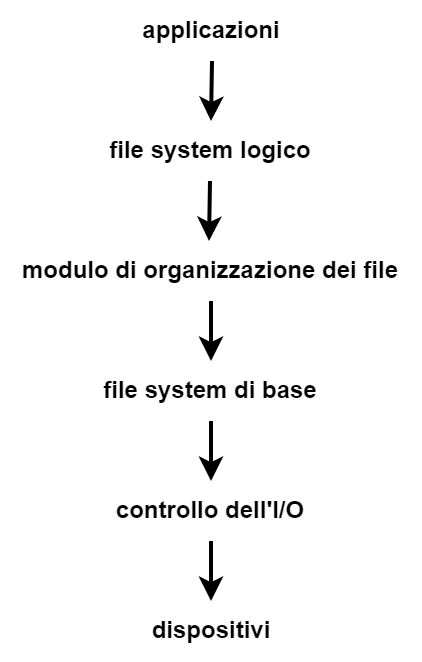
\includegraphics[width=0.35\textwidth]{img/img9.png}
        \caption{File system stratificato.}
        \label{fig:img9}
    \end{figure}
    
    \newpage
    
    Il livello più basso, il \textbf{controllo dell'I/O}, costituito semplicemente dei driver dei dispositivi e dai gestori dei segnali di interruzione, è impiegato per semplici scambi di informazioni fra memoria principale e secondaria. I driver dei dispositivi possono essere visti come traduttori che prendono in input istruzioni ad alto livello e le traducono in istruzioni adatte all'hardware, in base al controllore di I/O dedicato.
    
    Il \textbf{file system di base} deve solo inviare generici comandi all'appropriato dispositivo per leggere e scrivere blocchi fisici nel disco. Si occupa inoltre di gestire il buffer e la cache del file system. Il buffer contiene blocchi ancora da scrivere nel disco, e deve essere quindi esteso o svuotato quando si riempie, mentre la cache contiene metadati usati frequentemente dal file system, aumentandone le prestazioni. La gestione efficiente di queste due strutture risulta quindi piuttosto importante.
    
    Il modulo di \textbf{organizzazione dei file} è a conoscenza dei file e dei loro blocchi logici. Può quindi eseguire la traduzione da blocchi logici a fisici, che il livello inferiore dovrà poi trasferire, ricordando che mentre i blocchi logici sono numerati da $0$ a $1-n$, quelli fisici non rispettano una numerazione così ordinata. Questo modulo gestisce anche lo spazio libero.
    
    Infine, il \textbf{file system logico} gestisce i metadati; si tratta di tutto il contenuto del file system, eccetto gli effettivi dati contenuti nei file. Mantiene le strutture di file tramite i \textbf{blocchi di controllo dei file} (\textit{file control block}, FCB), detti \textbf{inode} nei file system UNIX, contenti informazioni sui file come la proprietà, i permessi, etc.
    
    Nei file system stratificati la duplicazione di codice è ridotta al minimo, in quanto si sfrutta molto il riuso di codice fra i vari file system. Purtroppo la stratificazione può generare un maggiore overhead del sistema operativo che può causare un decadimento delle prestazioni.
    
    Ad ogni modo la ricerca e lo sviluppo in campo di file system resta una questione aperta e ancora soggetti a customizzazioni problem-specific e miglioramenti.
    
\section{Operazioni del file system}
    Come detto in precedenza, per permettere l'accesso ai file i file system forniscono le chiamate \texttt{open()} e \texttt{close()}. Approfondiamo le strutture dati e le operazioni usate per realizzare le operazioni del file system.
    
    \subsection{Panoramica}
        Per realizzare i file system si utilizzano parecchie strutture dati, sia nei dischi sia in memoria. Sui dischi, il file system contiene informazioni su come avviare un sistema operativo memorizzato sul disco stesso, il numero totale di blocchi, il numero e la posizione dei blocchi liberi, la struttura delle directory e i singoli file.
        
        Fra le strutture presenti nei dischi troviamo tipicamente le seguenti.
        \begin{itemize}
            \item Il \textbf{blocco di controllo dell'avviamento} (\textit{boot control block}), che per ogni volume contiene informazioni utili all'avvio di un sistema operativo da quel volume; se il volume non contiene un sistema operativo, questo blocco può essere vuoto.
            
            \item Il \textbf{blocco di controllo del volume} (\textit{volume control block}); ciascuno di essi contiene i dettagli riguardanti il rispettivo volume, come il numero e la dimensione dei blocchi totali, liberi e i relativi puntatori.
            
            \item La \textbf{struttura della directory} (una per file system), usata per organizzare i file.
            
            \item Il \textbf{blocco di controllo del file} (FCB), contenente molti dettagli del relativo file.
        \end{itemize}
        
        Le informazioni tenute in memoria servono sia per la gestione del file system sia per migliorarne le prestazioni tramite l'uso di cache. I dati di caricano al momento del montaggio, si modificano durante l'utilizzo e si cancellano al momento dello smontaggio. Le strutture che vi possono essere incluse sono di vario tipo:
        \begin{itemize}
            \item La \textbf{tabella di montaggio} che contiene informazioni relative a ciascun volume montato.
            
            \item Una \textbf{cache della struttura della directory}, contenente le informazioni rilevanti relative alle directory cui i processi hanno avuto accesso recentemente.
            
            \item La \textbf{tabella di sistema dei file aperti}, contenente una copia dell'FCB per ciascun file aperto, insieme con altre informazioni.
            
            \item I \textbf{buffer} che conservano blocchi del file system durante la loro lettura o scrittura su disco.
        \end{itemize}
        
        Le applicazioni, per creare un nuovo file, eseguono una chiamata al file system logico, il quale conosce la struttura delle directory. Per creare un nuovo file, crea un nuovo FCB. Il sistema quindi carica in memoria e aggiorna la directory appropriata.
        
    \subsection{Utilizzo}
        Una volta creato un file, per essere usato per operazioni di I/O deve essere \textit{aperto}. La chiamata di sistema \texttt{open()} controlla innanzitutto se il file è già aperto, nel qual caso aggiunge un elemento alla tabella del processo che punta all'elemento corrispondente della tabella globale, metodo che fa risparmiare molto overhead da parte del sistema. In caso contrario apre il file nella tabella di sistema e punta a quest'ultimo dalla tabella del processo. Il nome dato all'elemento della tabella è detto \textit{file descriptor} in UNIX e \textit{file handle} in Windows.
        
        Quando un file viene invece chiuso la sua entry nella tabella dei file del processo viene eliminata e il contatore nella tabella di sistema viene decrementato. Ricordiamo che se questo contatore arriva a 0, la entry viene eliminata anche dalla tabella di sistema. Alcuni sistemi operativi complicano ulteriormente questo sistema, riadattando il file system per cose come connessioni di rete.
        
        Altra questione da non trascurare è quella dell'utilizzo delle \textbf{cache} quando possibile. Molti sistemi operativi hanno in cache tutti i metadati dei file aperti tranne i blocchi di dati effettivi.
        
\section{Realizzazione delle directory}
    Chiaramente la selezione di algoritmi di gestione delle directory ha un grande impatto sull'efficienza. Discutiamo ora i trade off di alcuni di questi algoritmi.
    
    \subsection{Lista lineare}
        Il concetto più semplice consiste nell'implementazione di una lista lineare che contiene i nomi dei file con puntatori ai blocchi dei dati. La sua esecuzione è tuttavia onerosa in termini di tempo. Per creare un file dobbiamo analizzare l'intera directory per verificare che non esista un file con lo stesso nome e accodare nel caso quello nuovo. Per la cancellazione dobbiamo scorrere nel caso peggiore l'intera directory per individuare il file da cancellare e fare lo shift degli elementi sulla destra.
        
        Alcuni semplici metodi di ottimizzazione comprendono il contrassegnare i file "liberi" anziché cancellarli, con un nome speciale o un bit di identificazione, oppure usare una lista concatenata per evitare lo shift degli elementi a destra dei cancellati.
        
        In generale il vero svantaggio di una lista è la ricerca dell'intera lista per trovare un file. L'utilizzo di una cache o l'impiego di una lista ordinata può ridurre l'overhead necessario, pur non risolvendo del tutto il problema.
        
    \subsection{Tabella hash}
        Abbiamo una tabella \textbf{hash} che prende in input un valore calcolato a partire dal nome dal file e restituisce un puntatore a un elemento della lista lineare contenente i puntatori dei file della directory.
        
        La ricerca, la creazione e la cancellazione di un file sono abbastanza semplici, anche se bisogna gestire i casi in cui si ottengono \textbf{collisioni}, ossia in cui due nomi di file diversi risultano nella stessa chiave.
        
        Il problema principale della tabella hash è la sua dimensione fissa e legata alla funzione hash. Se abbiamo una tabella di 64 elementi e la cui funzione può calcolare valori da 0 a 63. L'aggiunta di un 65esimo elemento implica l'estensione della tabella e il ricalcolo dei valori per una nuova funzione.
        
        Un'altra soluzione potrebbe essere l'avere gli elementi della tabella come teste di liste concatenate anziché singoli elementi. Questo è più lento perché richiede l'attraversamento di una lista in caso di collisioni, ma verosimilmente più efficiente di una semplice lista lineare.
        
\newpage
\section{Metodi di allocazione}
    La natura ad accesso diretto dei dischi li rende adatti ad accogliere file. Tuttavia ci sono diversi modi di allocare la memoria per i file in maniera più o meno efficiente. Esistono tre modi principali di farlo, che andremo qui a vedere. Chiaramente ognuno di essi presenta vantaggi e svantaggi. Alcuni sistemi dispongono di tutti e tre i modi, ma è più comune vederne uno solo su un singolo sistema.
    
    \subsection{Allocazione contigua}
        Questo metodo prevede l'occupazione di un insieme di blocchi \textbf{contigui} nel disco. In questo caso il numero di riposizionamenti della testina (\textit{seek}) per accedere a un singolo file è minimo. L'elemento di directory che descrive un file ne indica la posizione del primo blocco e la lunghezza, dai quali si può chiaramente ricavare la locazione dell'intero file.
        
        Questo metodo gestisce in modo semplice sia l'accesso sequenziale (basta accedere al primo blocco e ai $n$ successivi per lunghezza di $n$) che quello diretto (se vogliamo accedere al blocco $i$, e considerando il primo blocco indicato dalla entry della directory come $b$, ci basta accedere al blocco $b+i$).
        
        Un primo problema che troviamo con questa allocazione è l'individuazione dello spazio libero per un nuovo file, che non è immediata. Possiamo immaginare questo problema come una versione meno generale del problema dell'\textit{allocazione dinamica della memoria}, in cui dobbiamo soddisfare una richiesta di una certa dimensione data una lista di buchi liberi. Ricordiamo che i criteri più comuni di scelta di un buco libero sono \textit{best-fit} e \textit{first-fit}. Questi algoritmi soffrono della \textbf{frammentazione esterna}: lo spazio libero viene frammentato infatti in tanti piccoli buchi, che riuscirebbero ad accomodare un file (o molti file) se fossero contigui, ma non lo sono.
        
        Un metodo di \textbf{compattazione} sta nel trasferire tutti i file in un secondo file system e ricopiarli poi nello spazio libero lasciato nel primo in maniera contigua. Questo metodo funge effettivamente da deframmentazione, e spesso viene eseguito \textbf{off-line}, ossia con il file system non montato e quindi rende il sistema inutilizzabile. Oggi vari metodi di deframmentazione lasciano il sistema in uno stato utilizzabile ma a basse prestazioni.
        
        Un altro problema non da poco è l'allocazione dello spazio giusto per un file. Soprattutto per quanto riguarda file soggetti a una certa estensione, che devono per esempio contenere dati prodotti da un file, l'assegnazione di troppo spazio crea frammentazione, l'assegnazione di troppo poco spazio non gli permette di estendersi. La prima e poco desiderabile soluzione è terminare il programma utente con un appropriato messaggio di errore, il quale dovrà allocare più spazio e rieseguire il programma. L'altra soluzione consiste nel trovare un buco più grande, copiarvi il contenuto e rilasciare lo spazio previamente occupato.
        
        Anche conoscendo previamente lo spazio che un file andrà a occupare, il problema non viene risolto: se questo file cresce lentamente, durante la sua crescita ci sarà frammentazione interna.
        
        Alcuni sistemi operativi inizializzano un certo spazio in un primo momento e secondo necessità inseriscono poi una continuazione di questo spazio contiguo detta \textbf{estensione}. Il file si registrerà come il primo blocco, il numero di blocchi \textbf{e} la locazione del primo blocco della prossima estensione. Anche questa soluzione non è perfetta, in quanto le estensioni possono essere soggette a frammentazione esterna come i file originali.
        
    \subsection{Allocazione concatenata}
        Questo metodo risolve tutti i problemi dell'allocazione contigua. Il file è memorizzato come una lista concatenata che può essere sparsa in qualsiasi ordine sul disco. La directory contiene un puntatore al primo e all'ultimo blocco del file. Ogni blocco contiene chiaramente un puntatore al blocco successivo.
        
        Per creare un file, si crea semplicemente la entry nella directory che punta al primo blocco. Estendere il file consta semplicemente dell'atto di cercare il prossimo blocco vuoto tramite il sistema di gestione dello spazio libero e concatenarlo alla lista. La lettura è ancora più semplice, in quanto basta leggere i blocchi in sequenza. Questo metodo non implica nessun tipo di frammentazione esterna, e inoltre non richiede la computazione di nessuno spazio libero, in quanto il file può semplicemente continuare a crescere finché non vengono terminati i blocchi liberi.
        
        L'allocazione concatenata presenta comunque alcuni svantaggi. Quello principale sta nel fatto che può essere usata efficientemente solo nei file ad accesso sequenziale. Per trovare un arbitrario $i$-esimo blocco, occorre iniziare dal primo e percorrere $i$ blocchi. Su un HDD questo è oneroso in quanto la lettura del blocco successivo implica una lettura in memoria e talvolta il riposizionamento della testina.
        
        Un altro svantaggio sta nello spazio richiesto. Il puntatore al blocco successivo va memorizzato nel blocco, e se prendiamo per esempio puntatori dei 4 byte, lo 0,74\% del file è usato per memorizzare puntatori.
        
        La soluzione più comune a ciò consiste nel riunire più gruppi contigui di blocchi in \textbf{cluster}, e nell'allocare i cluster anziché i blocchi singoli. Essendo questa una via di mezzo fra i due metodi visti fino ad ora ne eredita parte dei vantaggi e degli svantaggi: mantiene la semplice corrispondenza fra memoria fisica e logica, aumenta il throughput rispetto all'allocazione concatenata in quanto richiede meno letture e riposizionamenti della testina, meno memoria è occupata per i puntatori, ma abbiamo allo stesso tempo più frammentazione interna. I cluster sono comunque molto impiegati nella realizzazione di file system in quanto possono ottimizzare l'accesso ai dischi in molti altri algoritmi.
        
        Un altro problema dell'allocazione concatenata è l'affidabilità. Siccome i file sono lunghe catene di blocchi tenuti insieme da puntatori sparsi per tutto il disco, si immagini cosa possa accadere qualora un puntatore andasse perduto o danneggiato. La lettura di un puntatore in maniera errata potrebbe causare la il collegamento alla lista dei blocchi liberi o di un altro file. Possibili soluzioni possono essere usare una lista doppiamente concatenata o la memorizzazione del nome del file e del relativo numero di blocco in ogni blocco; chiaramente questo aumenta considerevolmente sia spazio occupato da ogni file che overhead.
        
        Una variante importante del metodo di allocazione concatenata consiste nell'impiego della \textbf{tabella di allocazione dei file} (\textit{file allocation table}, FAT). Per contenere tale tabella si riserva parte dello spazio del disco all'interno di ogni volume; la FAT ha un elemento per ogni blocco del disco ed è indicizzata dal numero di blocco; si usa essenzialmente come una lista concatenata. L'elemento della directory contiene il numero del primo blocco del file. L'elemento della tabella così indicizzato contiene quindi il successivo e così via fino all'ultimo blocco che contiene un valore speciale di fine del file. I blocchi inutilizzati sono indicati nella tabella con il valore 0. L'allocazione di un nuovo blocco richiede semplicemente l'individuazione del primo blocco vuoto della tabella e la sostituzione di quel valore con l'inizio del blocco precedente.
        
    \subsection{Allocazione indicizzata}
        L'allocazione concatenata risolve i problemi della dichiarazione delle dimensioni del file e della frammentazione esterna presenti nel metodo di allocazione contigua. Tuttavia, senza la presenza di una FAT, l'allocazione concatenata soffre per quanto riguarda l'accesso diretto. L'\textbf{allocazione indicizzata} risolve questo problema raggruppando tutti i puntatori in un solo blocco: il \textbf{blocco indice}.
        
        Ogni file ha il proprio blocco indice: si tratta di un array di indirizzi di blocchi del disco: L'$i$-esimo elemento del blocco indice punta all'$i$-esimo blocco del file. La entry della directory contiene l'indirizzo del blocco indice. L'allocazione di nuovi blocchi consta semplicemente nel cercare il prossimo blocco impostato a \texttt{null} e riempirlo. La frammentazione esterna non sussiste e l'accesso diretto è intuitivo.
        
        Chiaramente per file molto piccoli, andiamo ad allocare un intero blocco indice, anche se quasi tutti i puntatori sono impostati a \texttt{null}, il che è uno spreco di memoria.
        
        Questo punto solleva la questione della dimensione del blocco indice. Un blocco troppo grande causa uno spreco di spazio (potrebbe essere quasi visto come frammentazione interna), mentre uno troppo piccolo potrebbe non riuscire a indicizzare tutti i blocchi del file. Fra i possibili meccanismi ci sono i seguenti:
        \begin{itemize}
            \item \textbf{Schema concatenato.} Possiamo immaginare più blocchi indice concatenati fra loro. Abbiamo un primo blocco piccolo che contiene il nome del file e i primi indirizzi, che può terminare con \texttt{null} o un puntatore all'inizio del prossimo blocco.
            
            \item \textbf{Indice a più livelli.} Questo meccanismo prevede la presenza di un primo indice che punta ad altri indici, i quali puntano ai blocchi del file. In base a necessità il numero di livelli potrebbe anche aumentare.
            
            \item \textbf{Schema combinato.} Un'altra possibilità, realizzata per esempio nei sistemi basati su UNIX, è quella di posizionare i primi blocchi effettivi nell'\textit{inode} del file. Se il file è molto piccolo, questo basta a memorizzare l'intero file. Altrimenti, l'ultimo blocco punterà a un blocco indice. Se quello basta bene, altrimenti il \textit{suo} ultimo blocco punterà a un blocco indice a due livelli, e così via. Andiamo quindi a diminuire la granularità della soluzione quando e solo se il file è di grandi dimensioni, avendo una soluzione adattiva.
        \end{itemize}
        
        Gli schemi di allocazione indicizzata soffrono di alcuni problemi di prestazioni che abbiamo visto nell'allocazione concatenata. In particolare, gli indirizzi sono tutti nello stesso blocco, ma i blocchi puntati potrebbero essere sparsi nel volume.

\chapter{Argomenti Avanzati, Capitolo 18: Macchine Virtuali}
\section{Introduzione}
    Il concetto alla base delle macchine virtuali è di estrarre i componenti di un singolo computer in diversi ambienti di esecuzione diversi, dando così l'illusione che ogni ambiente sia in esecuzione su un computer diverso. Questo concetto è per certi affine a quello della strutturazione stratificata di un sistema operativo. Nel caso della virtualizzazione vi è uno strato che crea un ambiente in cui è possibile eseguire sistemi operativi o applicazioni.
    
    Alla base dell'intera gerarchia c'è l'\textbf{host}, che è l'hardware che gestisce le macchine virtuali, mentre il \textbf{gestore delle macchine virtuali}, o \textit{hypervisor} crea e gestisce le macchine virtuali fornendo un'interfaccia identica a quella dell'host. Ci sono poi i processi \textbf{guest}. A ognuno di questi viene fornita un copia dell'host. Di solito il processo guest è esso stesso un sistema operativo. Possono quindi esserci più sistemi operativi in esecuzione su un singolo hardware contemporaneamente, ognuno nella sua macchina virtuale.
    
    Vale la pena di notare come ciò renda la definizione di sistema operativo ancora più sfumata di quanto già non lo fosse.
    
\section{Storia}
    Le macchine virtuali hanno fatto la loro comparsa sul mercato nel 1972. La virtualizzazione era fornita dal sistema operativo IBM VM, e ha stabilito dei concetti rilevanti ancora oggi.
    
    Una delle principali difficoltà riguardava i dischi. Era difficile eseguire più sistemi operativi di quanti fossero i dischi, e la soluzione arrivò sotto forma dei \textbf{minidisk}. Essi erano identici sotto ogni aspetto ai dischi fisici tranne che per dimensione, e il sistema li implementava allocando le tacce sui dischi fisici di cui il minidisk aveva bisogno.
    
    La virtualizzazione si è diffusa anche grazie a una sua definizione formale, che richiedeva i seguenti requisiti:
    \begin{itemize}
        \item \textbf{Fedeltà.} Un VMM deve fornire un ambiente per i programmi essenzialmente identico alla macchina originale.
        \item \textbf{Prestazioni.} La perdita di prestazioni per i programmi in esecuzione nell'ambiente virtuale deve essere modesta.
        \item \textbf{Sicurezza.} Il VMM è in completo controllo delle risorse del sistema.
    \end{itemize}
    
\section{Vantaggi e caratteristiche}
    I vantaggi della virtualizzazione e delle macchine virtuali sono molteplici. Innanzitutto potrebbe essere appetibile avere sistemi molto omogenei sullo stesso hardware, o addirittura sulla stessa macchina.
    
    Un'altra caratteristica molto importante riguarda la sicurezza: essendo i sistemi separati dall'host e separati fra loro, fungono essenzialmente da \textit{sandbox}. Se un virus dovesse infettare un sistema operativo, potrebbe causare danni al sistema stesso, ma difficilmente questi danni si estenderanno al sistema host o alle altre macchine virtuali.
    
    L'altra faccia della medaglia è che questo grado di isolamento può impedire la condivisione delle risorse. Una possibile soluzione è definire un volume del file system che permette la condivisione dei file. In alternativa è possibile creare una rete di macchine virtuali che possono comunicare tramite la rete fra di loro.
    
    Una caratteristica di molte macchine fisiche è la possibilità di ibernare, o \textit{sospendere} la macchina stessa, per riprenderne l'esecuzione in seguito. Le macchine virtuali portano questo concetto ancora più avanti e permettono di eseguire una copia dello stato della macchina, il quale può essere eseguito su qualsiasi altra macchina virtuale compatibile, permettendo l'effettiva creazione di \textbf{cloni}. Questa funzione può anche essere usata per creare backup e ripristinare stati precedenti della macchina, nel caso di un malfunzionamento fatale per esempio.
    
    L'utilizzo di macchine virtuali può anche aiutare gli sviluppatori di sistemi operativi. Di solito, la modifica di un sistema operativo è un'operazione delicata e pericolosa, e mentre avviene la modifica il sistema deve essere arrestato e restare inutilizzato. Utilizzare una macchina virtuale per apportare modifiche e testare il sistema operativo permette di spegnere la macchina solo quando le modifiche vanno applicate. Questo può essere utile nel caso di una macchina che fornisce servizi che hanno bisogno di un uptime costante.
    
    Un altro vantaggio di cui possono avvalersi gli sviluppatori è testare diverse versioni del proprio software su sistemi diversi senza necessariamente possedere hardware distinti. Questo vantaggio si estende anche al controllo qualità.
    
    Va considerato inoltre che gli strumenti di gestione di un VMM permettono a un amministratore di gestire molti più sistemi di quanto potrebbe fare senza il supporto di un VMM. In particolare, per esempio, il \textbf{templating} permette di avere un'immagine standard di un sistema operativo ed eseguirla su molte macchine virtuali. Ciò facilita anche backup, ripristino e controllo delle risorse.
    
    Un'altra funzione molto utile è la migrazione in tempo reale, o \textbf{live migration}, che permette di spostare l'esecuzione di un sistema operativo da un server fisico a un altro senza interruzione di servizio. Questo può essere molto utile se vogliamo liberare risorse sulla macchina iniziale, o se c'è bisogno di manutenere una macchina, in quanto possiamo spostare i suoi servizi su una seconda senza interromperli durante la manutenzione.
    
    Anche la distribuzione di applicazioni potrebbe giovare dalla diffusione di macchine virtuali, e in particolare dalla diffusione di uno standard. Potremmo infatti pensare di distribuire un sistema operativo con l'applicazione già preinstallata, e ciò, dato un formato standard per l'immagine, la renderebbe compatibile con qualsiasi macchina capace di supportare un VMM, e renderebbe anche l'aggiornamento e la manutenzione più standardizzati.
    
    Un'altra tecnologia resa disponibile in gran parte grazie alla virtualizzazione è il \textbf{cloud computing}, in quanto è possibile rendere disponibili risorse come memoria o CPU tramite Internet.

\end{document}
